\documentclass[a4paper]{article}

% Packages
\usepackage{graphicx}
\usepackage{subcaption}
\usepackage[margin=1.5cm, includefoot, footskip=30pt]{geometry}



% Title
\title{Evolution Reinforces Cooperation with the Emergence of Self-Recognition
       Mechanisms: an Empirical Study of the Moran process for the Iterated
       Prisoner's Dilemma - Online Materials}
\author{Vincent Knight}
\author{Marc Harper}
\author{Nikoleta E. Glynatsi}
\author{Owen Campbell}

\date{}

\begin{document}

\maketitle

This document contains graphical materials accompanying the manuscript entitled:
\textbf{``Evolution Reinforces Cooperation with the Emergence of Self-Recognition
Mechanisms: an Empirical Study of the Moran process for the Iterated
Prisoner's Dilemma''}.

\begin{itemize}
    \item Figures~\ref{invasion-3}-\ref{invasion-14} show the fixation probability \(x_1\)
for each strategy. The mean and error bars are shown against the collection of
all opponents.

    \item Figures~\ref{resistance-3}-\ref{resistance-14} show the fixation probability
\(x_{N-1}\) for each strategy. Again, the mean and error bars are shown against
the collection of all opponents.

    \item Figures~\ref{fig:ranks_v_size_invade}-\ref{fig:ranks_v_size_coexist} show the
ranks of each strategy according to mean absorption probability across all
population sizes.
\end{itemize}

\begin{figure}[!hbtp]
    \centering
    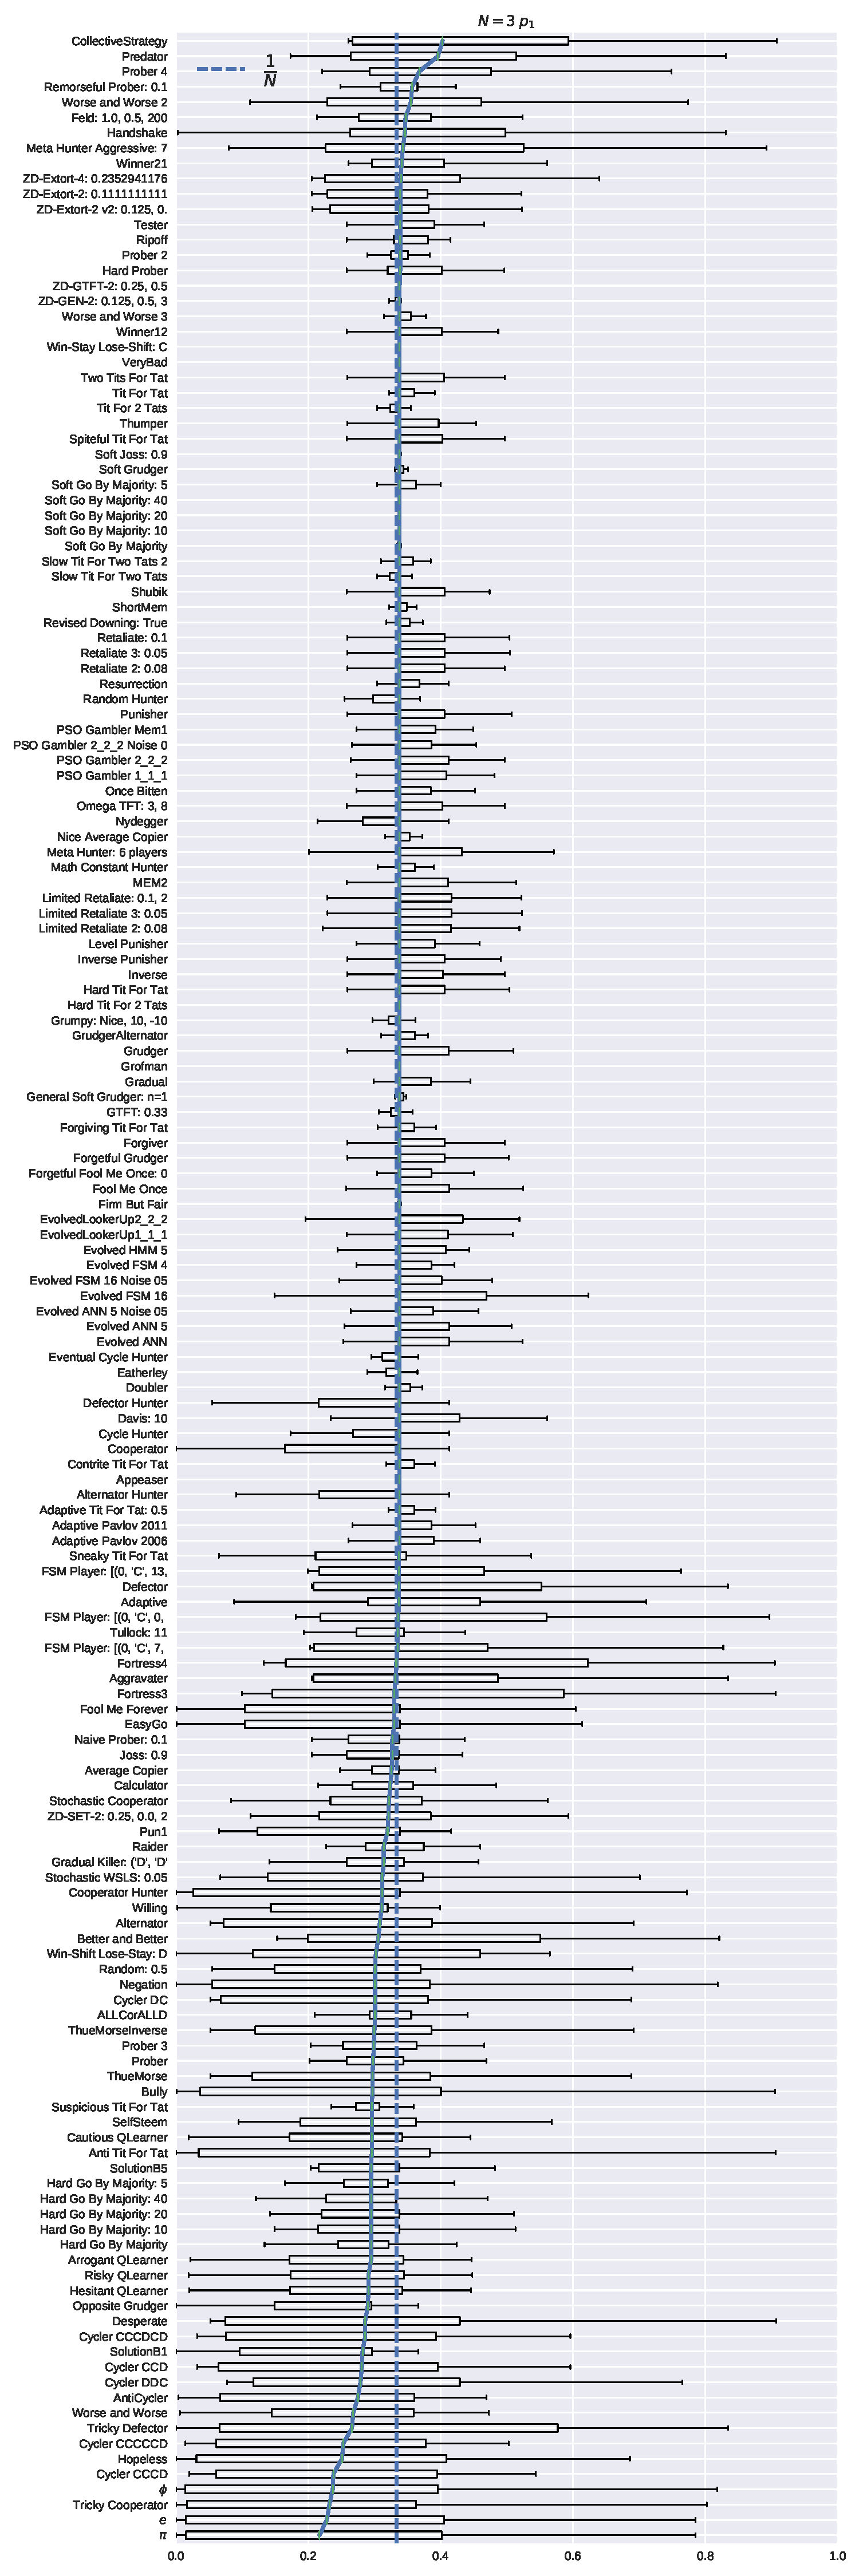
\includegraphics[width=\textwidth]{img/boxplot_3_invade.pdf}
    \caption{The fixation probabilities \(x_1\) for \(N=3\)}
    \label{invasion-3}
\end{figure}

\begin{figure}[!hbtp]
    \centering
    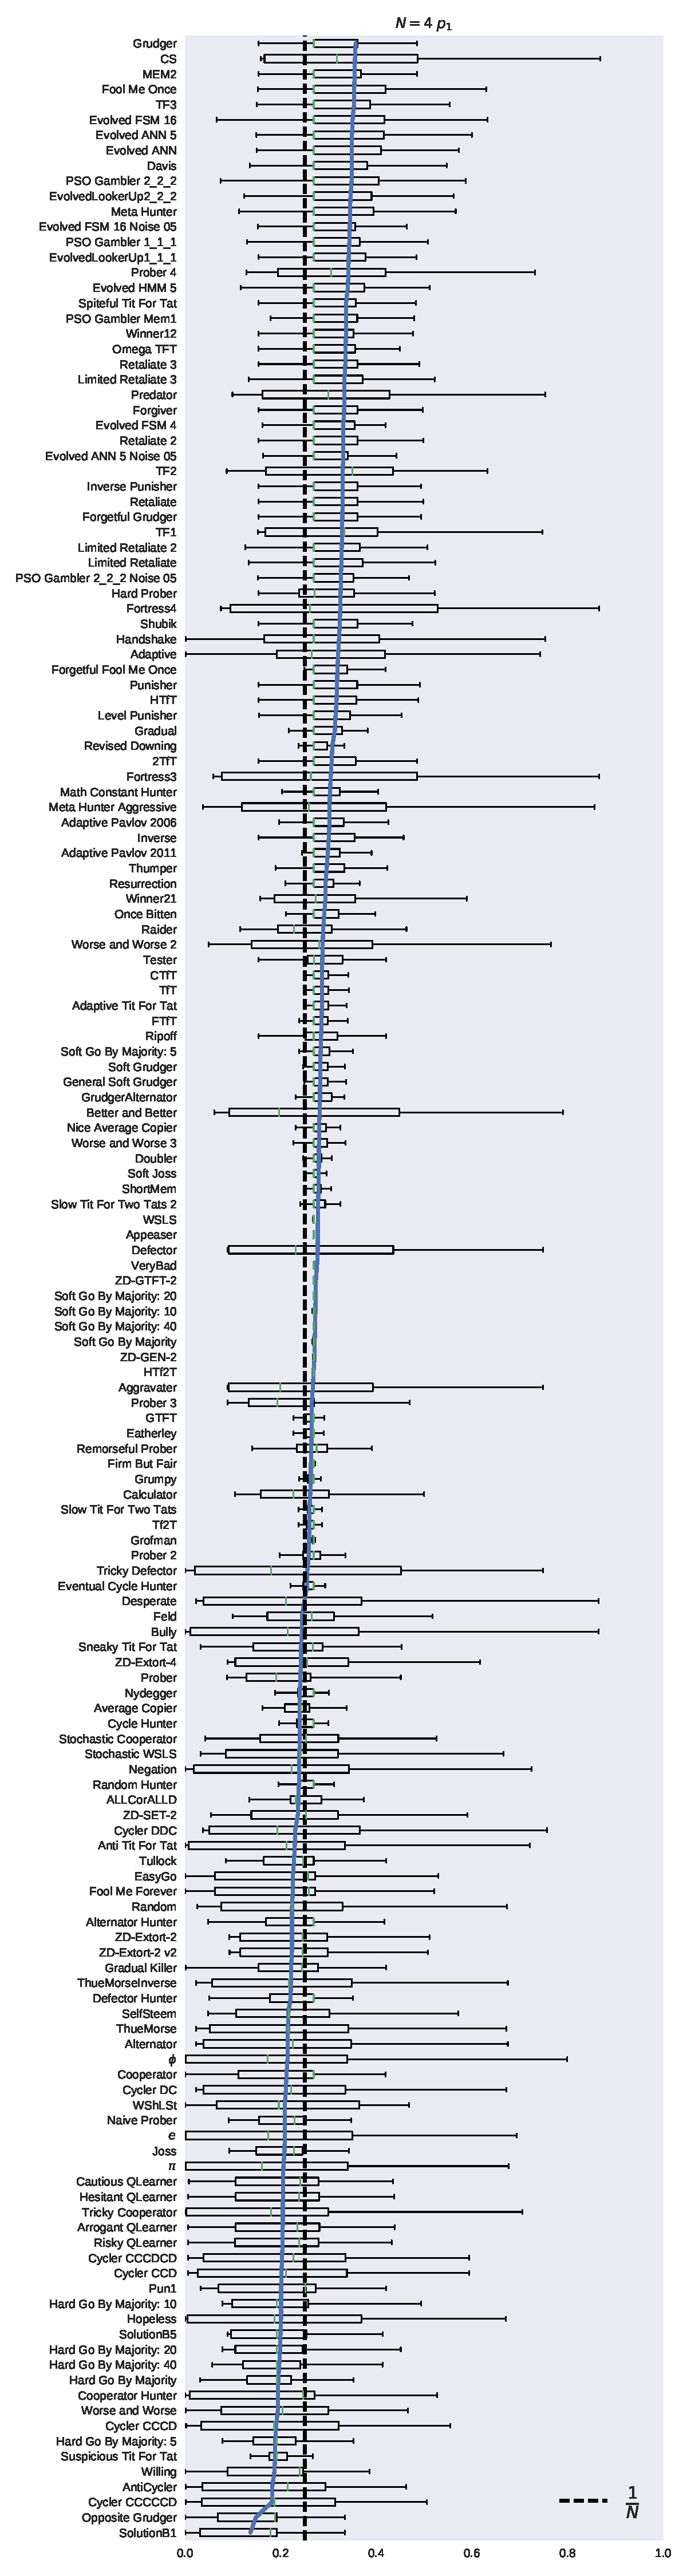
\includegraphics[width=\textwidth]{img/boxplot_4_invade.pdf}
    \caption{The fixation probabilities \(x_1\) for \(N=4\)}
\end{figure}

\begin{figure}[!hbtp]
    \centering
    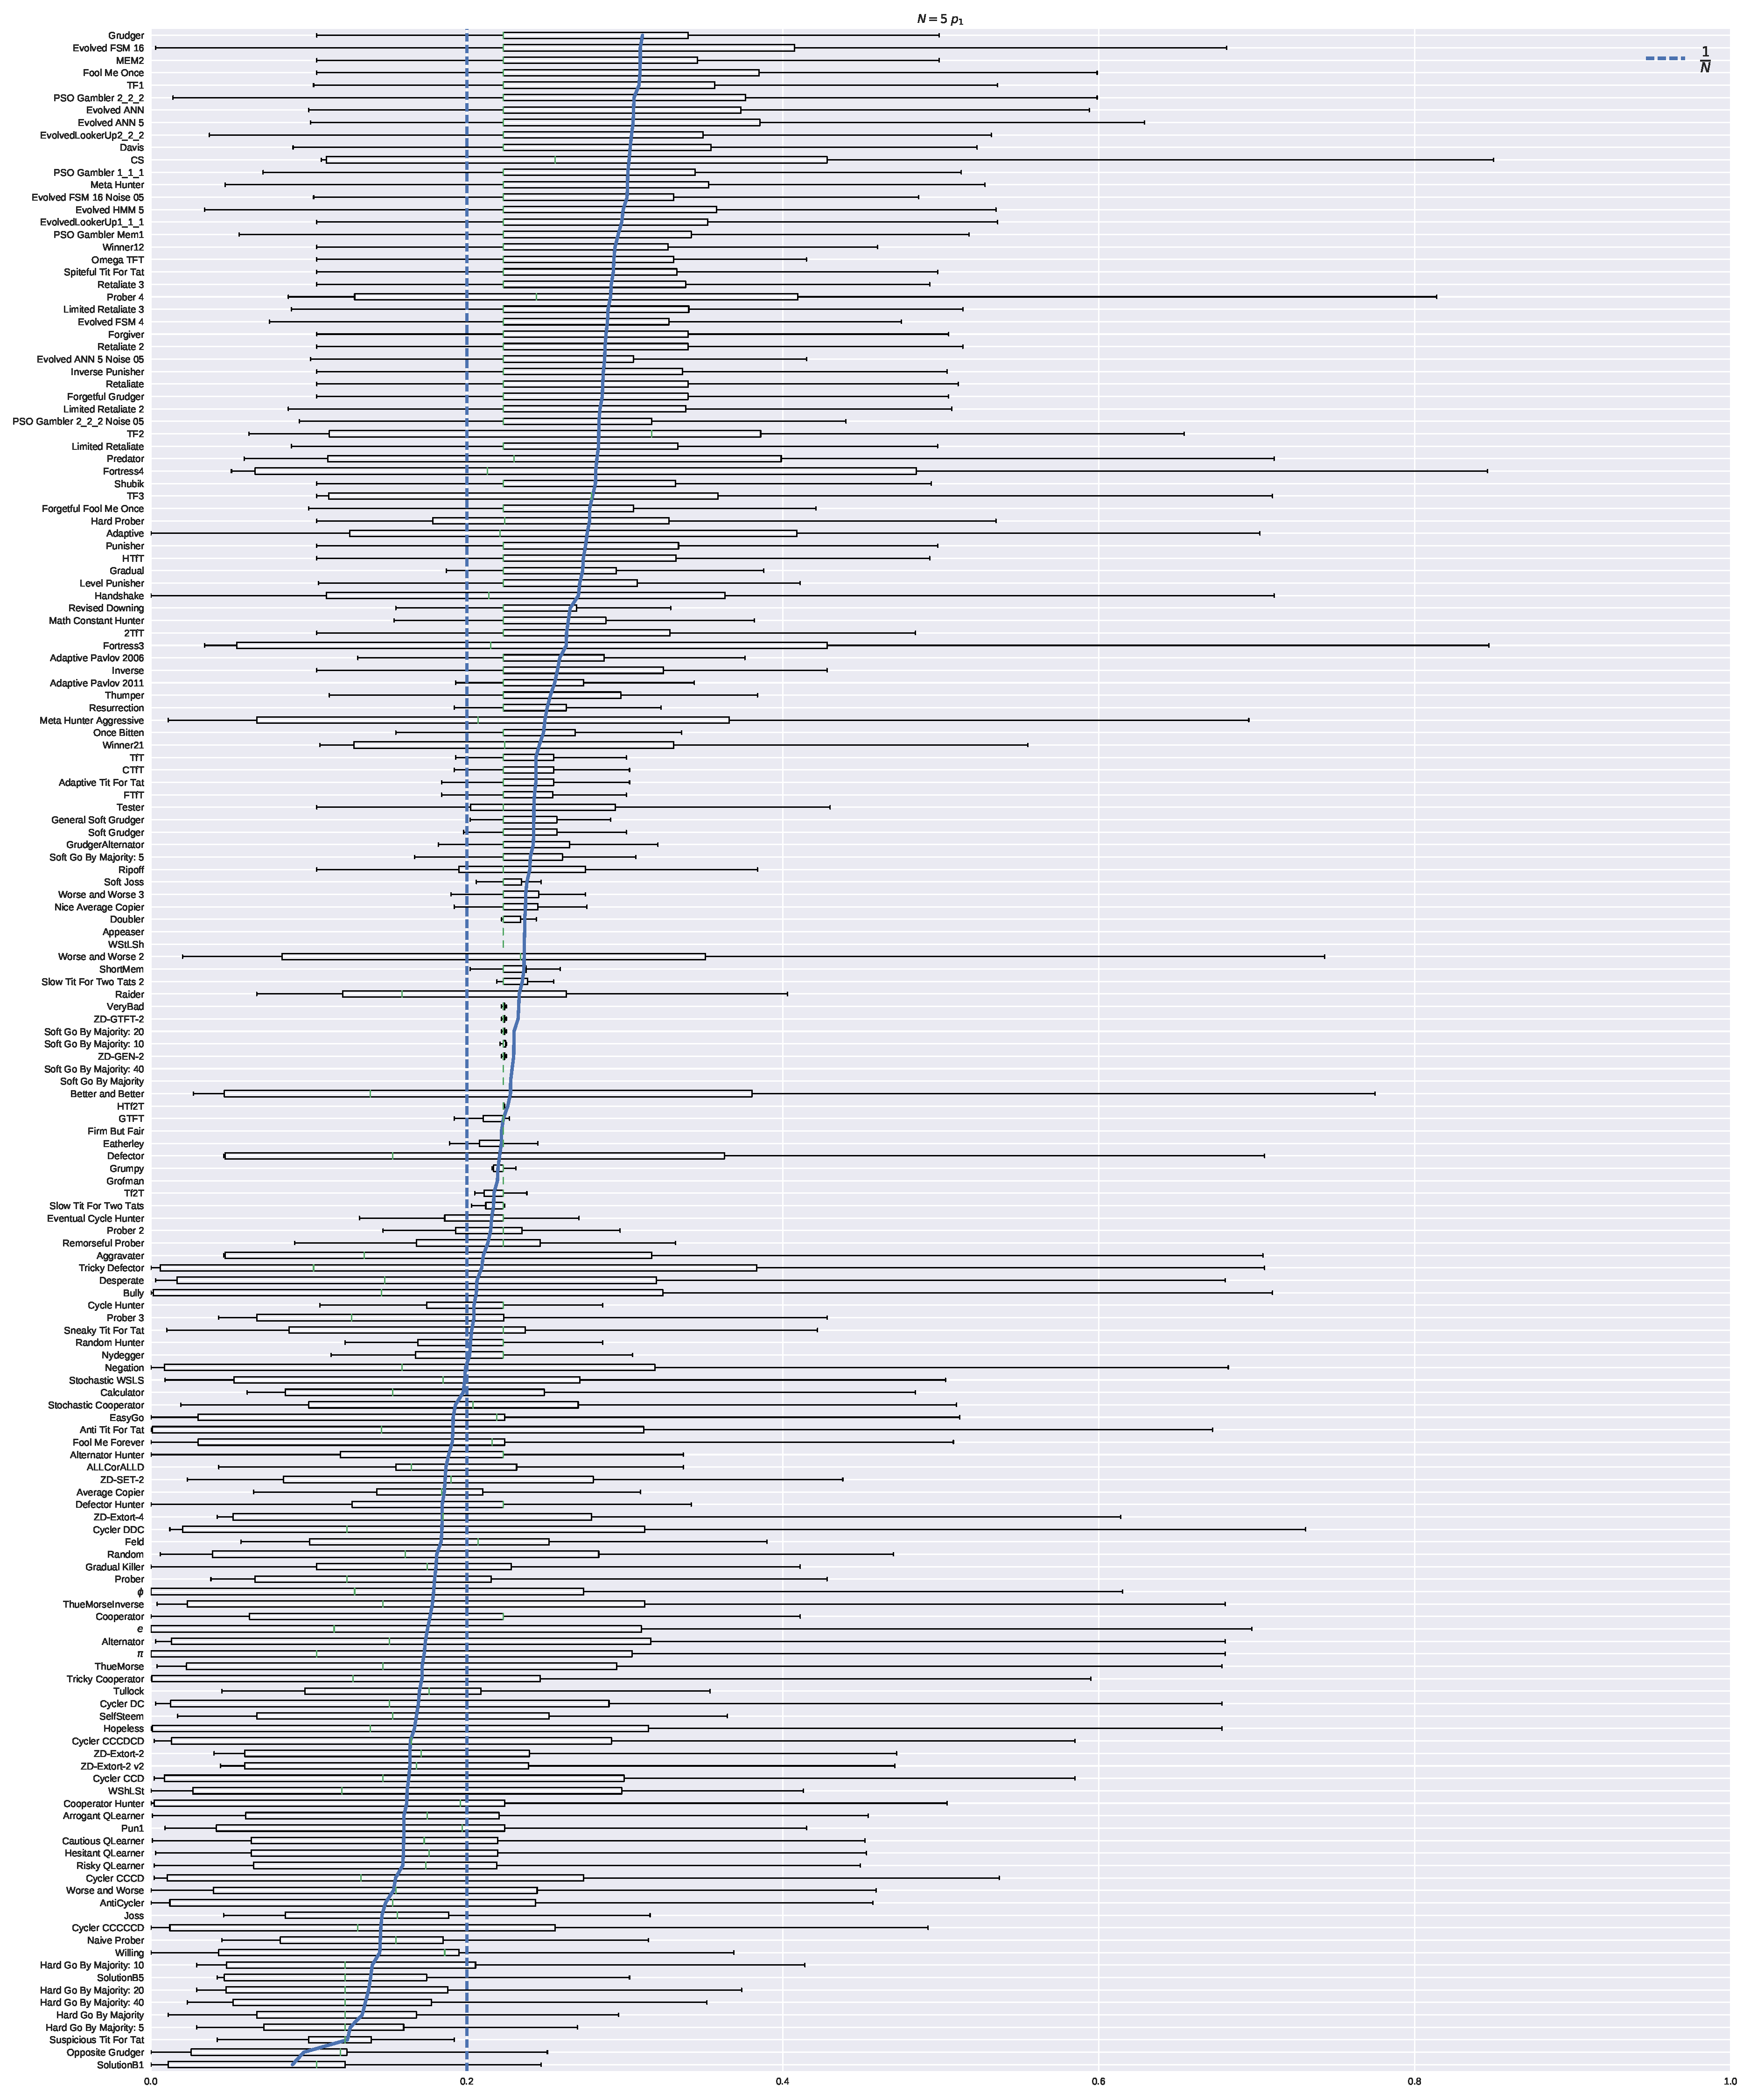
\includegraphics[width=\textwidth]{img/boxplot_5_invade.pdf}
    \caption{The fixation probabilities \(x_1\) for \(N=5\)}
\end{figure}

\begin{figure}[!hbtp]
    \centering
    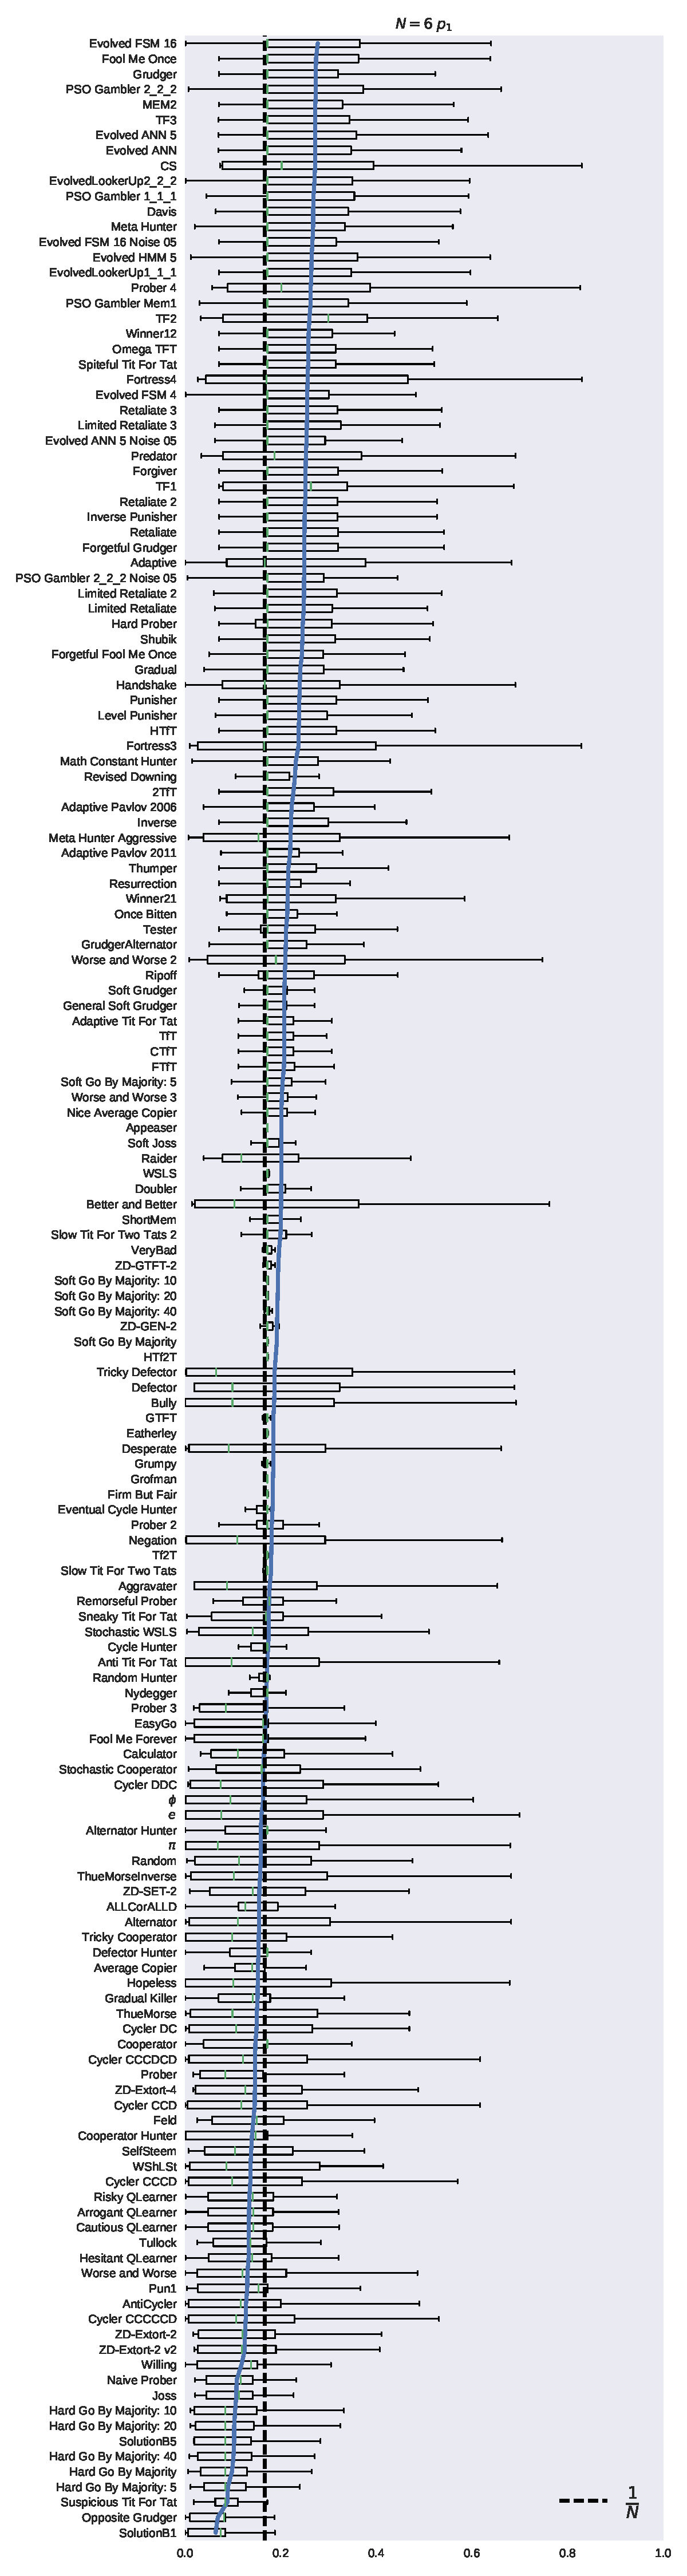
\includegraphics[width=\textwidth]{img/boxplot_6_invade.pdf}
    \caption{The fixation probabilities \(x_1\) for \(N=6\)}
\end{figure}

\begin{figure}[!hbtp]
    \centering
    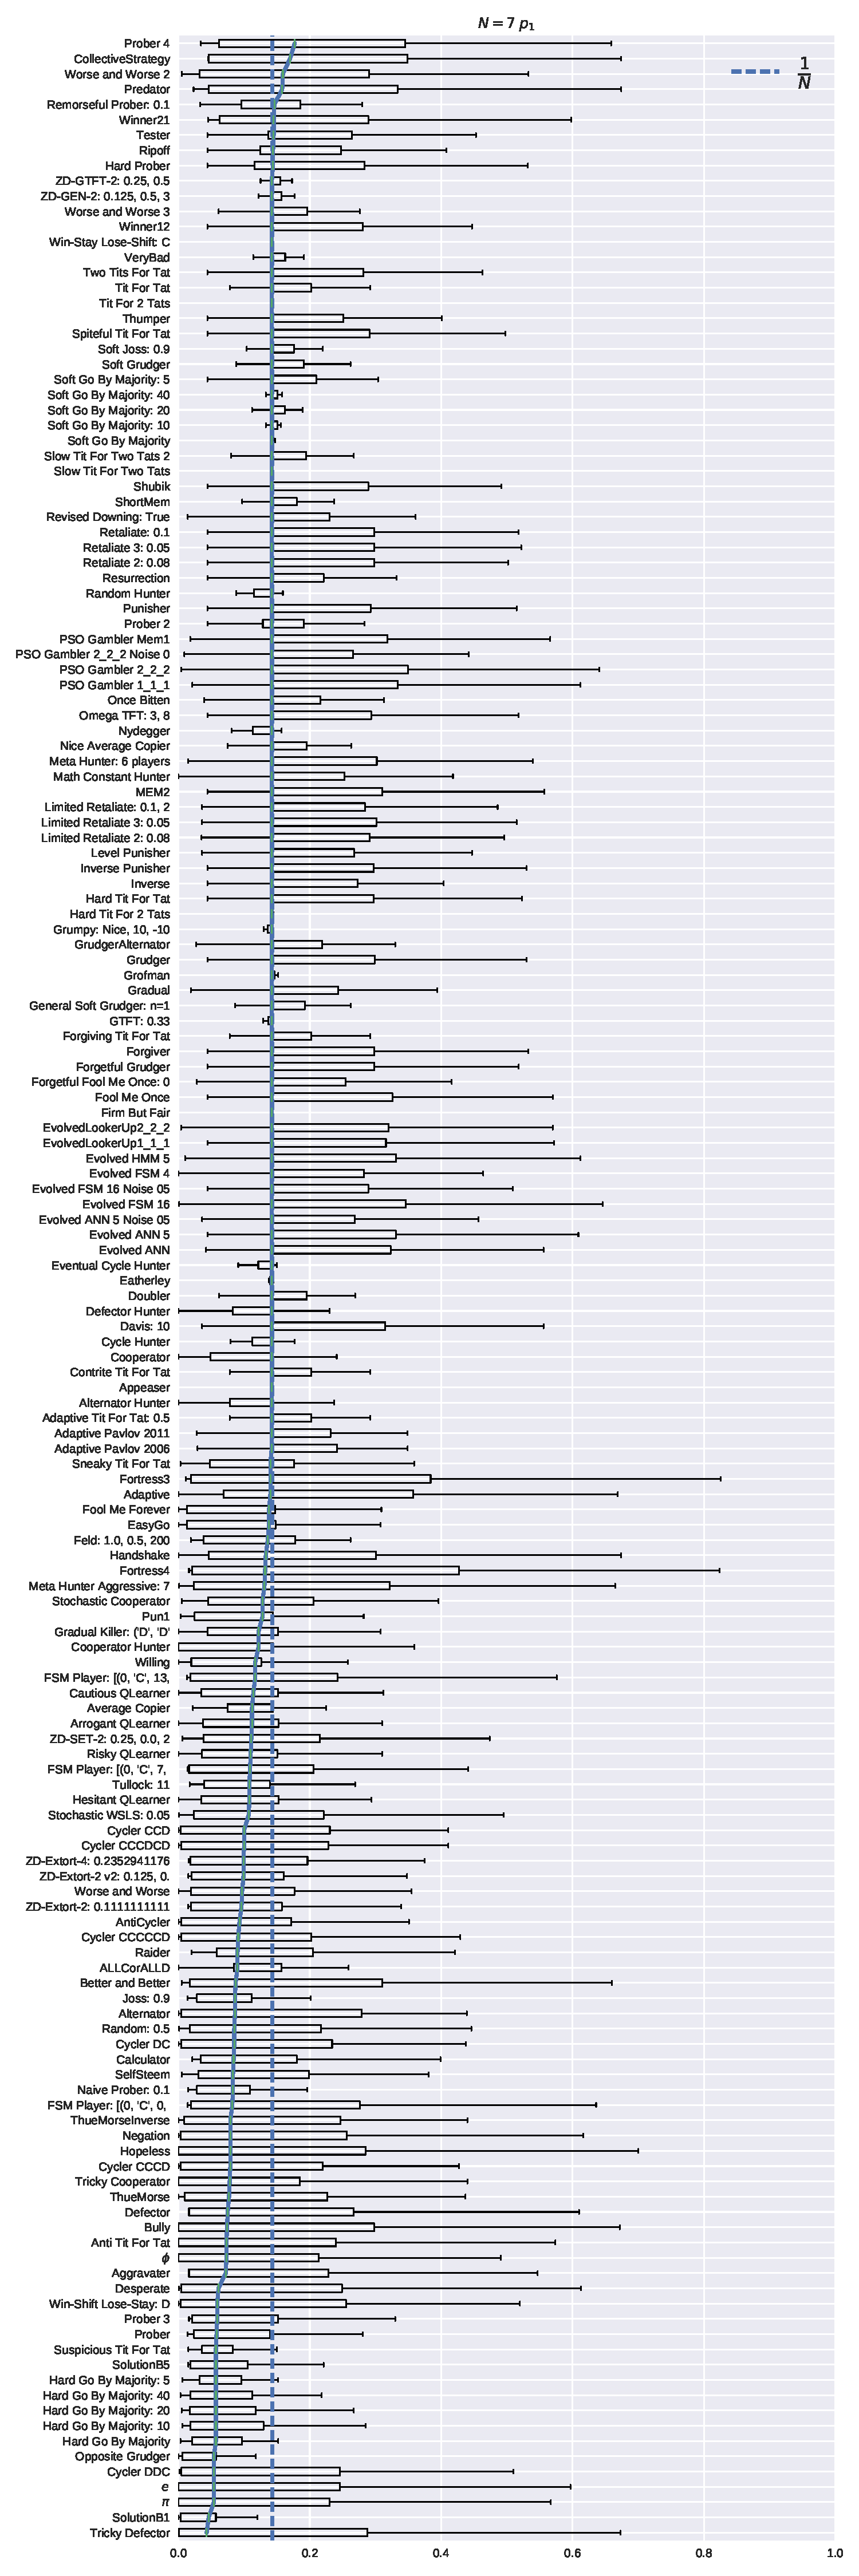
\includegraphics[width=\textwidth]{img/boxplot_7_invade.pdf}
    \caption{The fixation probabilities \(x_1\) for \(N=7\)}
\end{figure}

\begin{figure}[!hbtp]
    \centering
    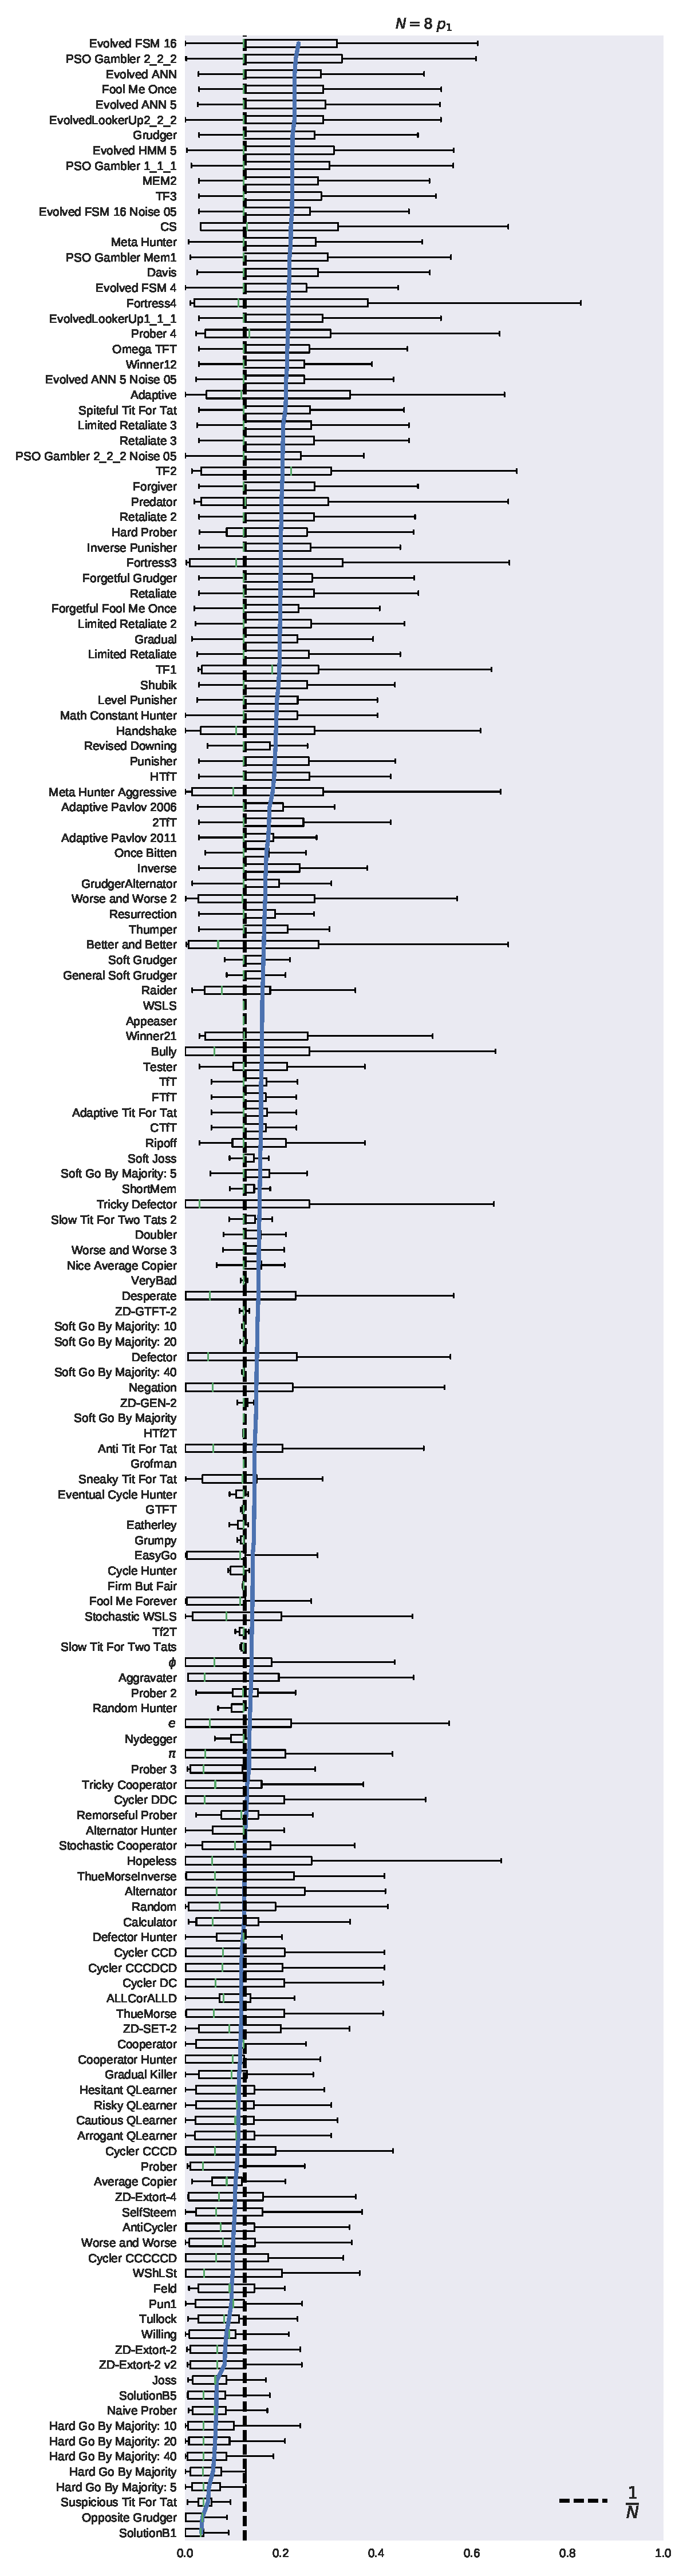
\includegraphics[width=\textwidth]{img/boxplot_8_invade.pdf}
    \caption{The fixation probabilities \(x_1\) for \(N=8\)}
\end{figure}

\begin{figure}[!hbtp]
    \centering
    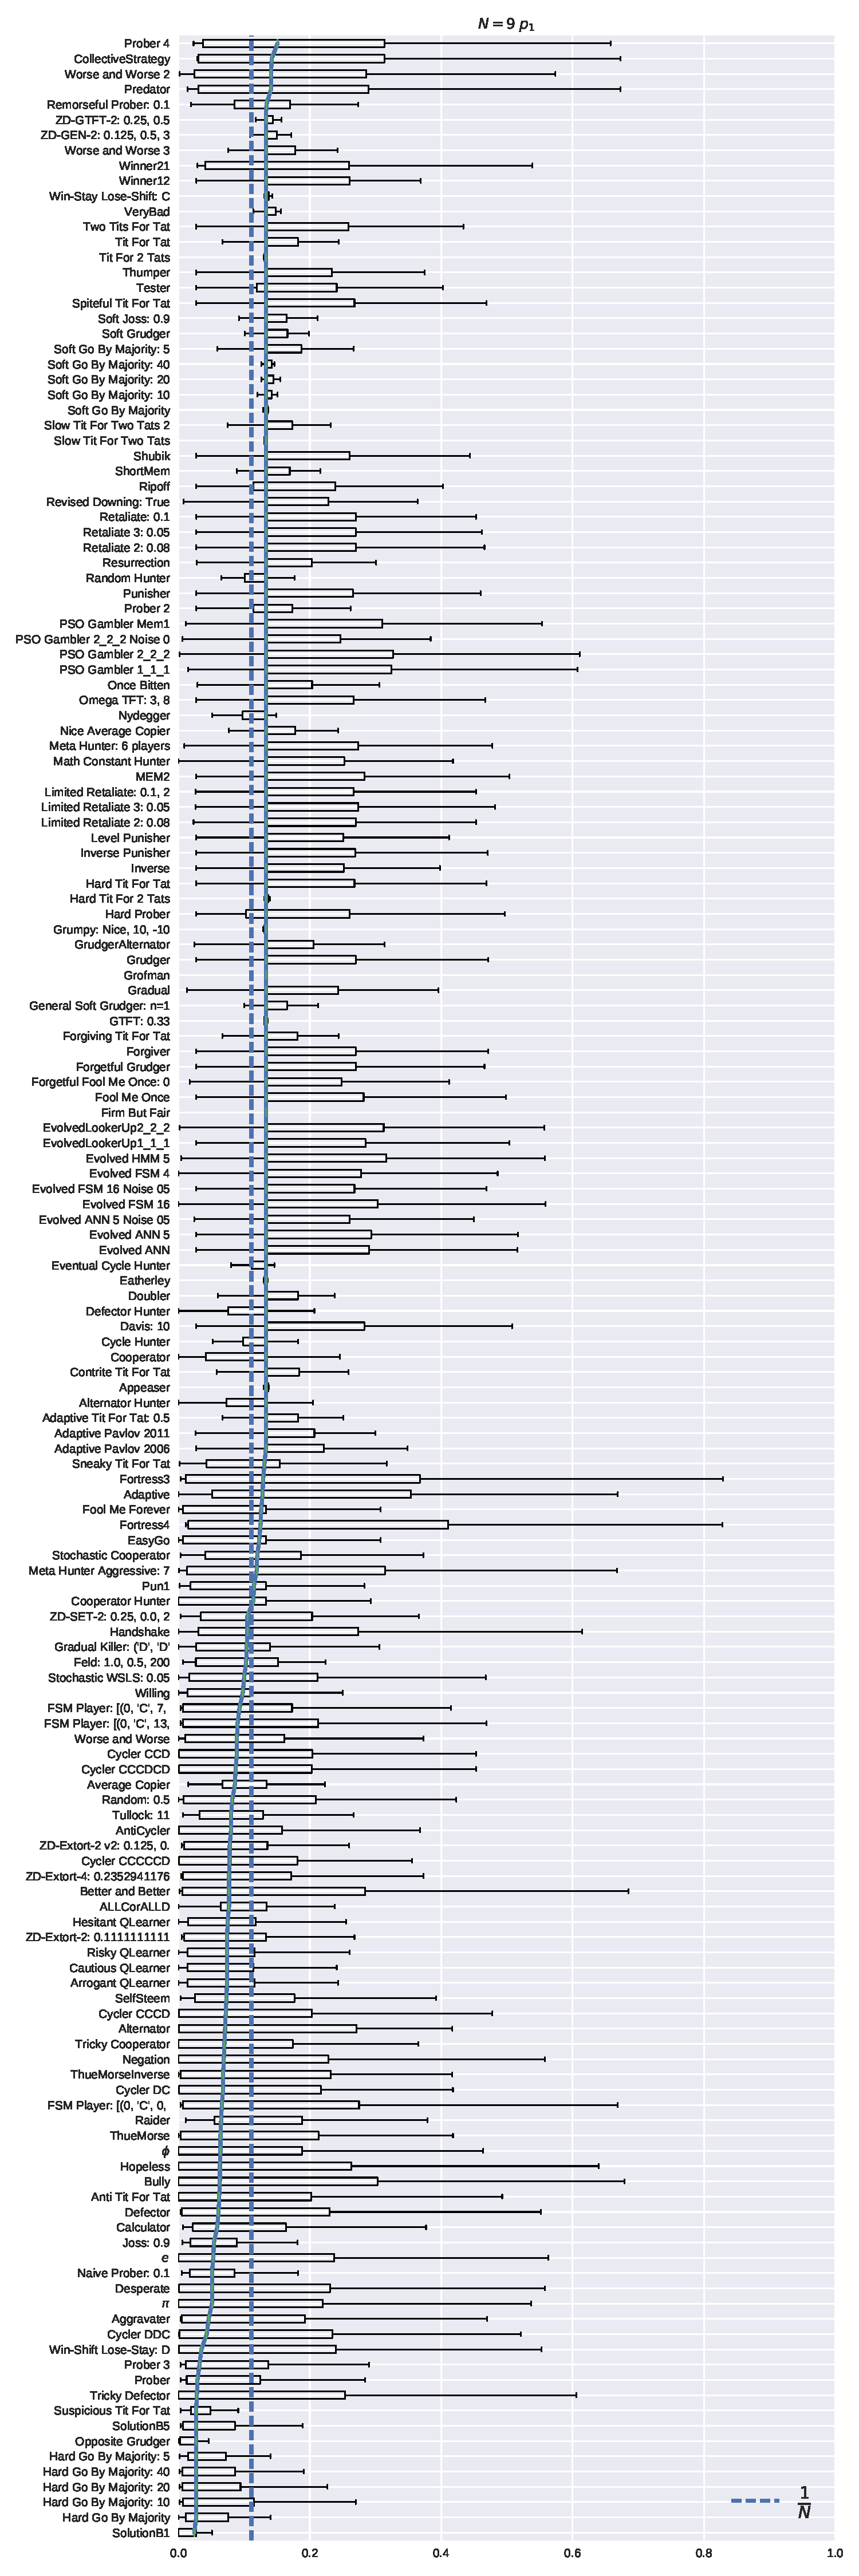
\includegraphics[width=\textwidth]{img/boxplot_9_invade.pdf}
    \caption{The fixation probabilities \(x_1\) for \(N=9\)}
\end{figure}

\begin{figure}[!hbtp]
    \centering
    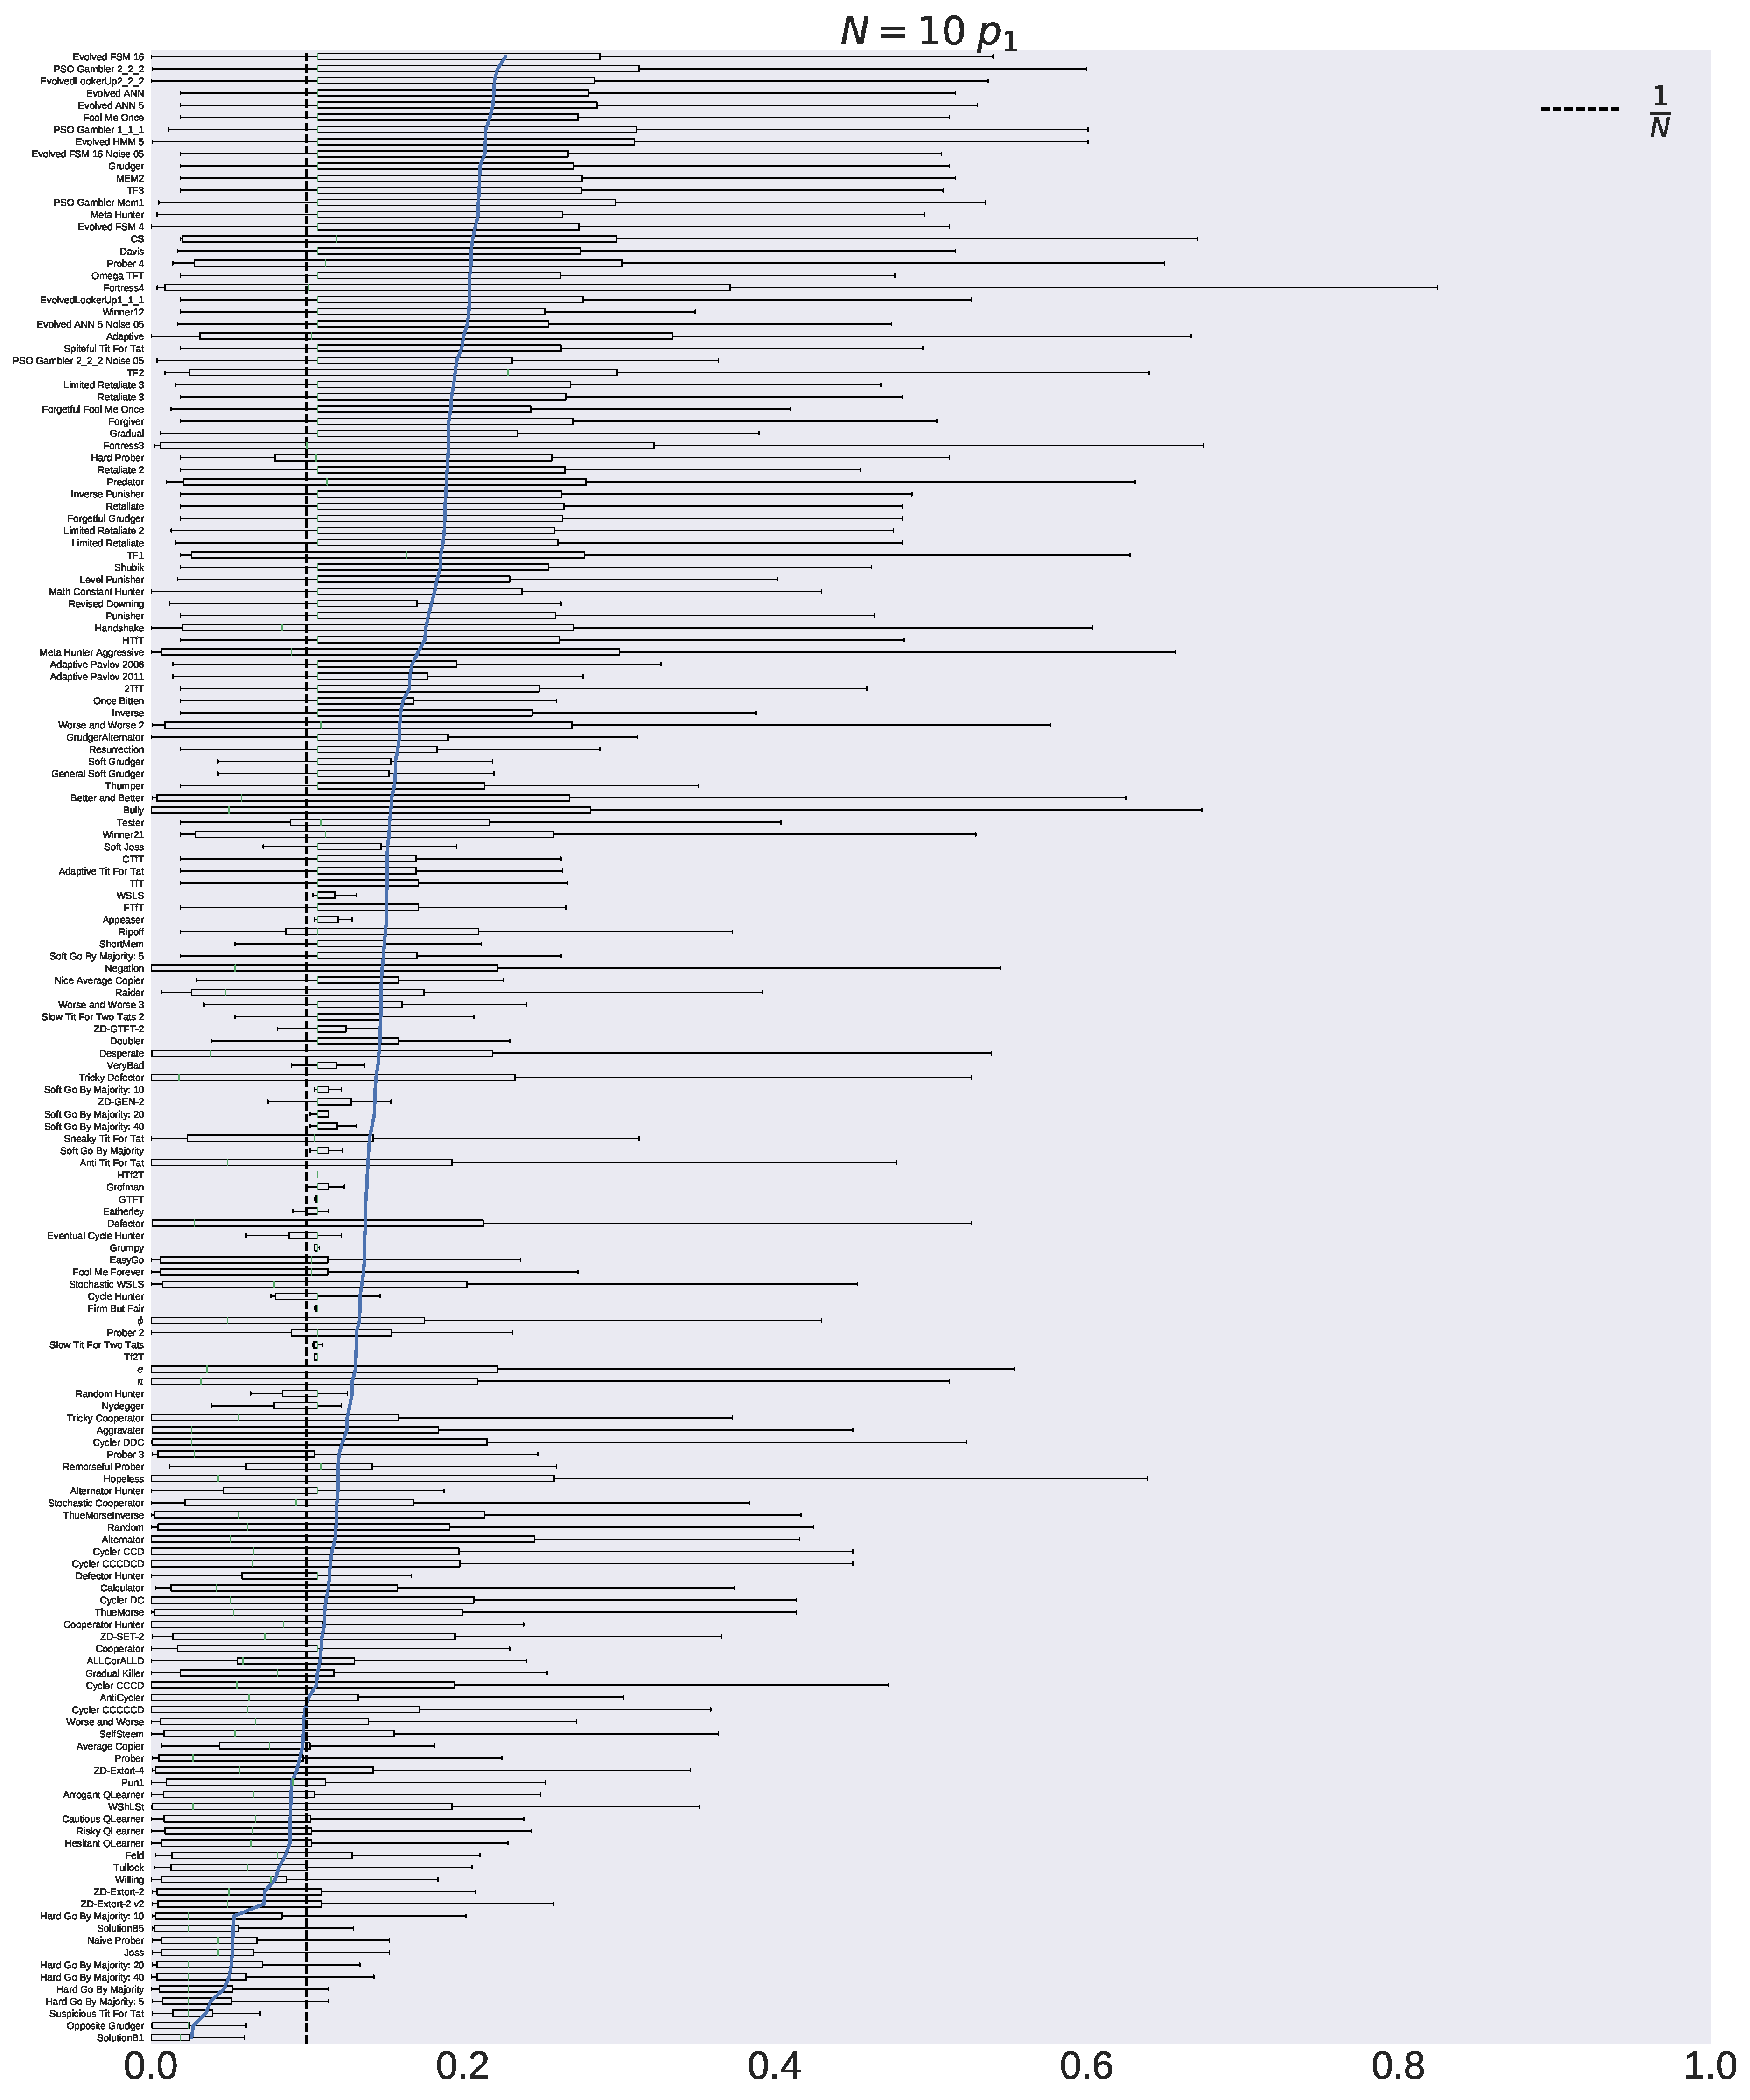
\includegraphics[width=\textwidth]{img/boxplot_10_invade.pdf}
    \caption{The fixation probabilities \(x_1\) for \(N=10\)}
\end{figure}

\begin{figure}[!hbtp]
    \centering
    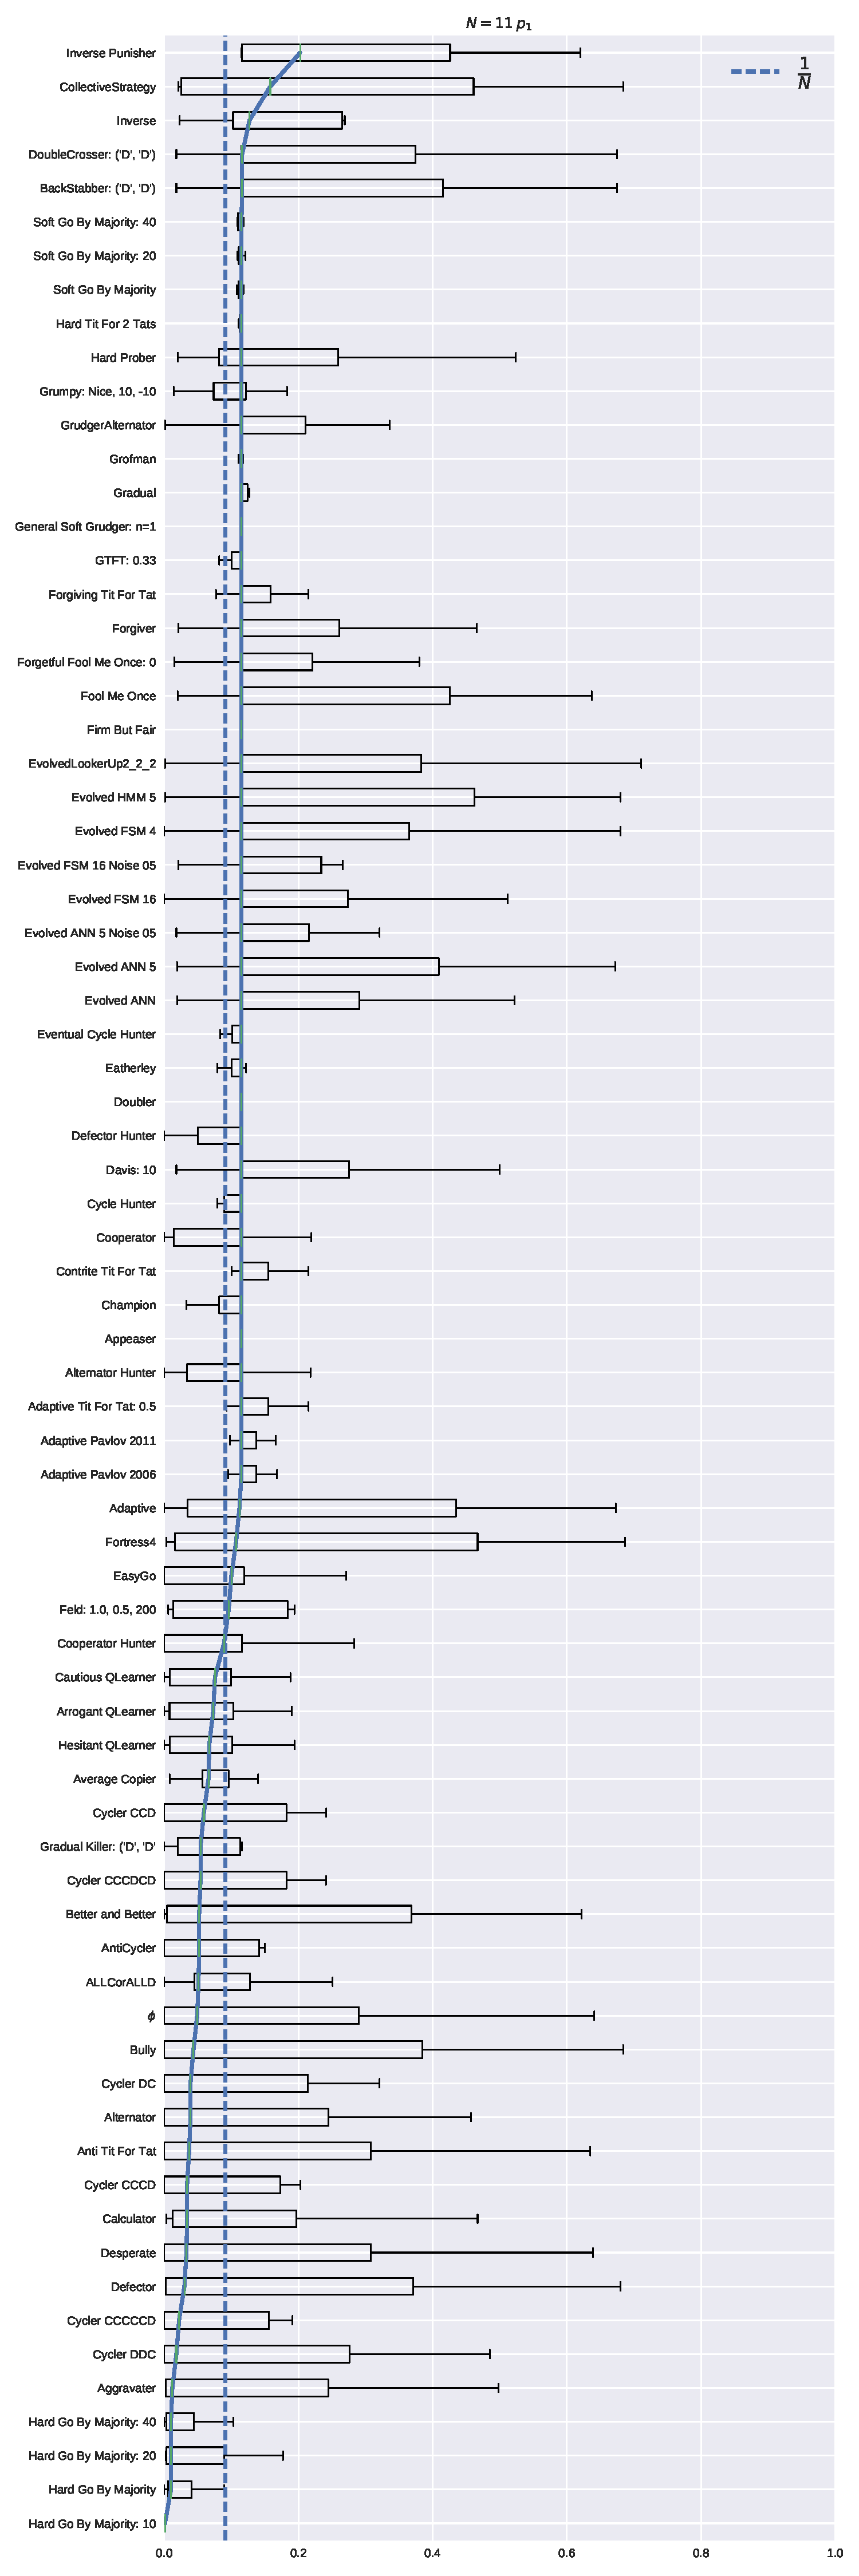
\includegraphics[width=\textwidth]{img/boxplot_11_invade.pdf}
    \caption{The fixation probabilities \(x_1\) for \(N=11\)}
\end{figure}

\begin{figure}[!hbtp]
    \centering
    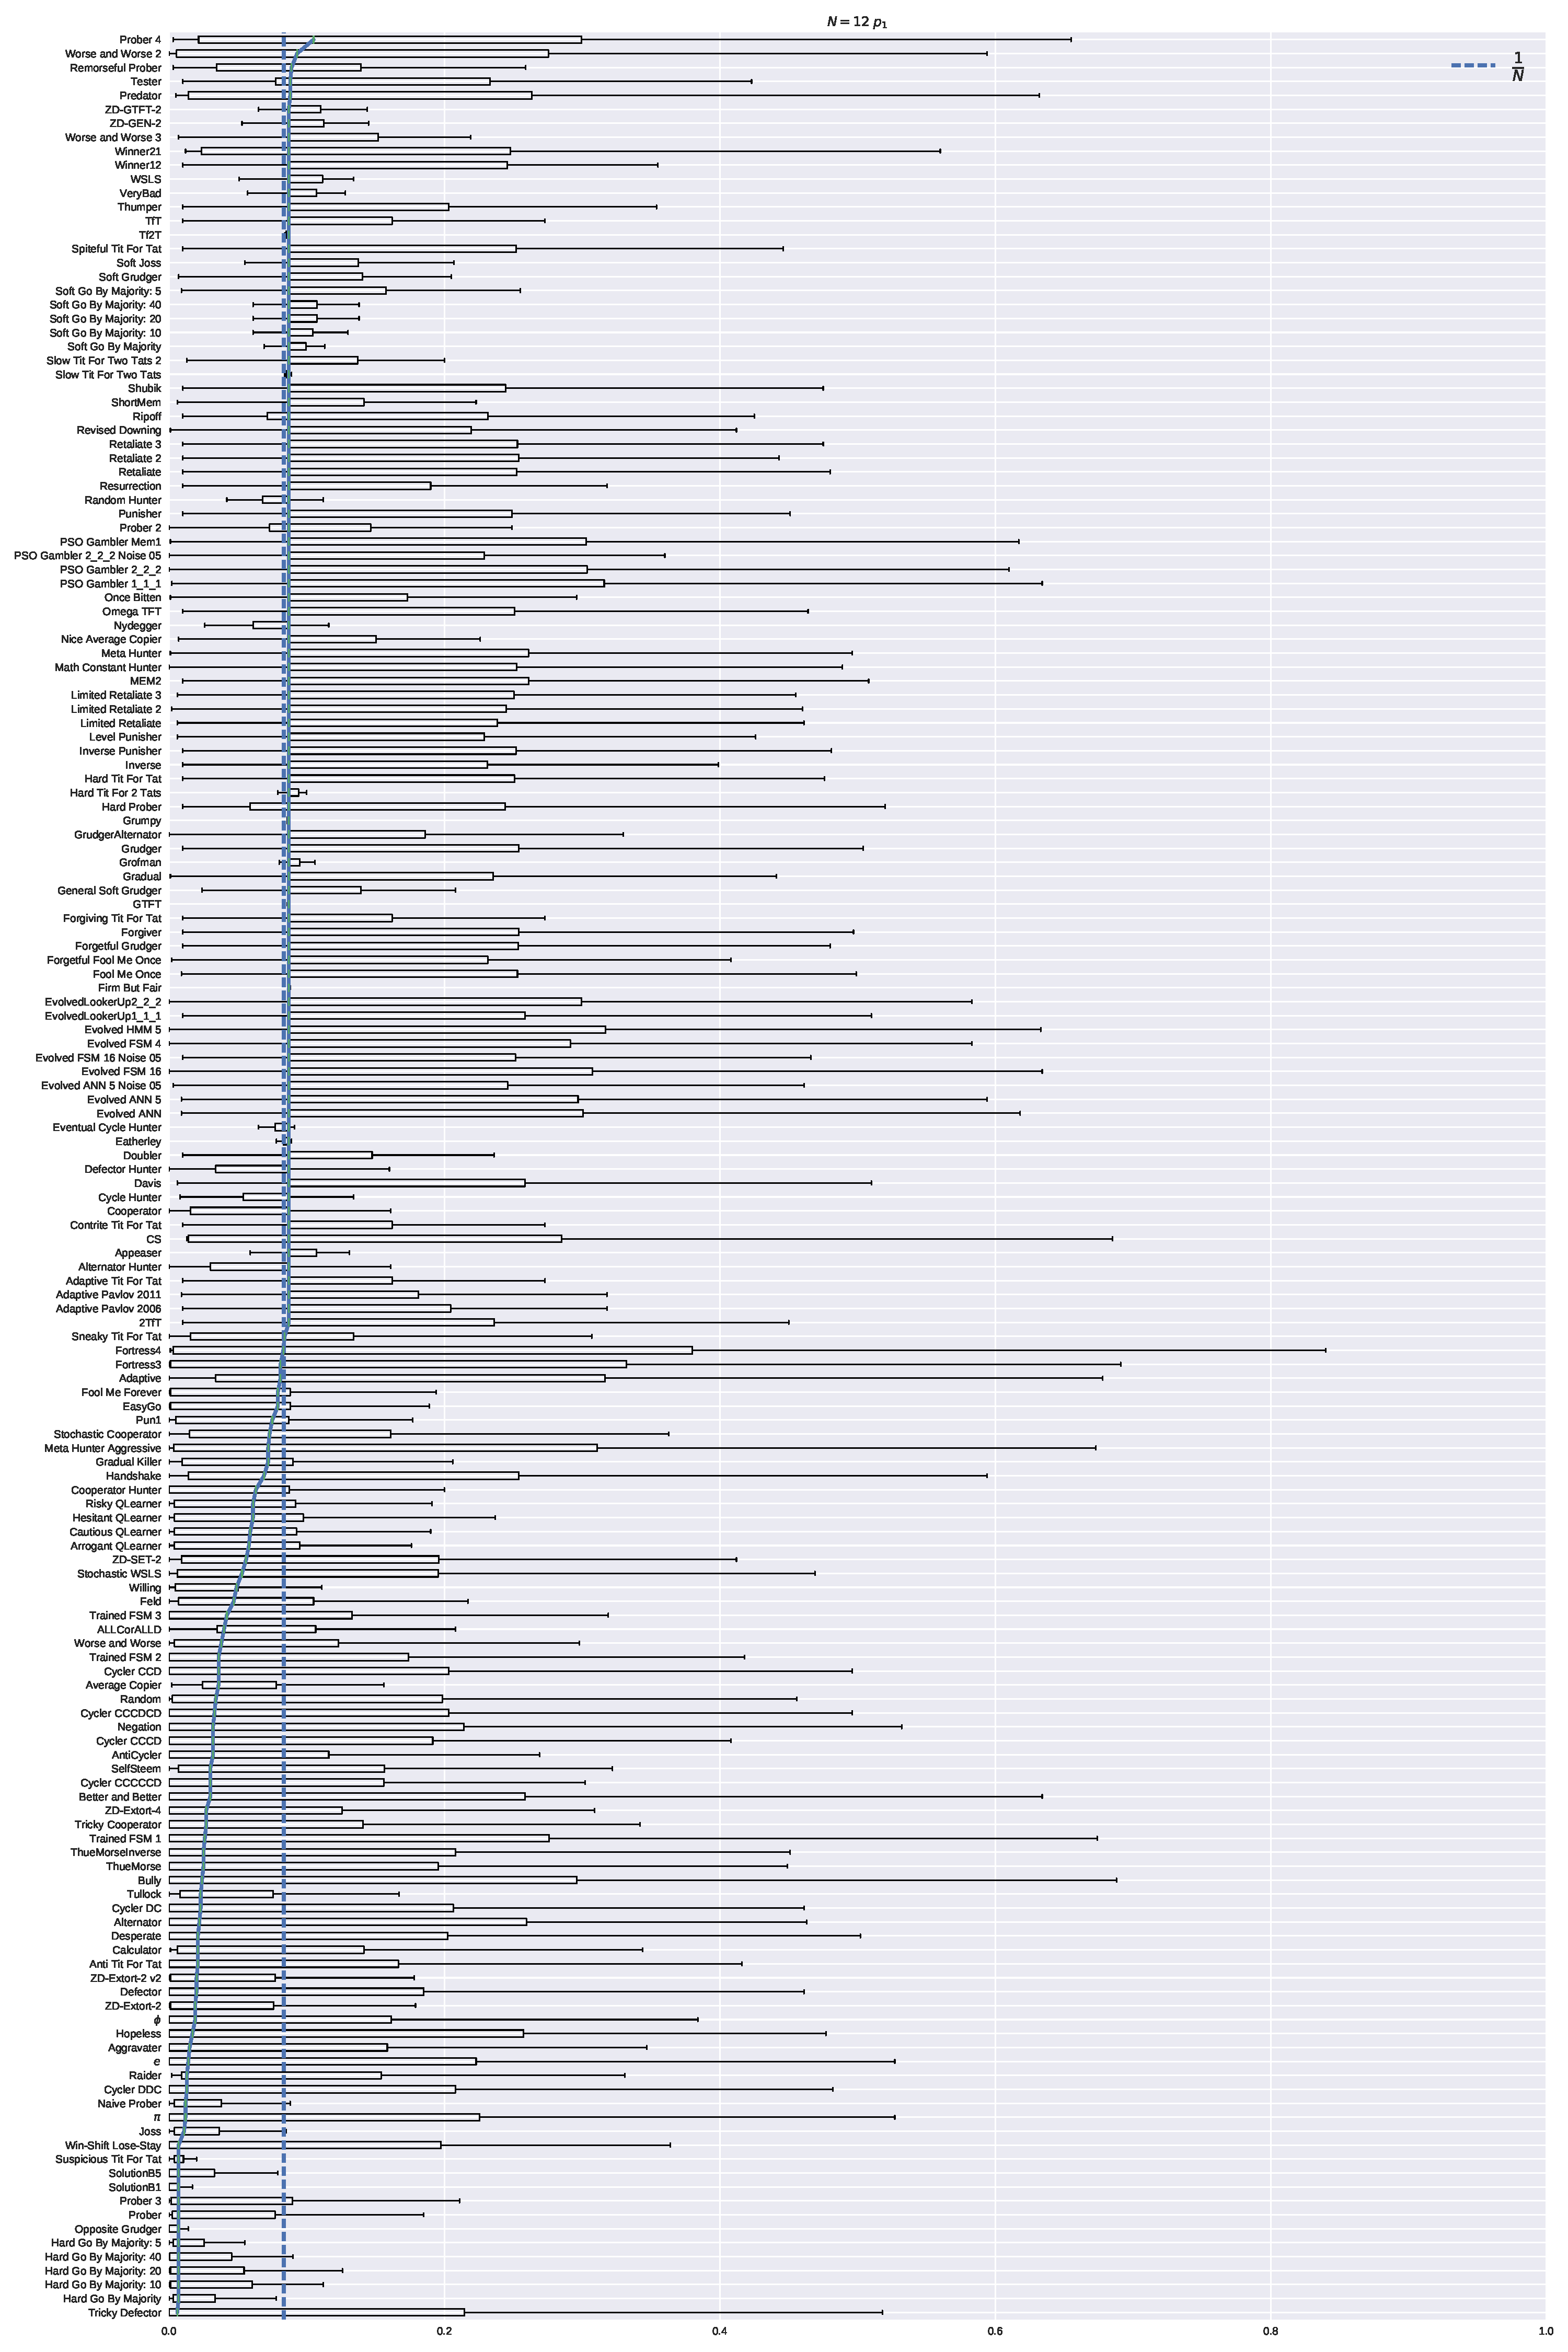
\includegraphics[width=\textwidth]{img/boxplot_12_invade.pdf}
    \caption{The fixation probabilities \(x_1\) for \(N=12\)}
\end{figure}

\begin{figure}[!hbtp]
    \centering
    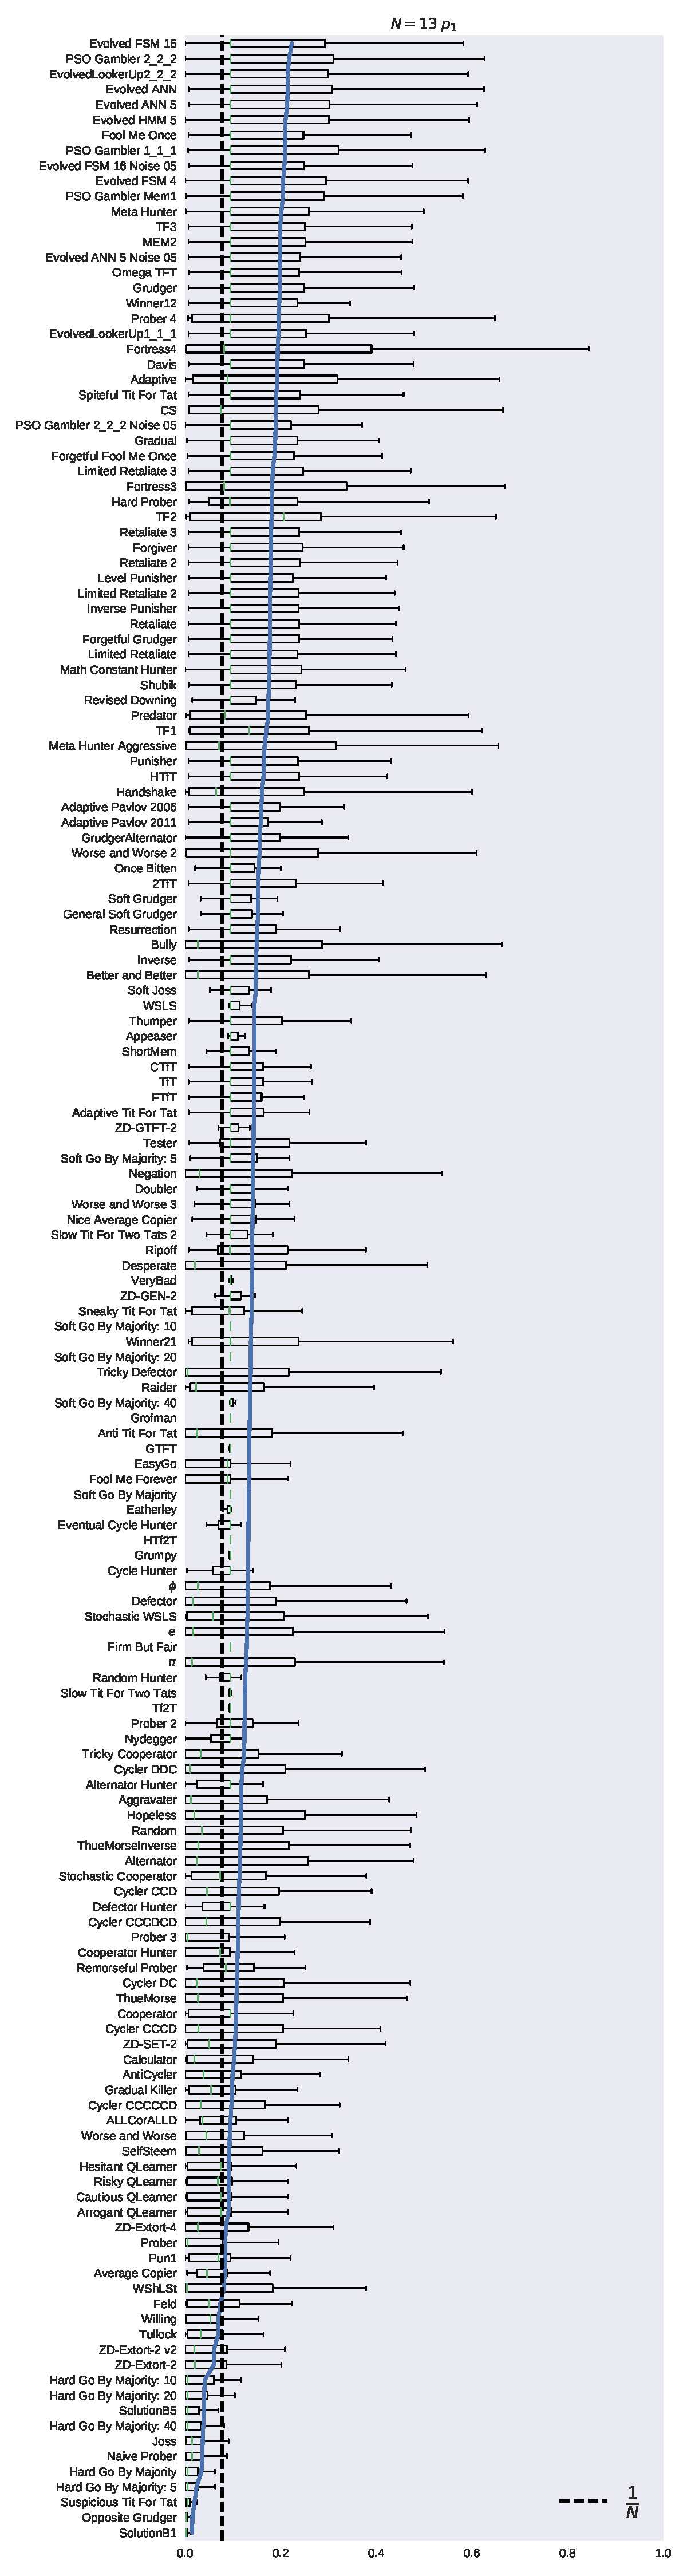
\includegraphics[width=\textwidth]{img/boxplot_13_invade.pdf}
    \caption{The fixation probabilities \(x_1\) for \(N=13\)}
\end{figure}

\begin{figure}[!hbtp]
    \centering
    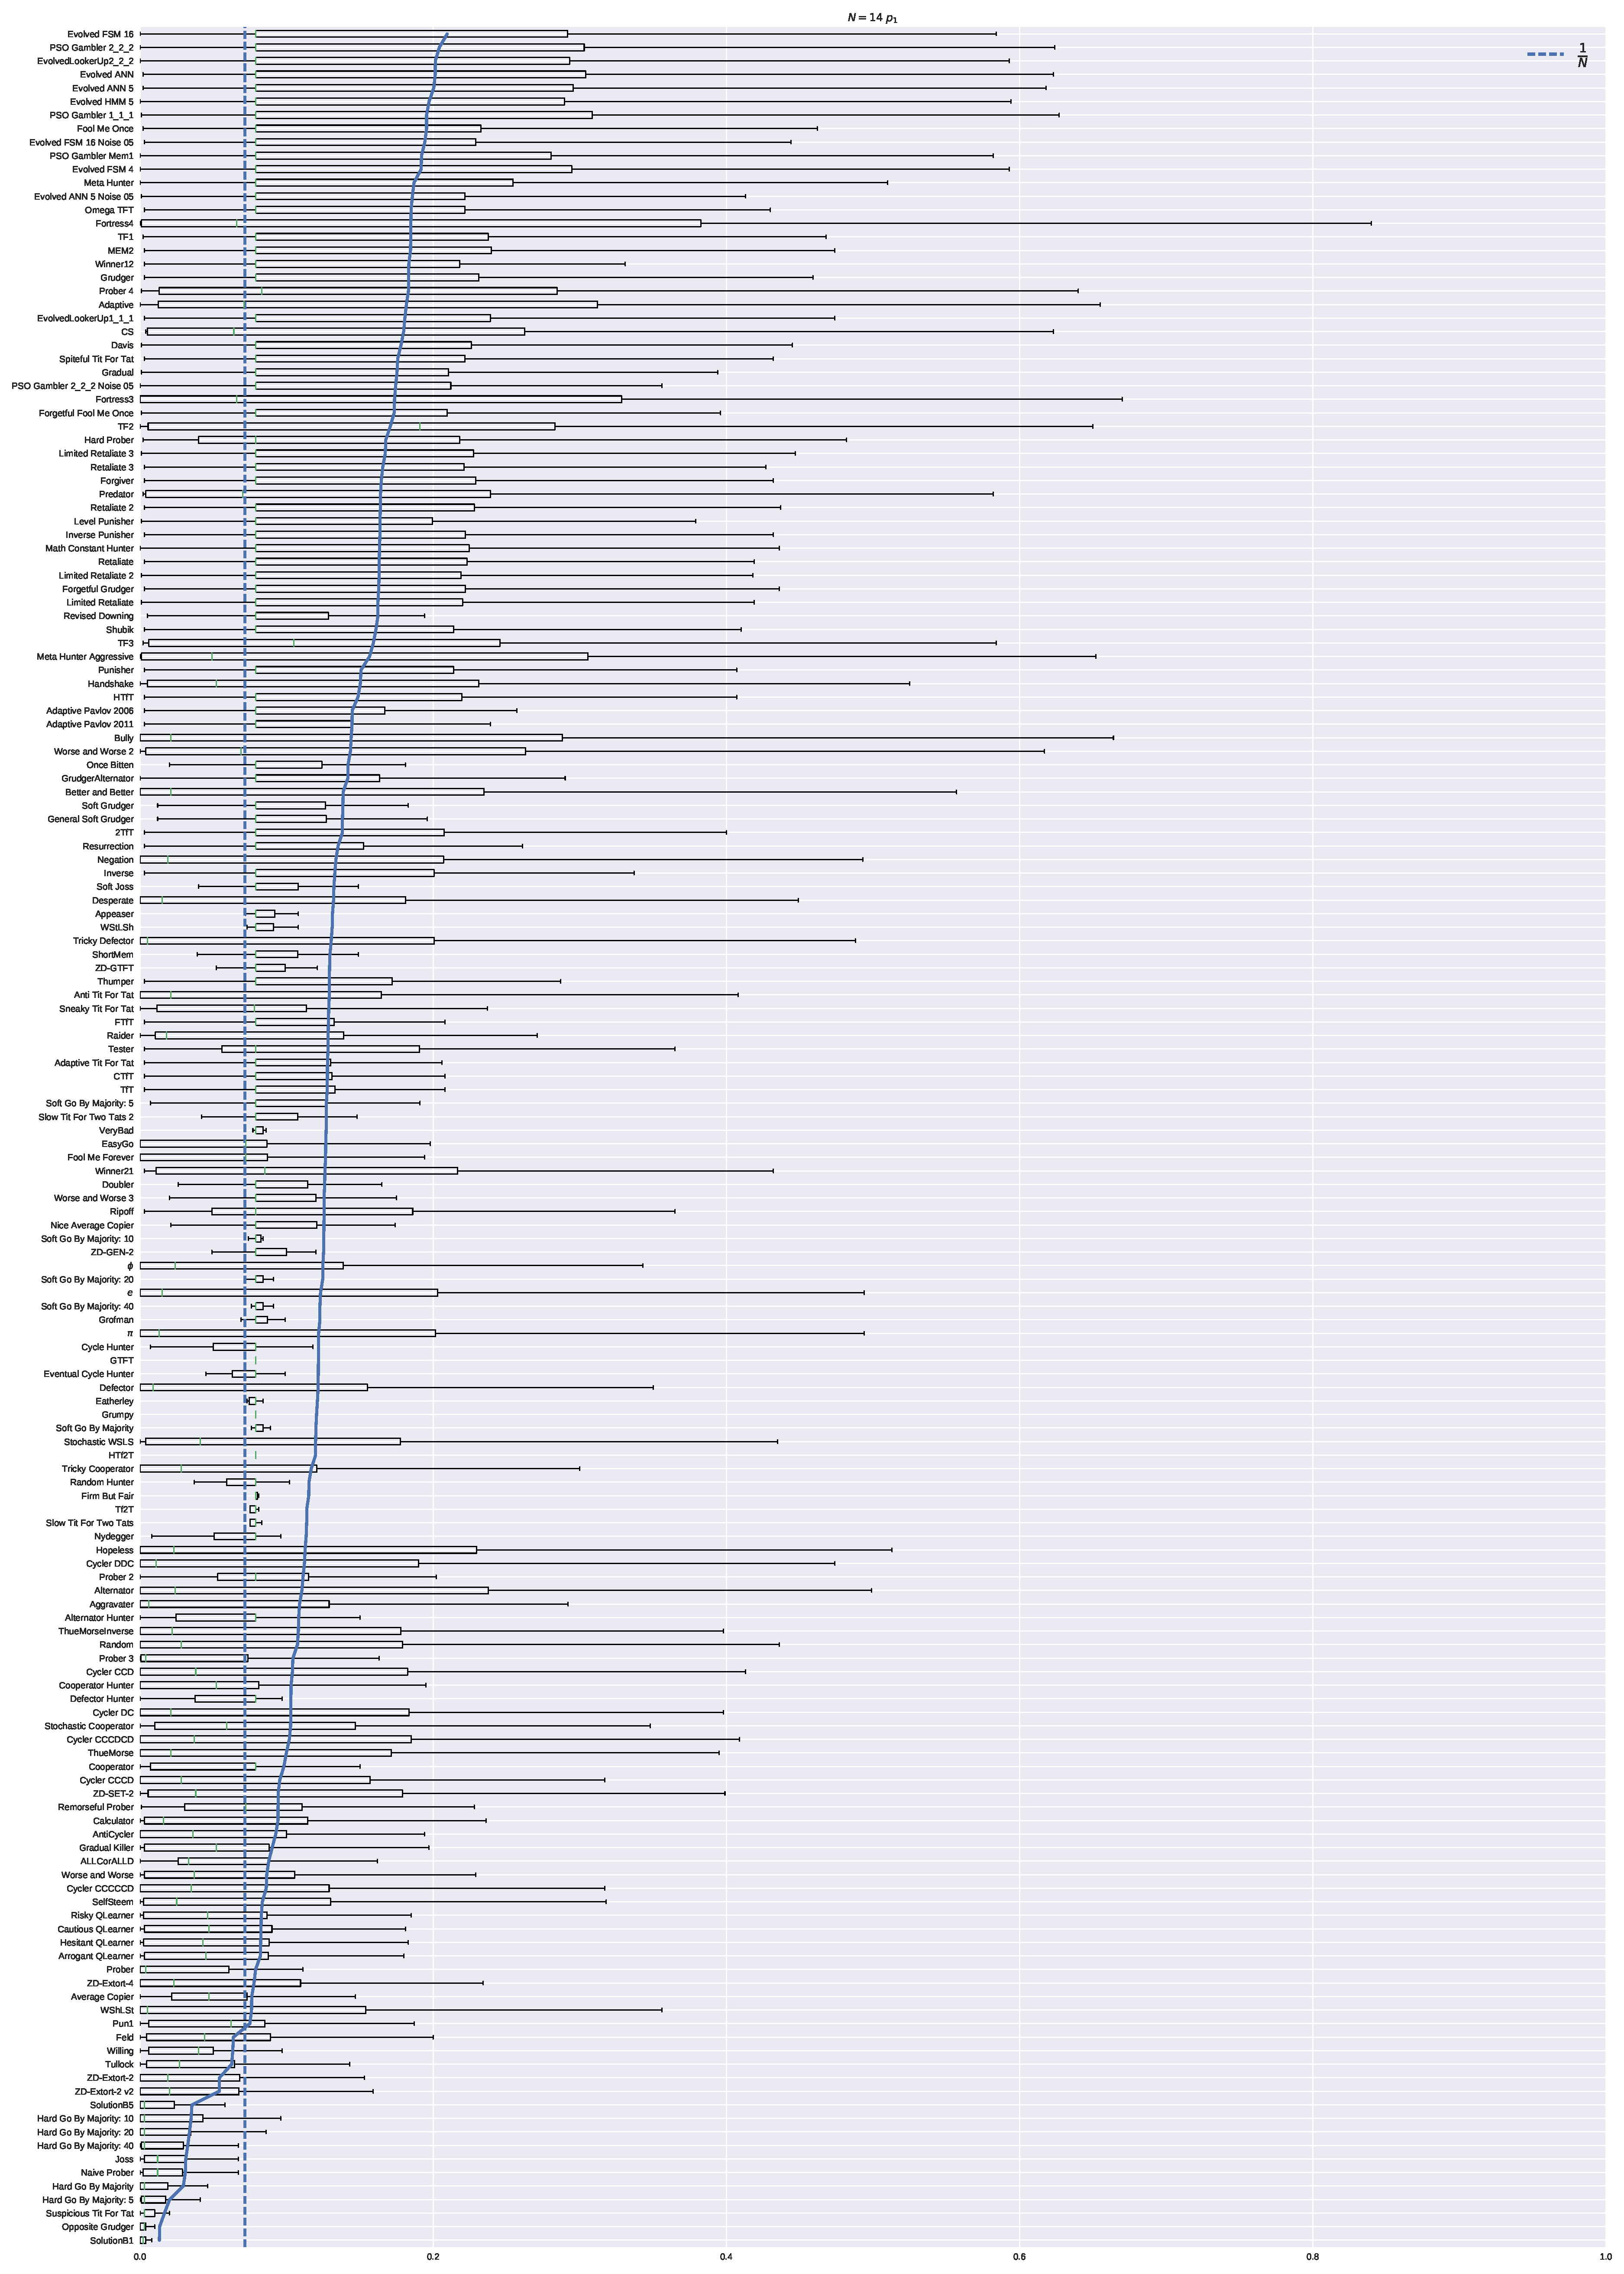
\includegraphics[width=\textwidth]{img/boxplot_14_invade.pdf}
    \caption{The fixation probabilities \(x_1\) for \(N=14\)}
    \label{invasion-14}
\end{figure}


\begin{figure}[!hbtp]
    \centering
    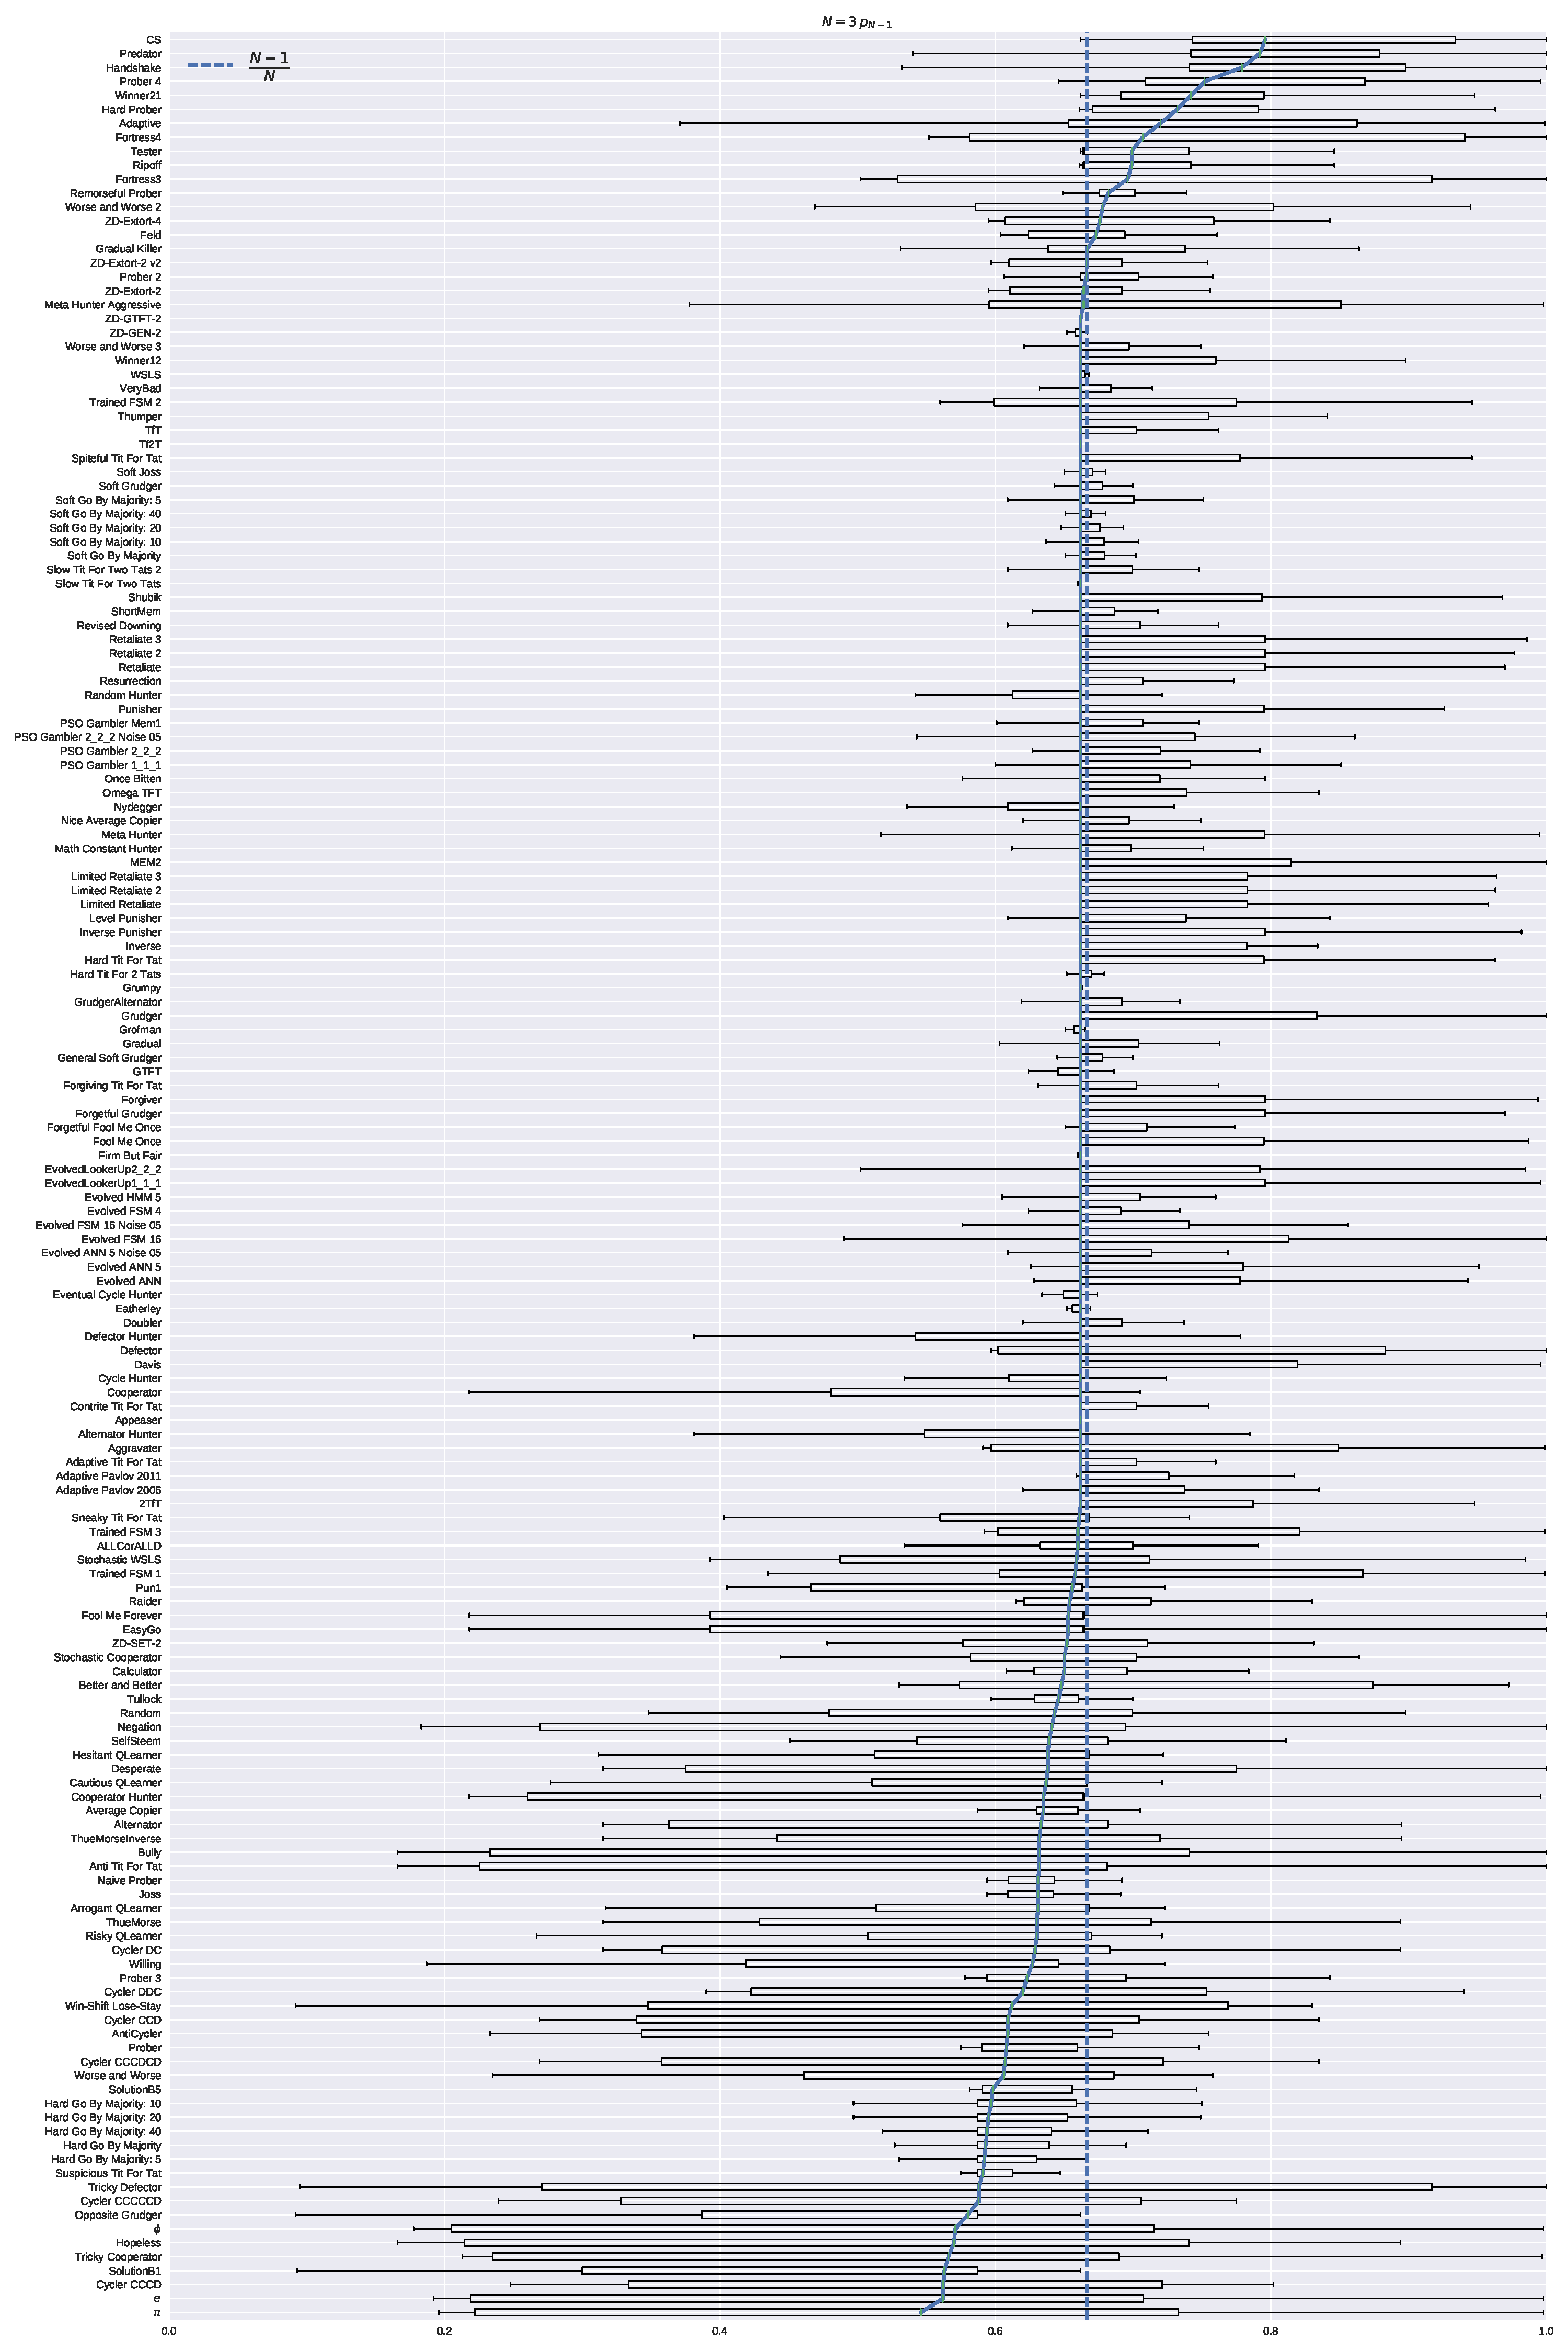
\includegraphics[width=\textwidth]{img/boxplot_3_resist.pdf}
    \caption{The fixation probabilities \(x_{N-1}\) for \(N=3\)}
    \label{resistance-3}
\end{figure}

\begin{figure}[!hbtp]
    \centering
    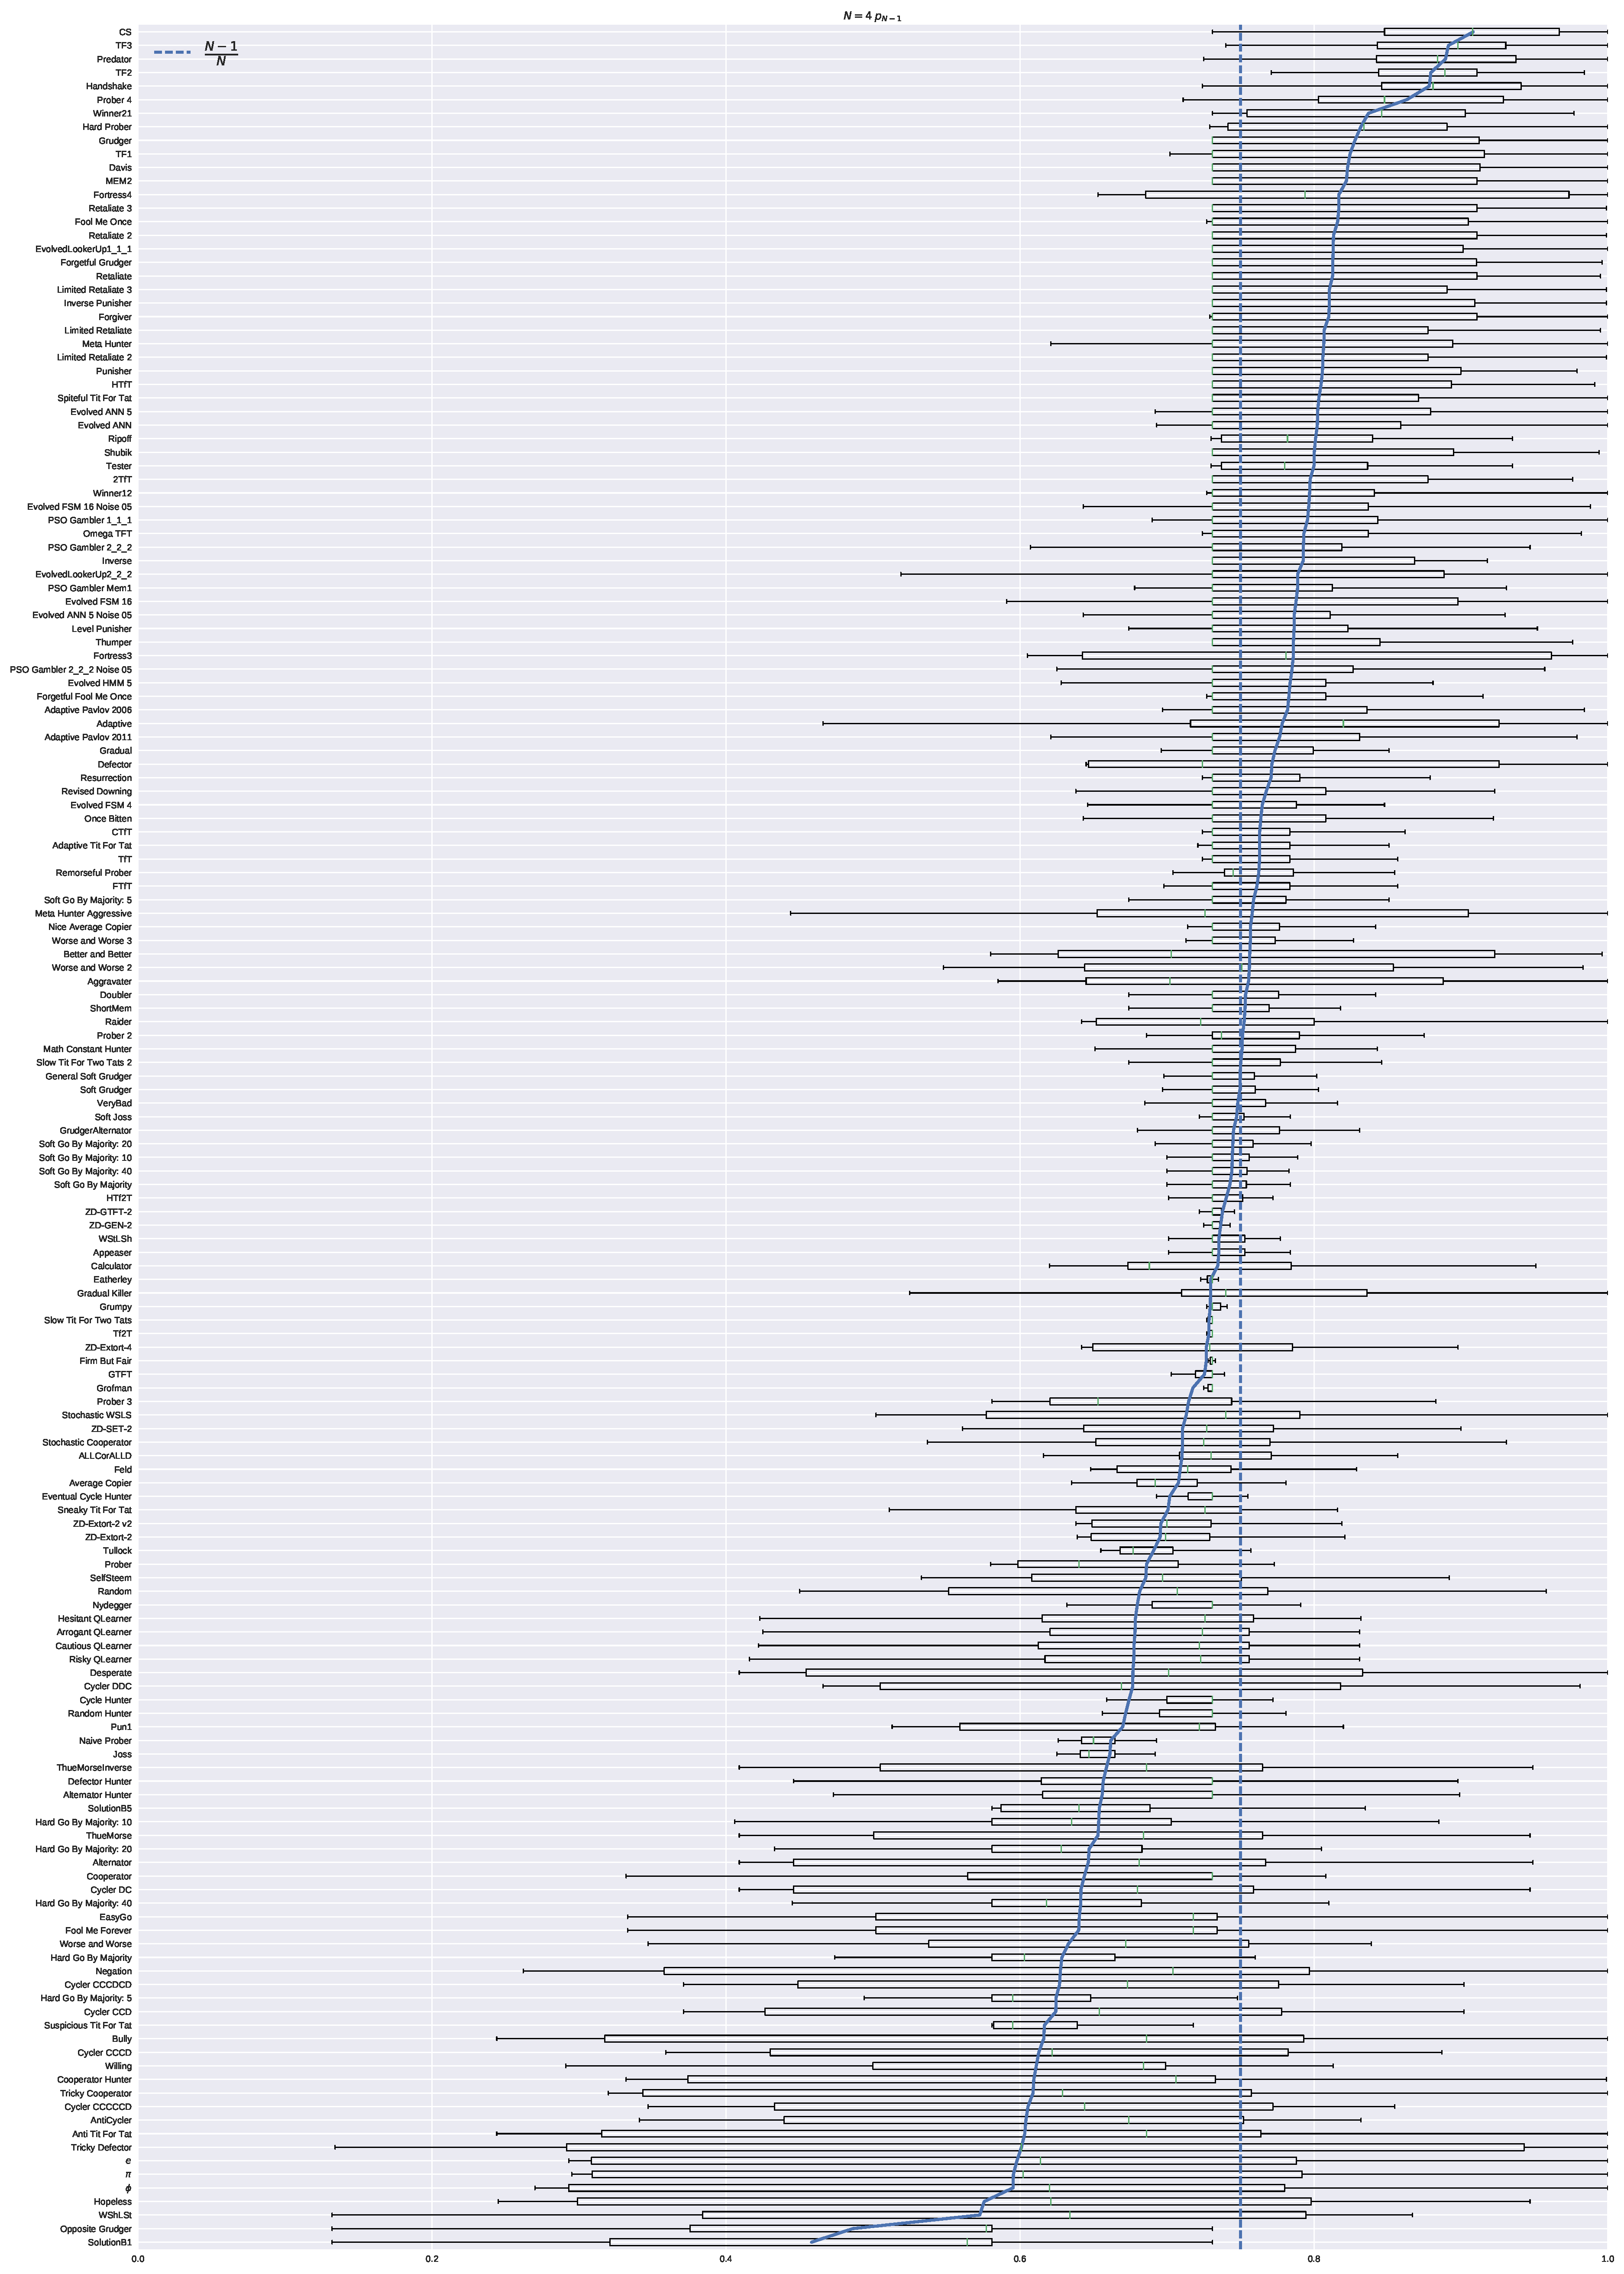
\includegraphics[width=\textwidth]{img/boxplot_4_resist.pdf}
    \caption{The fixation probabilities \(x_{N-1}\) for \(N=4\)}
\end{figure}

\begin{figure}[!hbtp]
    \centering
    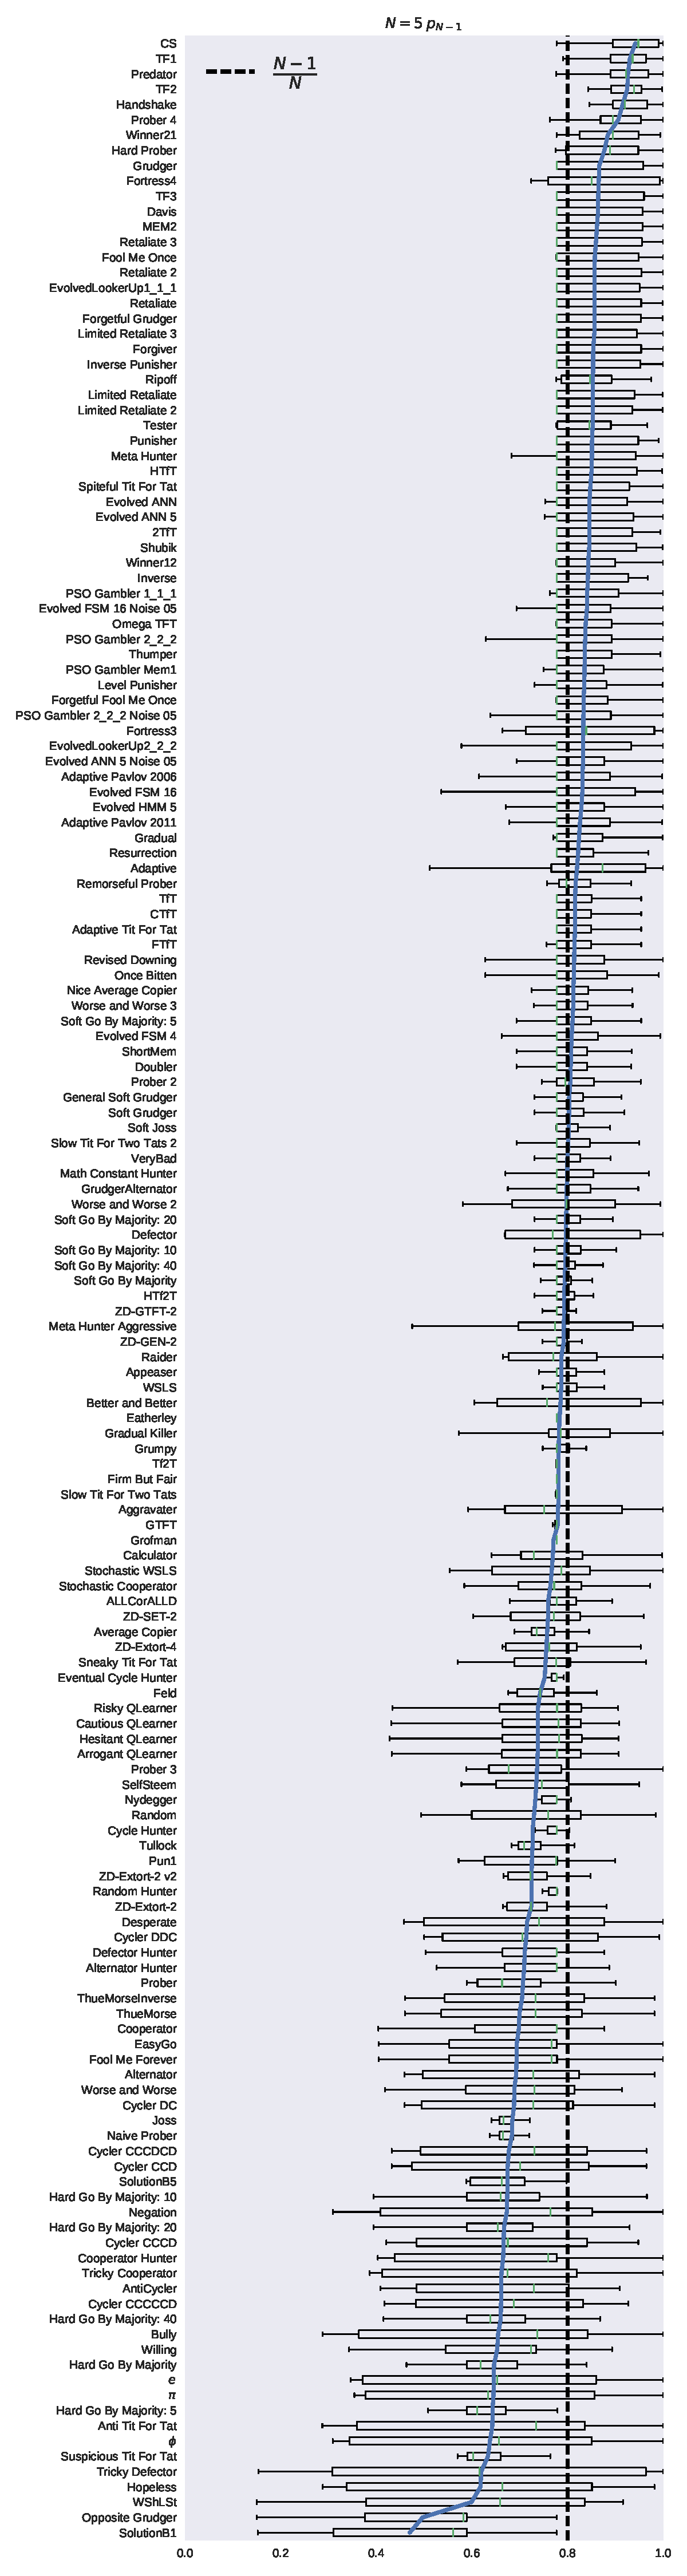
\includegraphics[width=\textwidth]{img/boxplot_5_resist.pdf}
    \caption{The fixation probabilities \(x_{N-1}\) for \(N=5\)}
\end{figure}

\begin{figure}[!hbtp]
    \centering
    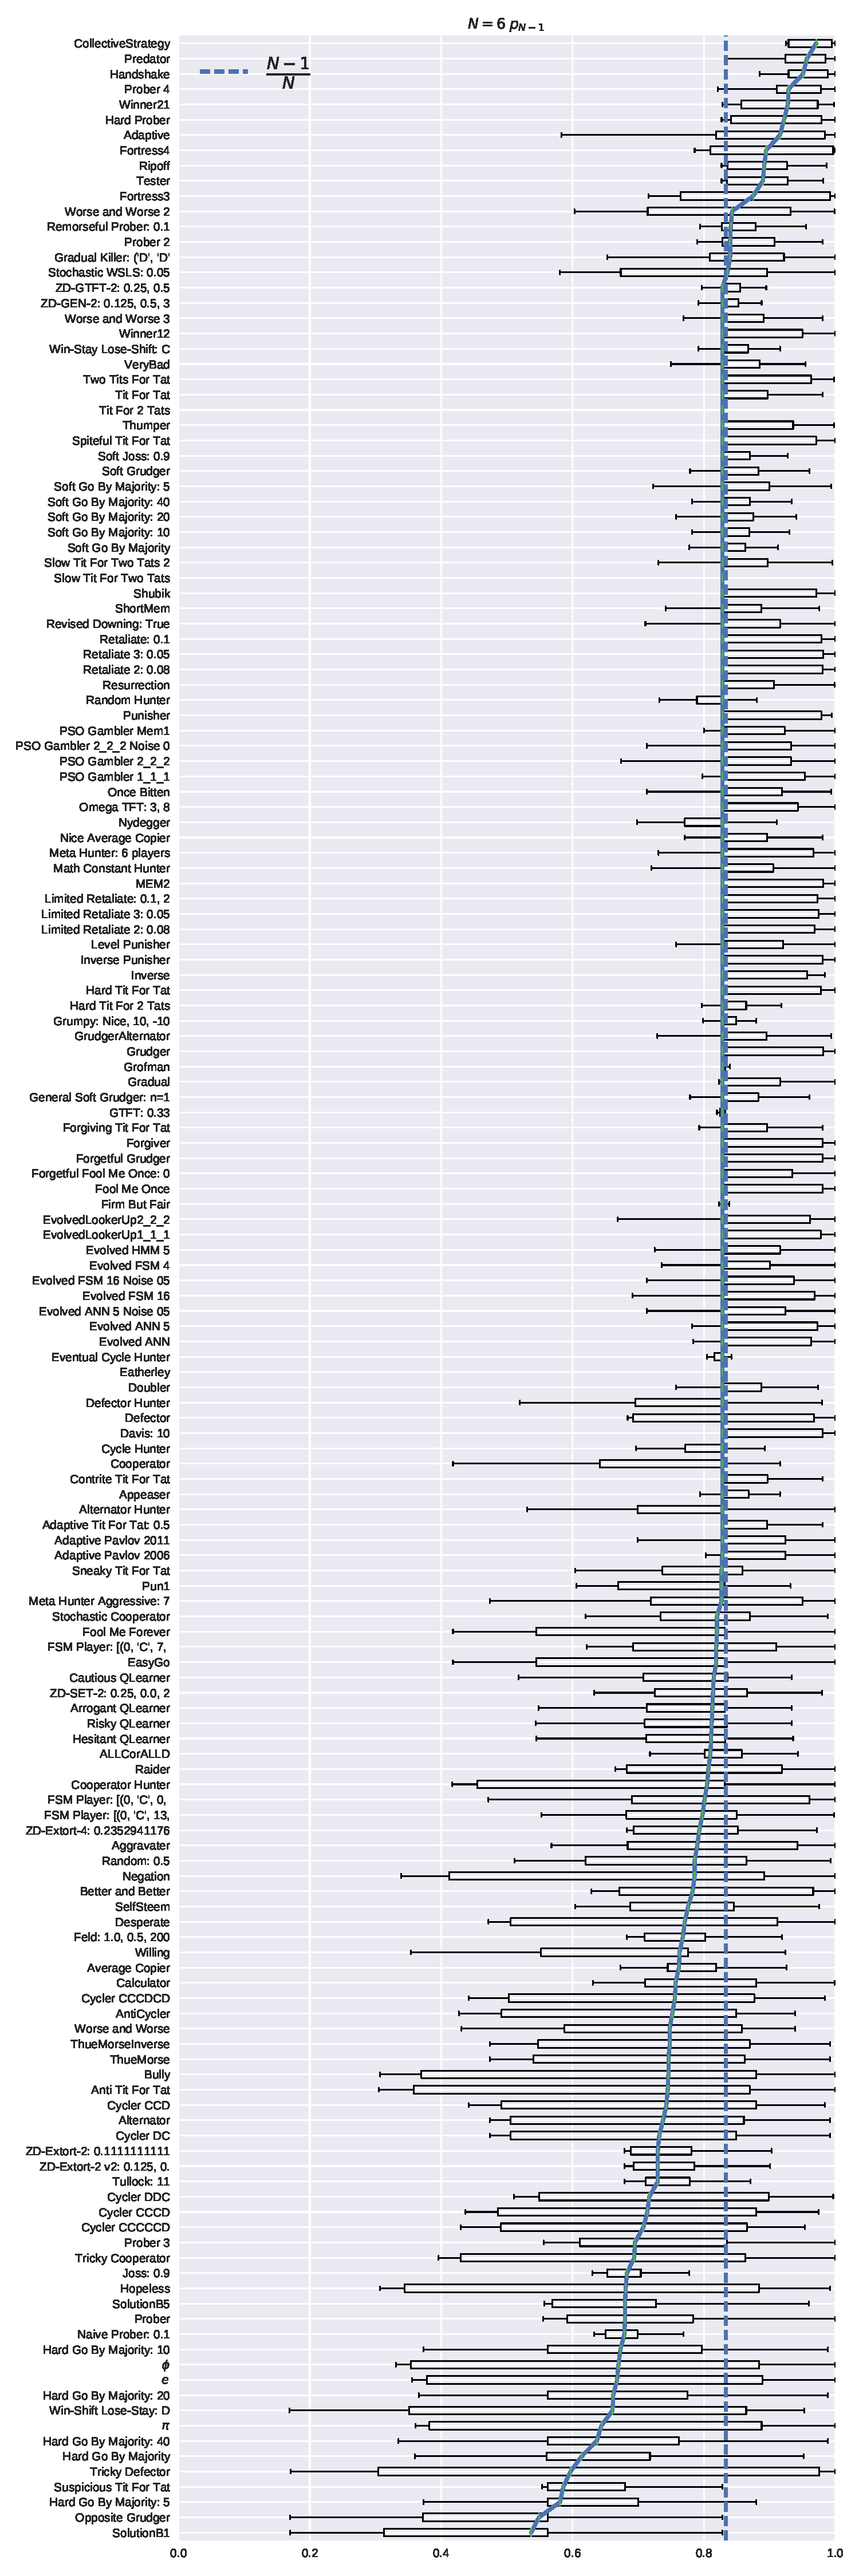
\includegraphics[width=\textwidth]{img/boxplot_6_resist.pdf}
    \caption{The fixation probabilities \(x_{N-1}\) for \(N=6\)}
\end{figure}

\begin{figure}[!hbtp]
    \centering
    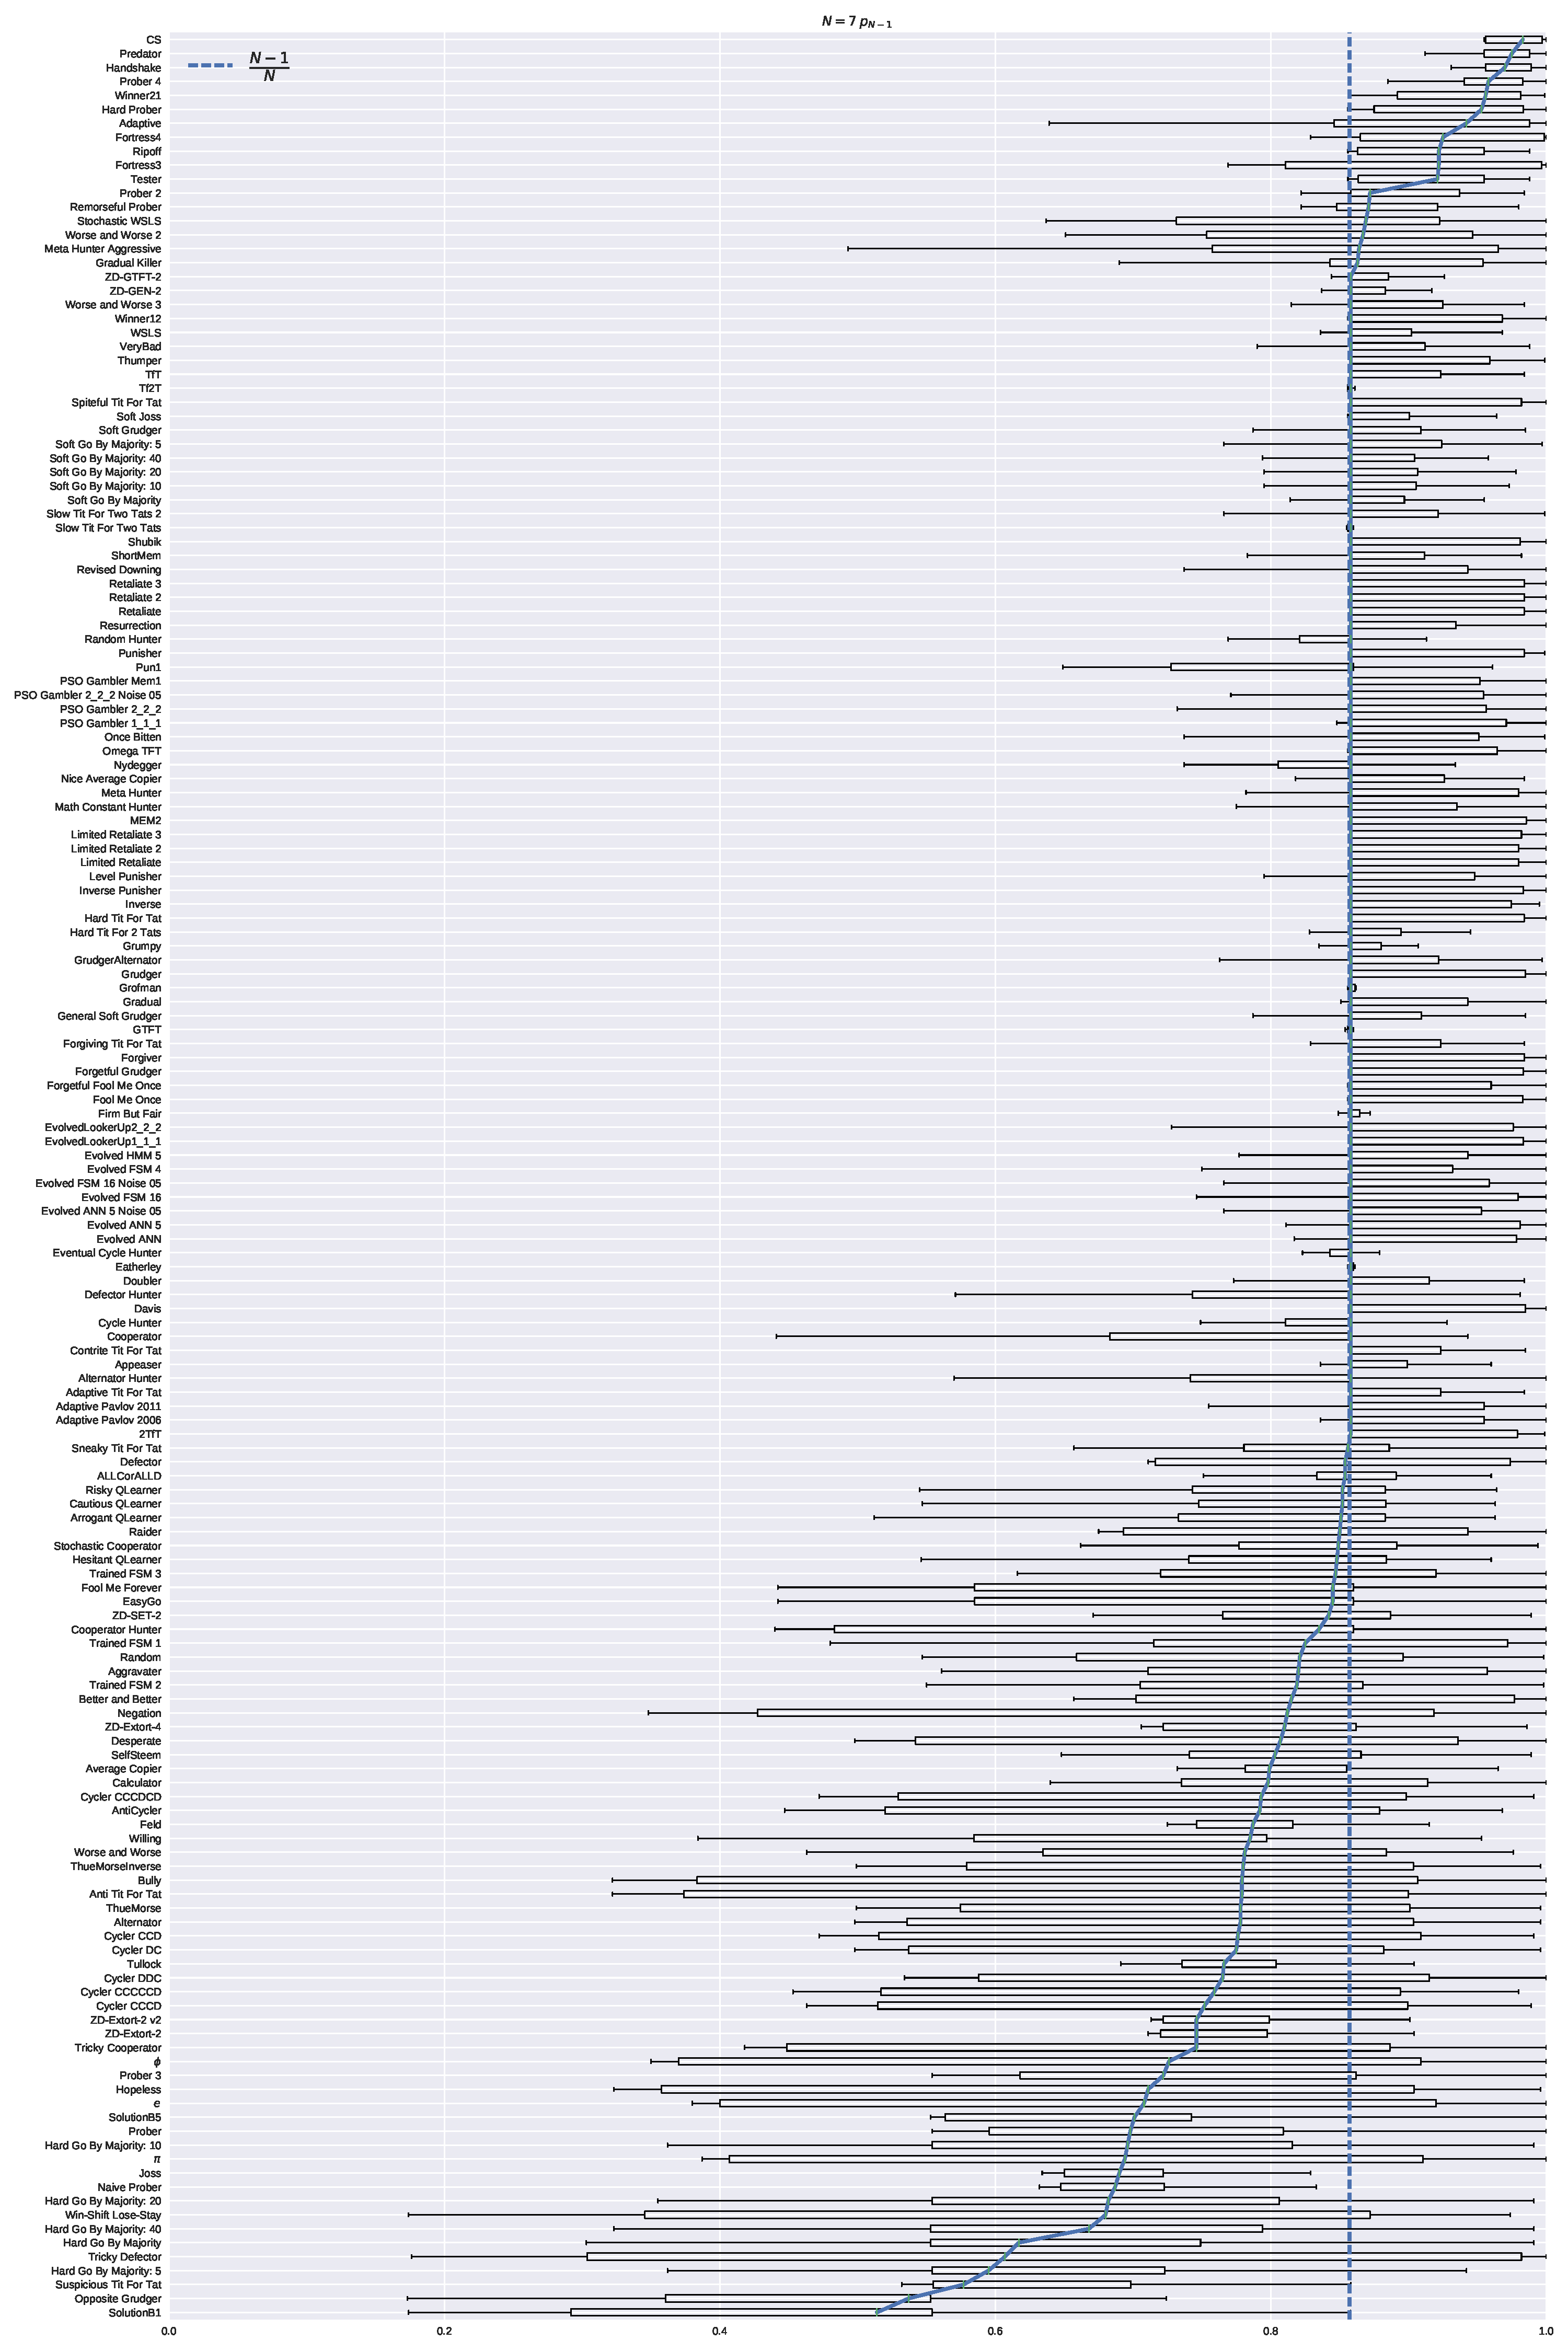
\includegraphics[width=\textwidth]{img/boxplot_7_resist.pdf}
    \caption{The fixation probabilities \(x_{N-1}\) for \(N=7\)}
\end{figure}

\begin{figure}[!hbtp]
    \centering
    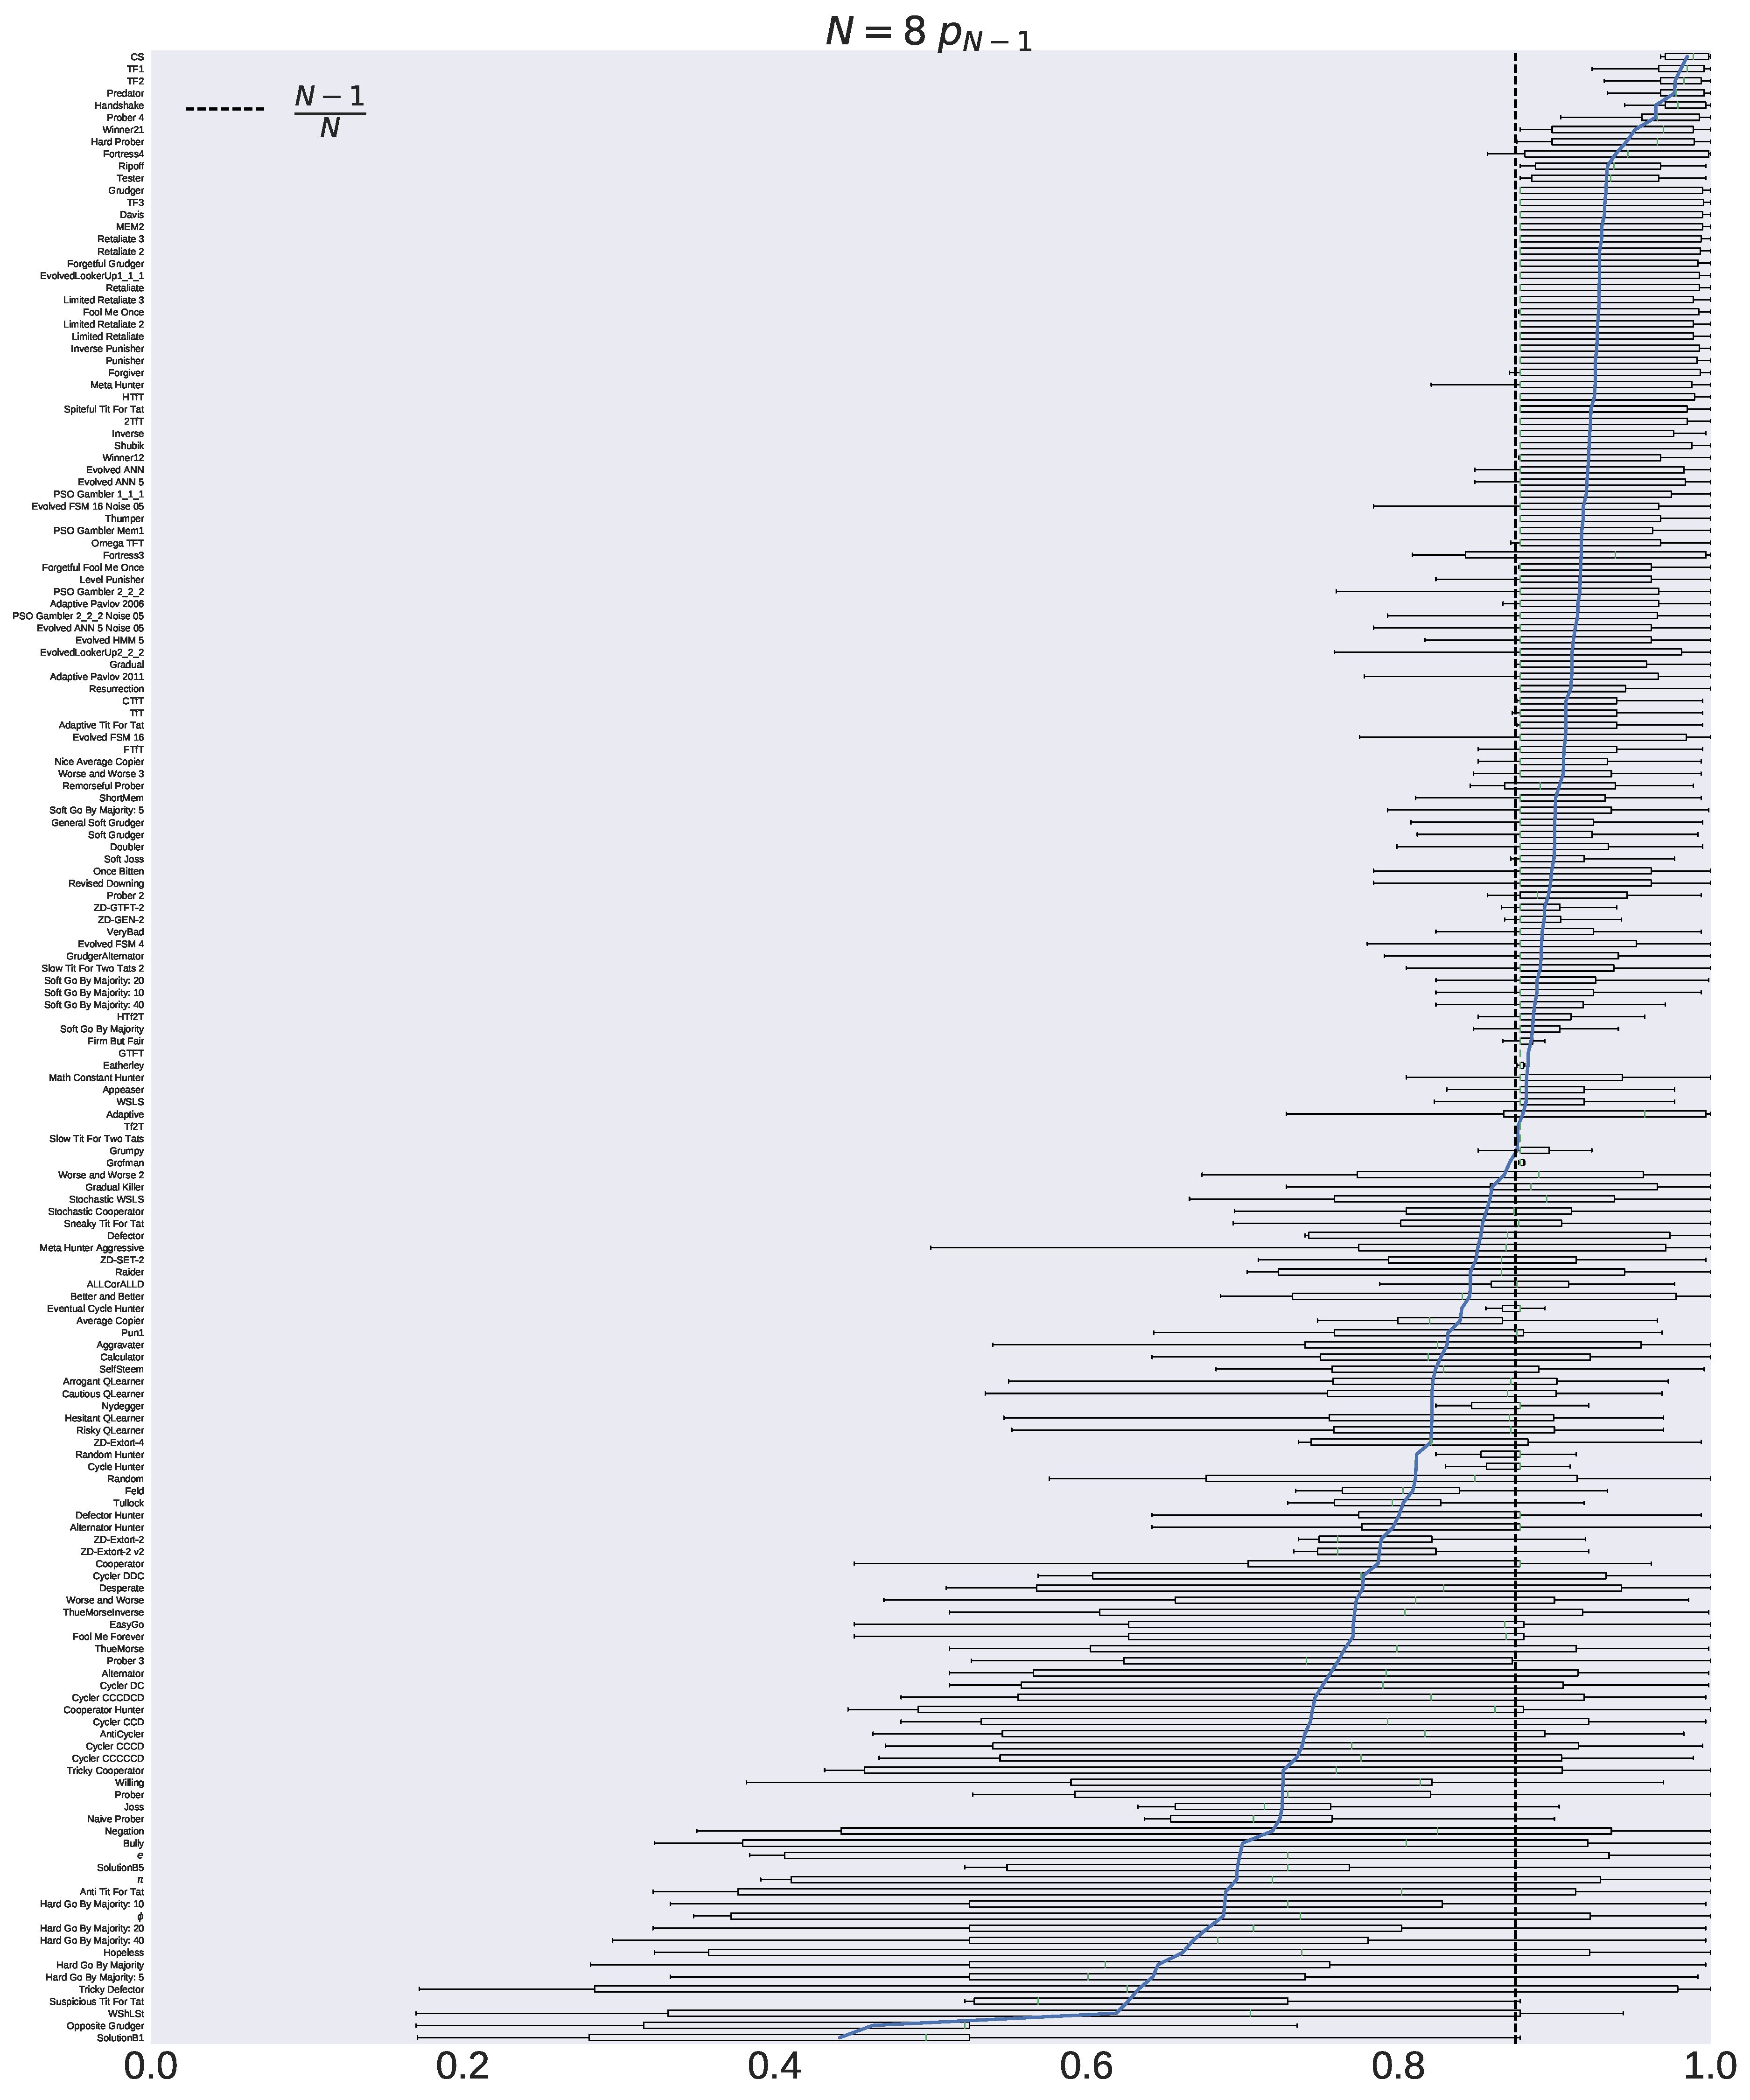
\includegraphics[width=\textwidth]{img/boxplot_8_resist.pdf}
    \caption{The fixation probabilities \(x_{N-1}\) for \(N=8\)}
\end{figure}

\begin{figure}[!hbtp]
    \centering
    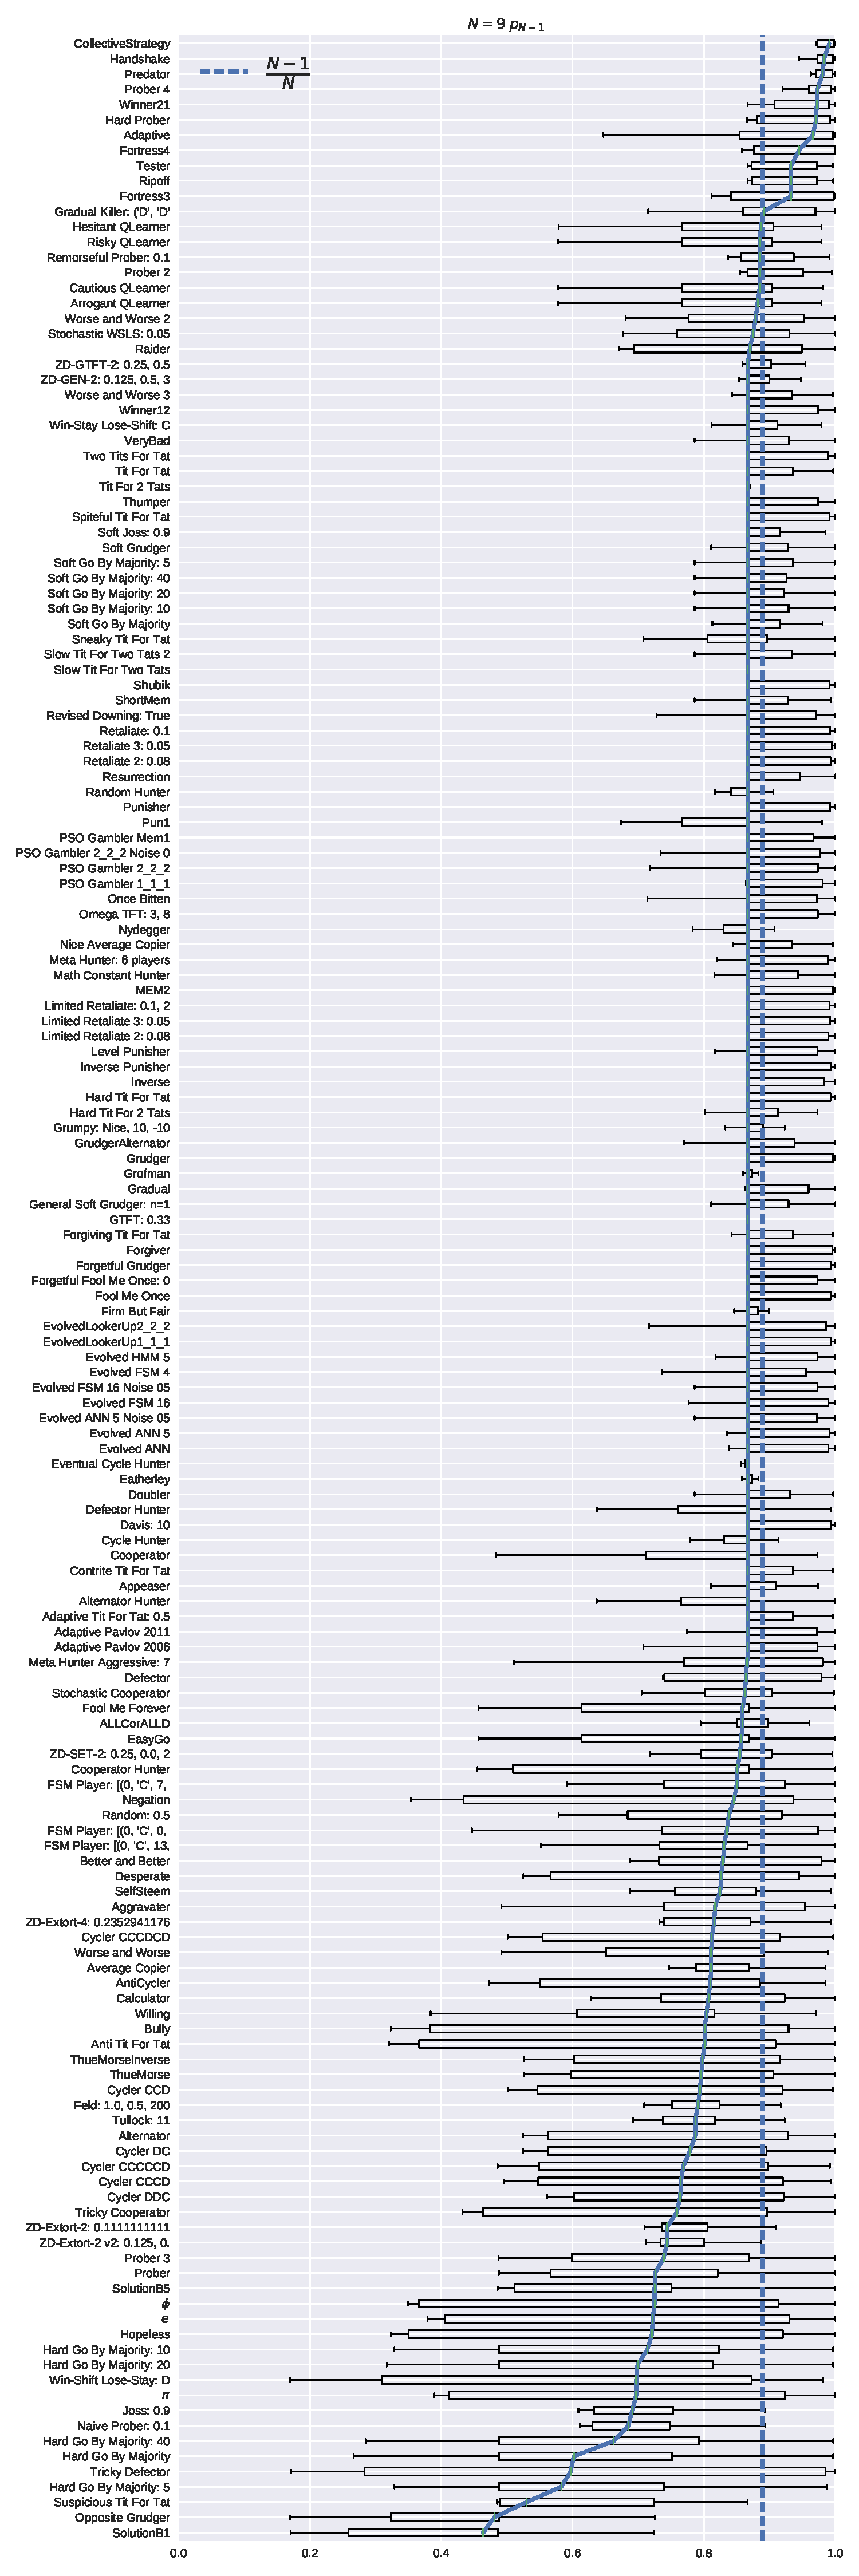
\includegraphics[width=\textwidth]{img/boxplot_9_resist.pdf}
    \caption{The fixation probabilities \(x_{N-1}\) for \(N=9\)}
\end{figure}

\begin{figure}[!hbtp]
    \centering
    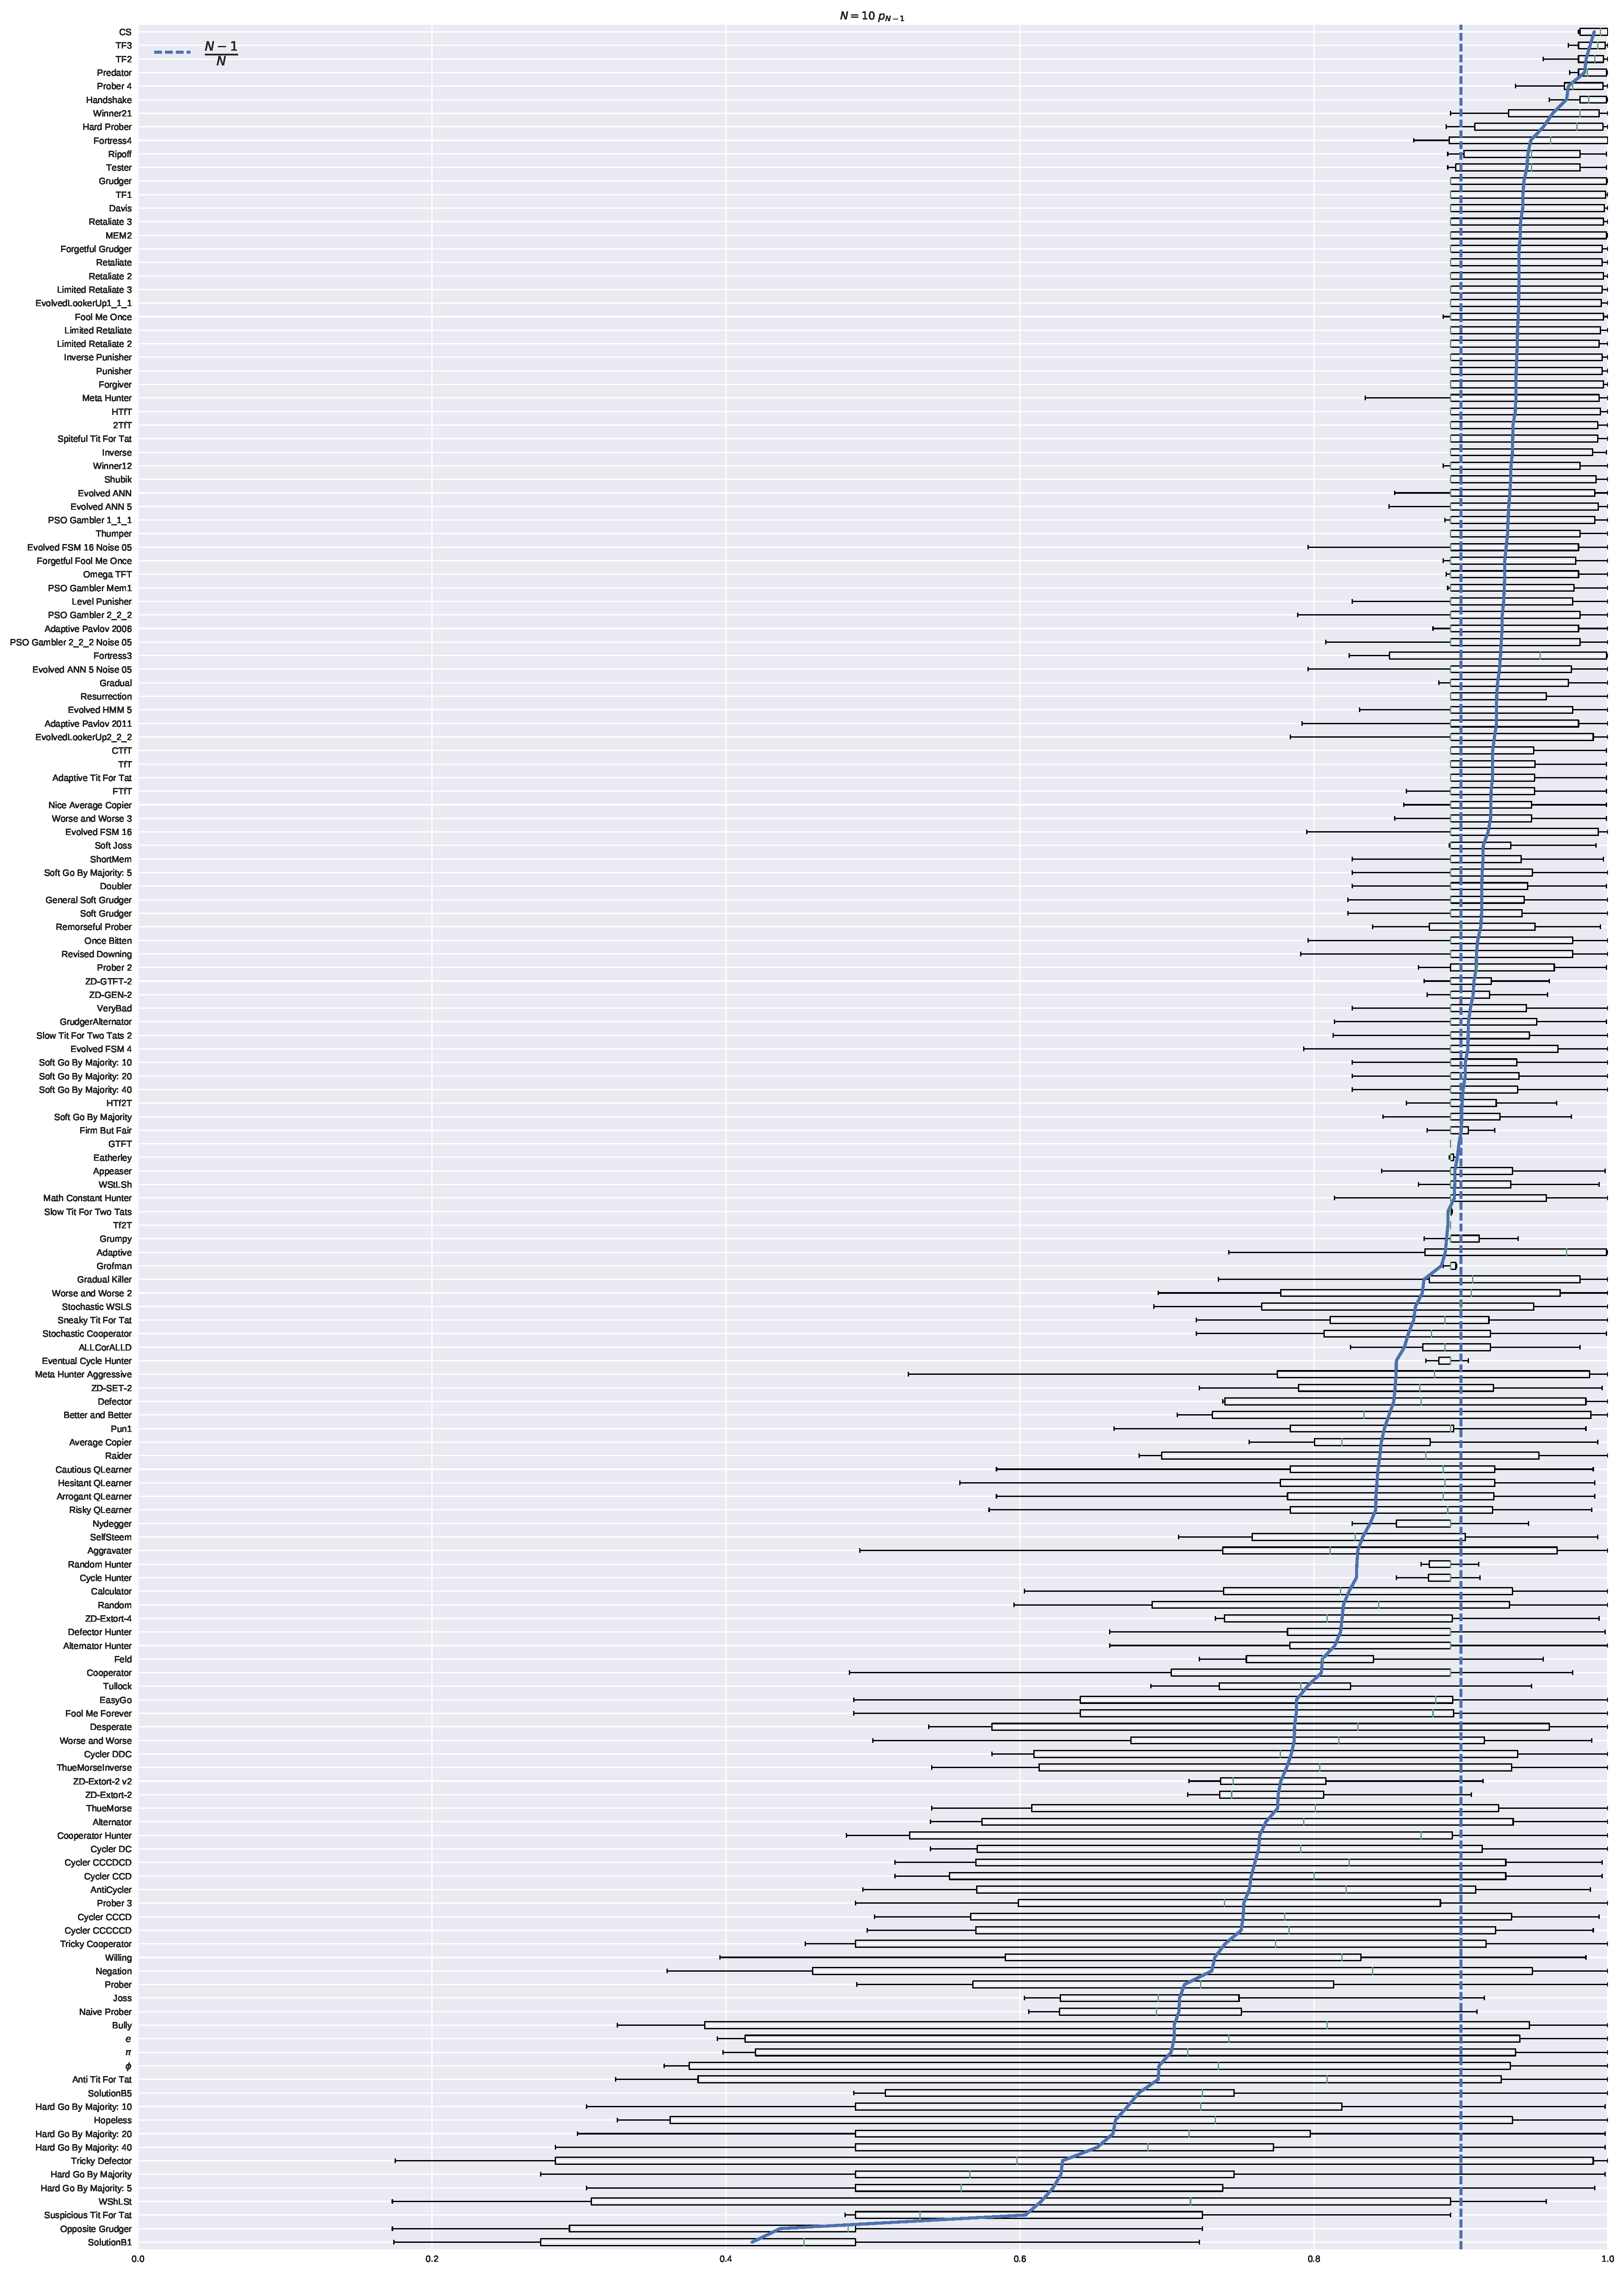
\includegraphics[width=\textwidth]{img/boxplot_10_resist.pdf}
    \caption{The fixation probabilities \(x_{N-1}\) for \(N=10\)}
\end{figure}

\begin{figure}[!hbtp]
    \centering
    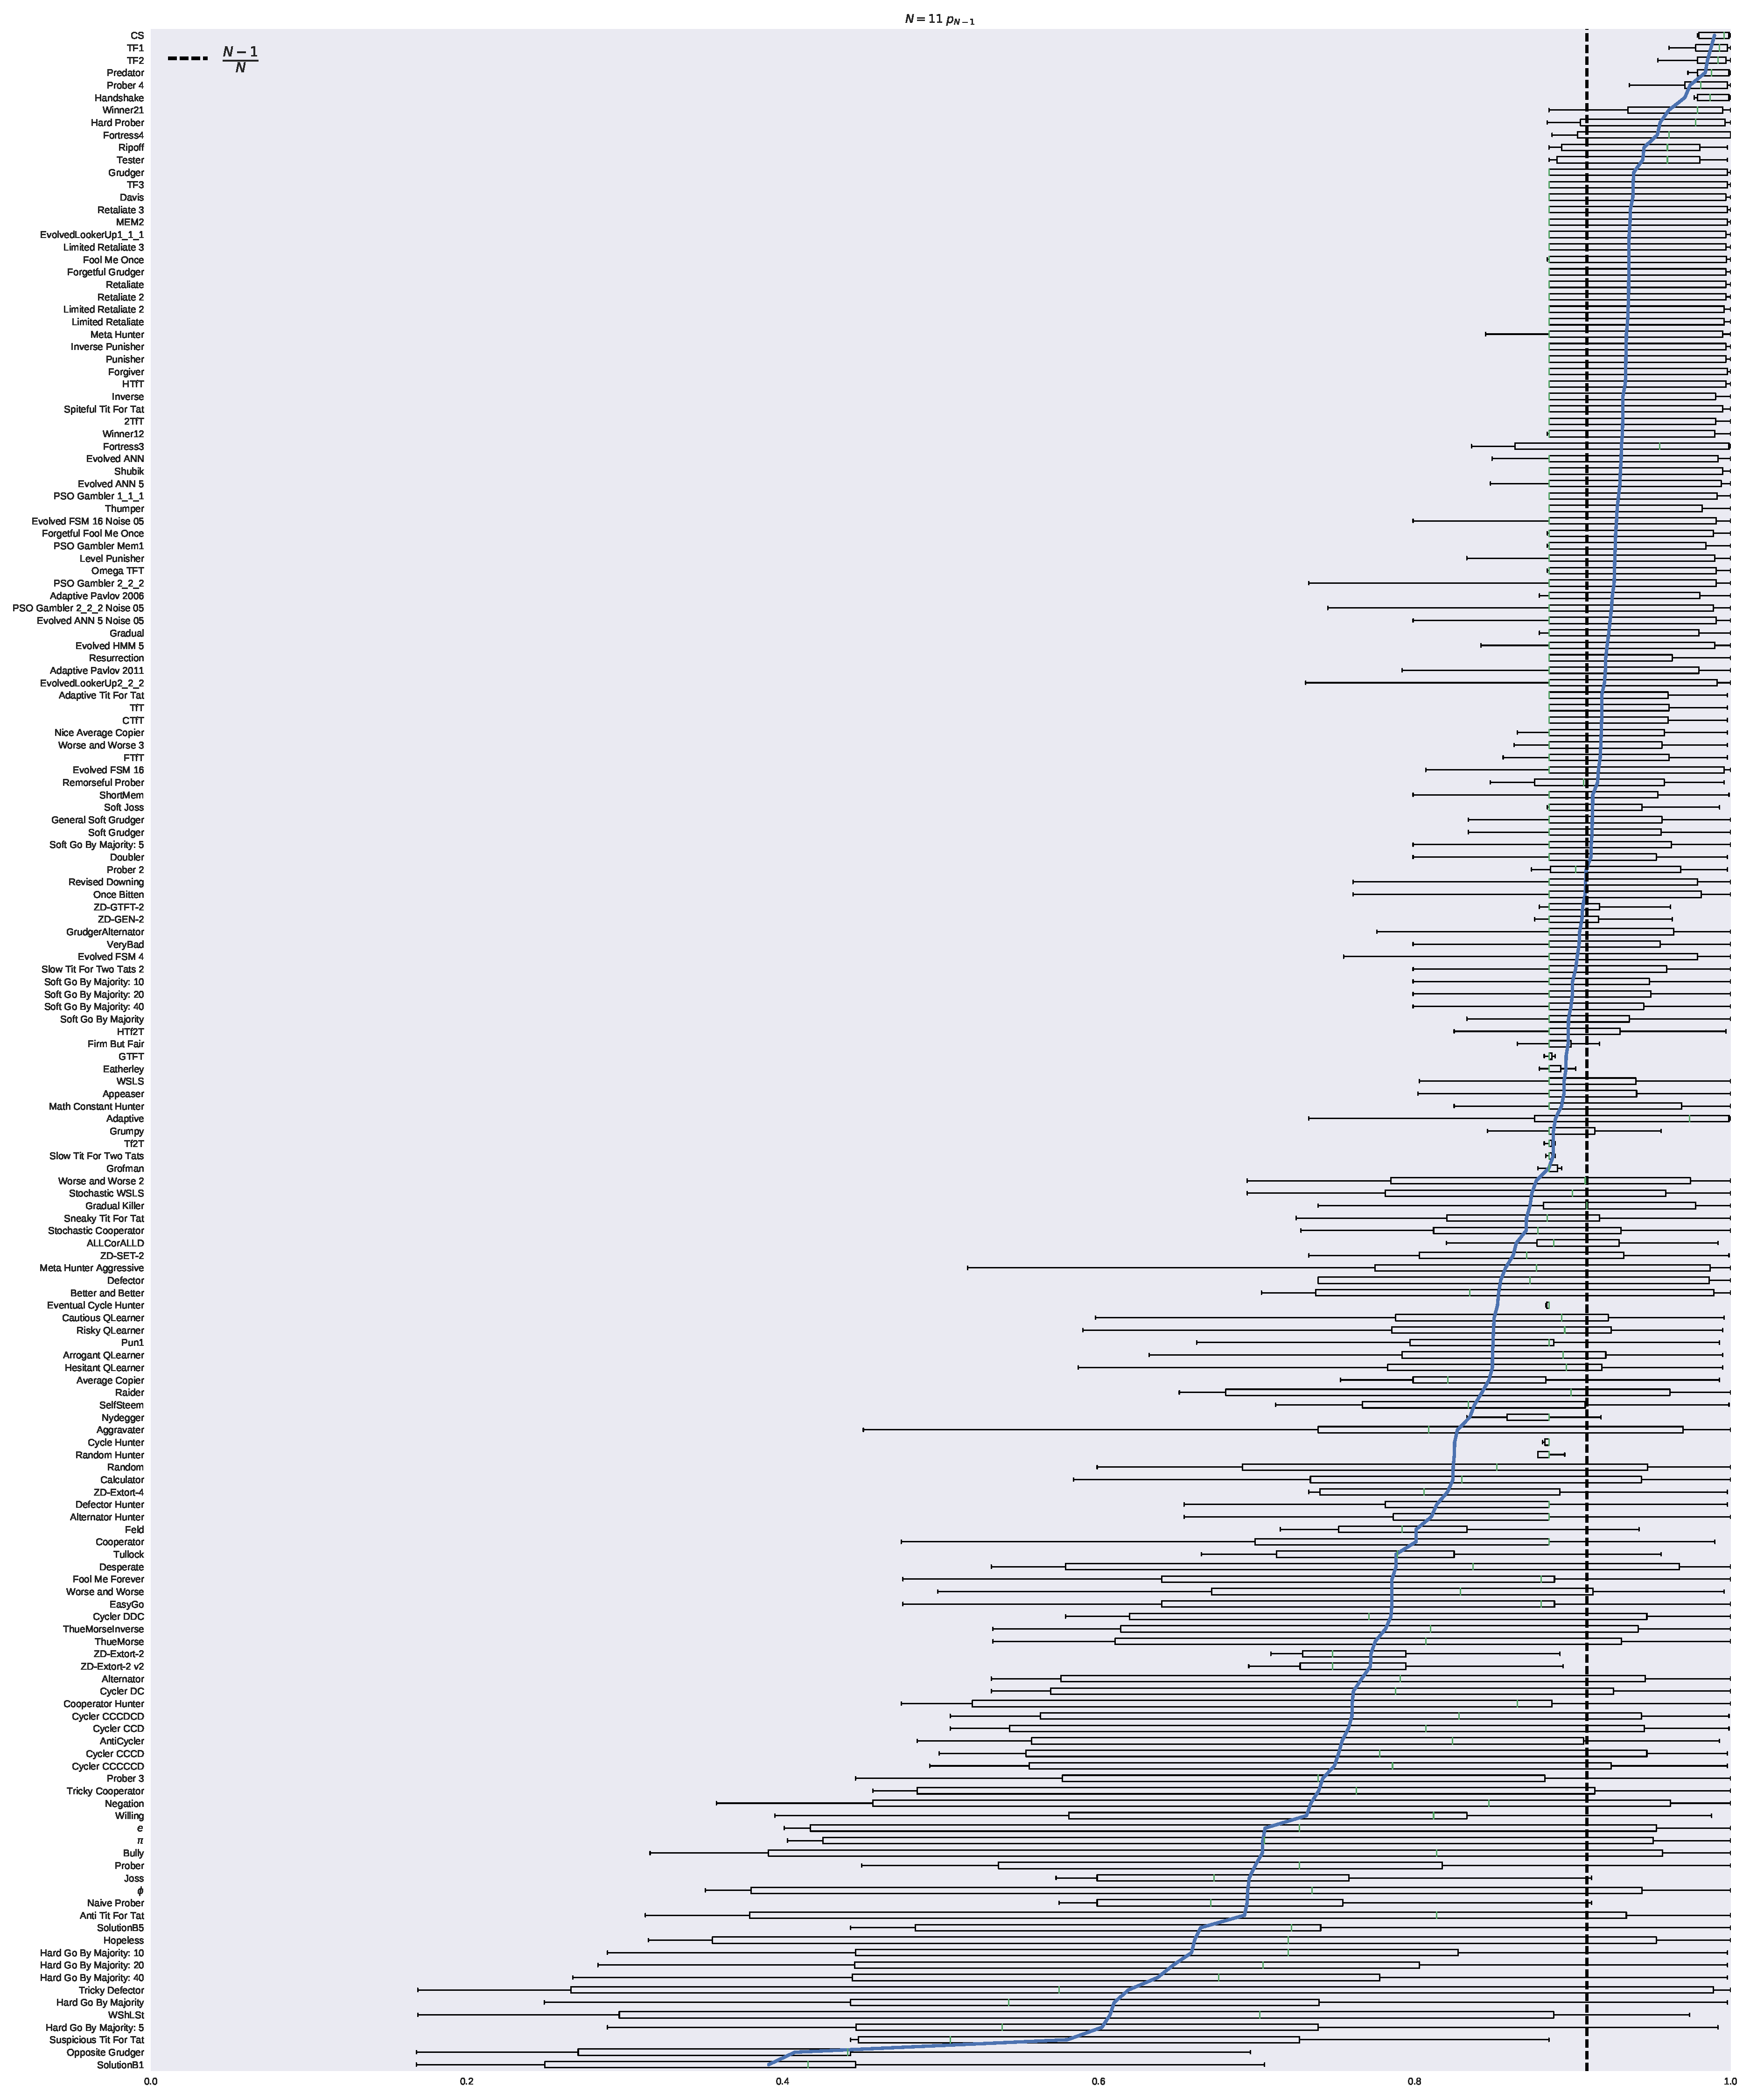
\includegraphics[width=\textwidth]{img/boxplot_11_resist.pdf}
    \caption{The fixation probabilities \(x_{N-1}\) for \(N=11\)}
\end{figure}

\begin{figure}[!hbtp]
    \centering
    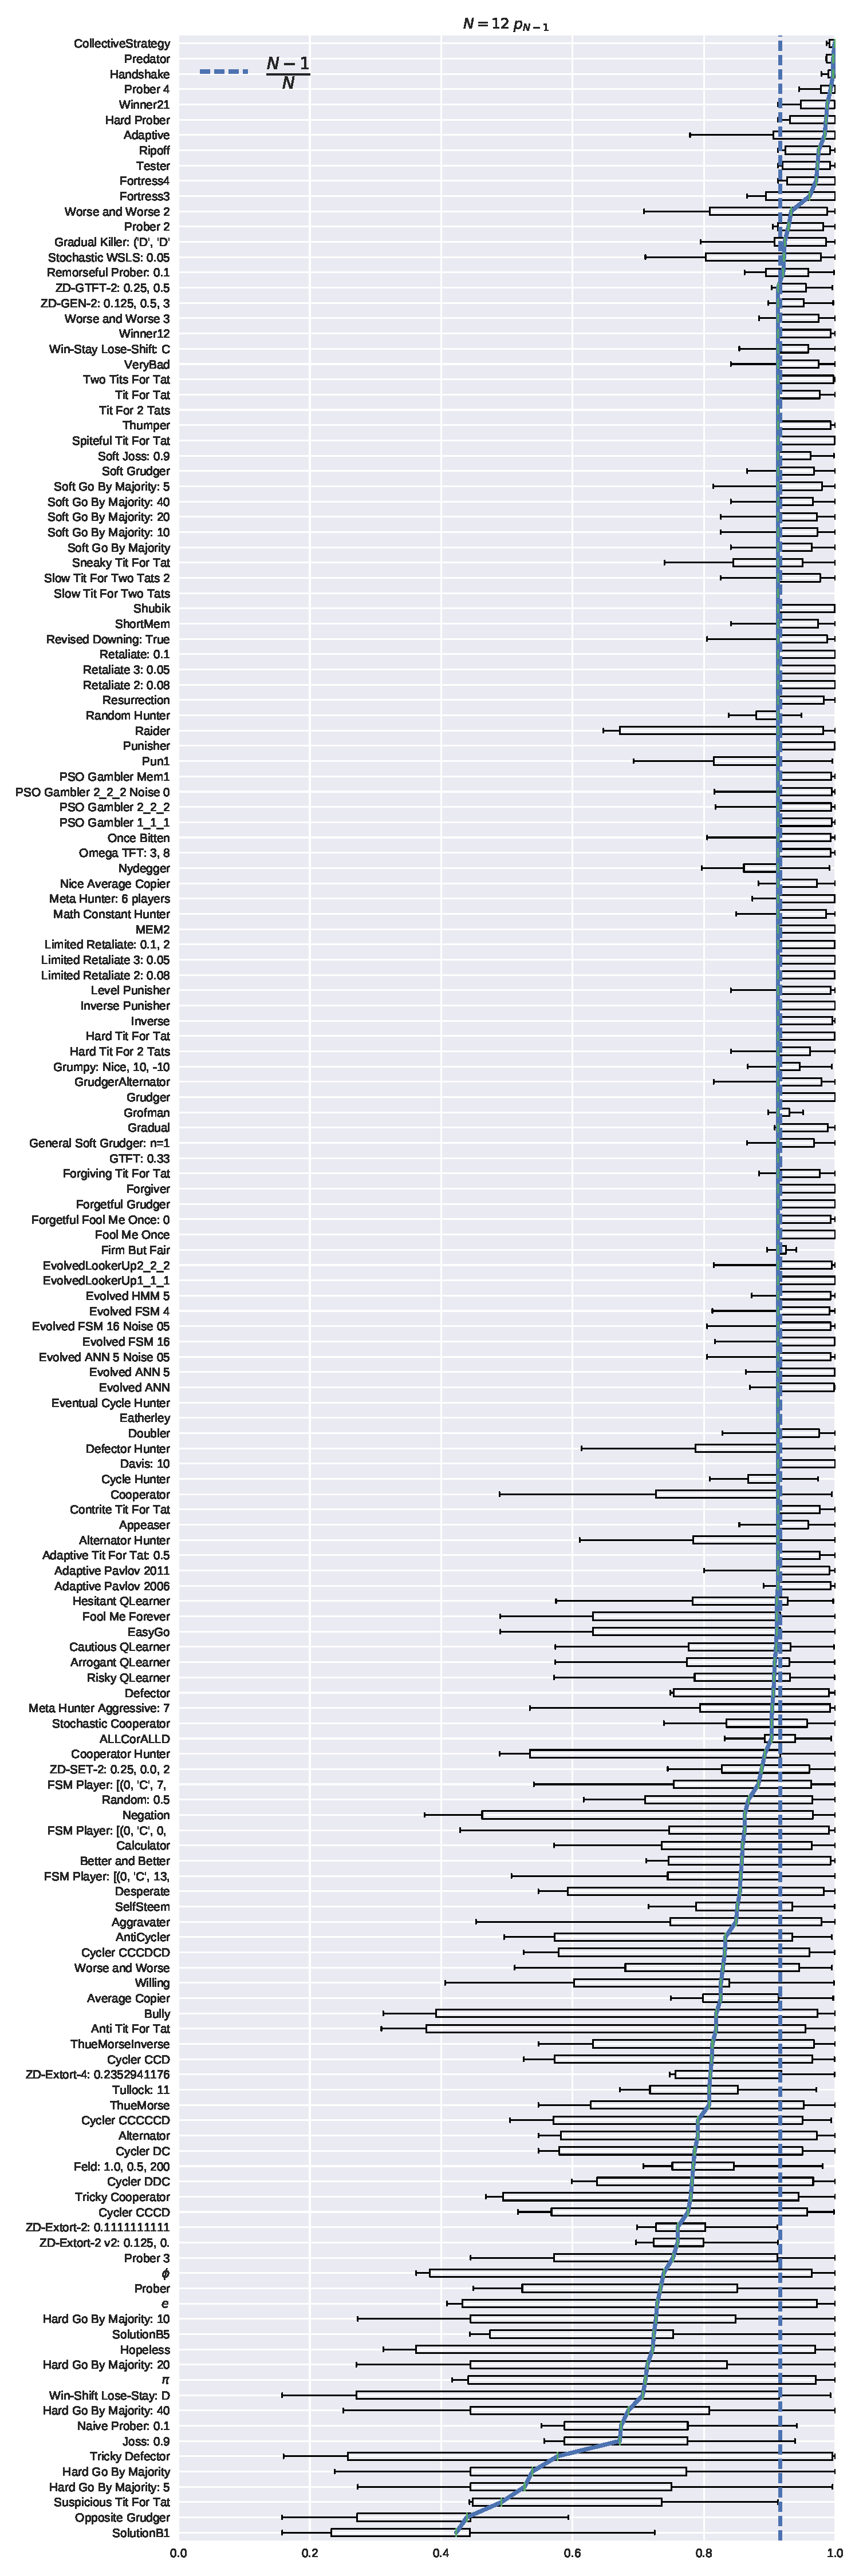
\includegraphics[width=\textwidth]{img/boxplot_12_resist.pdf}
    \caption{The fixation probabilities \(x_{N-1}\) for \(N=12\)}
\end{figure}

\begin{figure}[!hbtp]
    \centering
    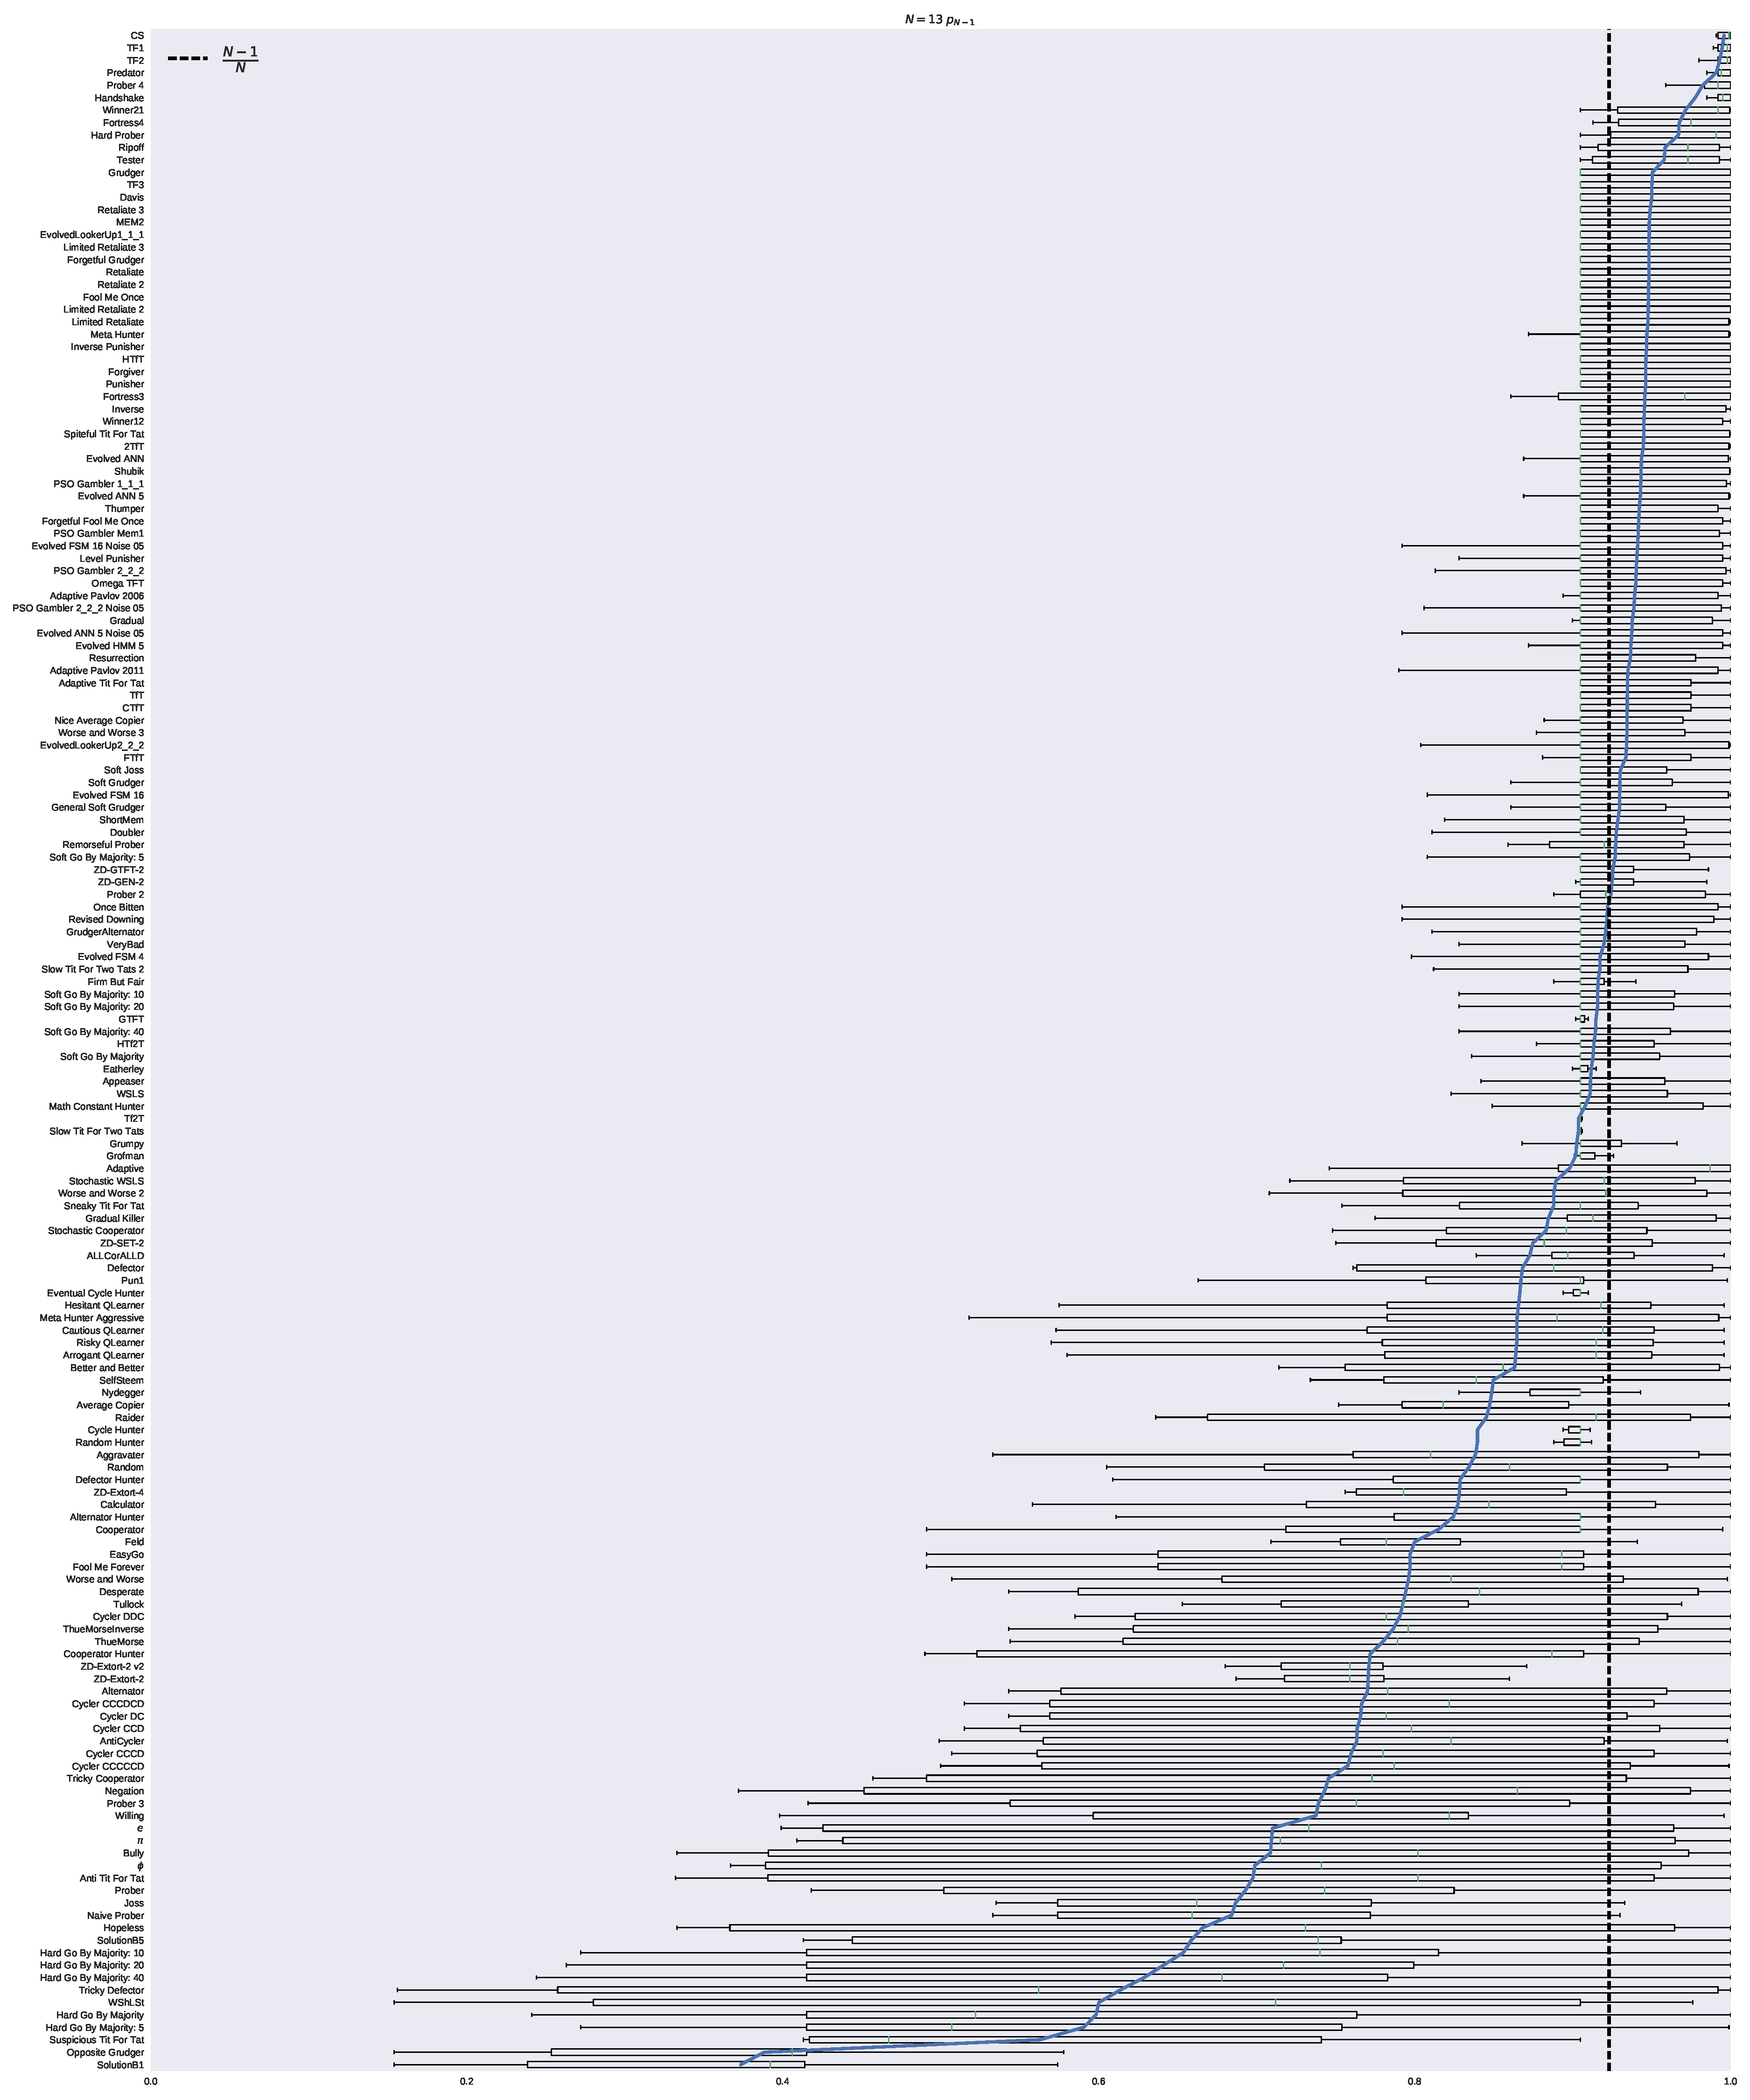
\includegraphics[width=\textwidth]{img/boxplot_13_resist.pdf}
    \caption{The fixation probabilities \(x_{N-1}\) for \(N=13\)}
\end{figure}

\begin{figure}[!hbtp]
    \centering
    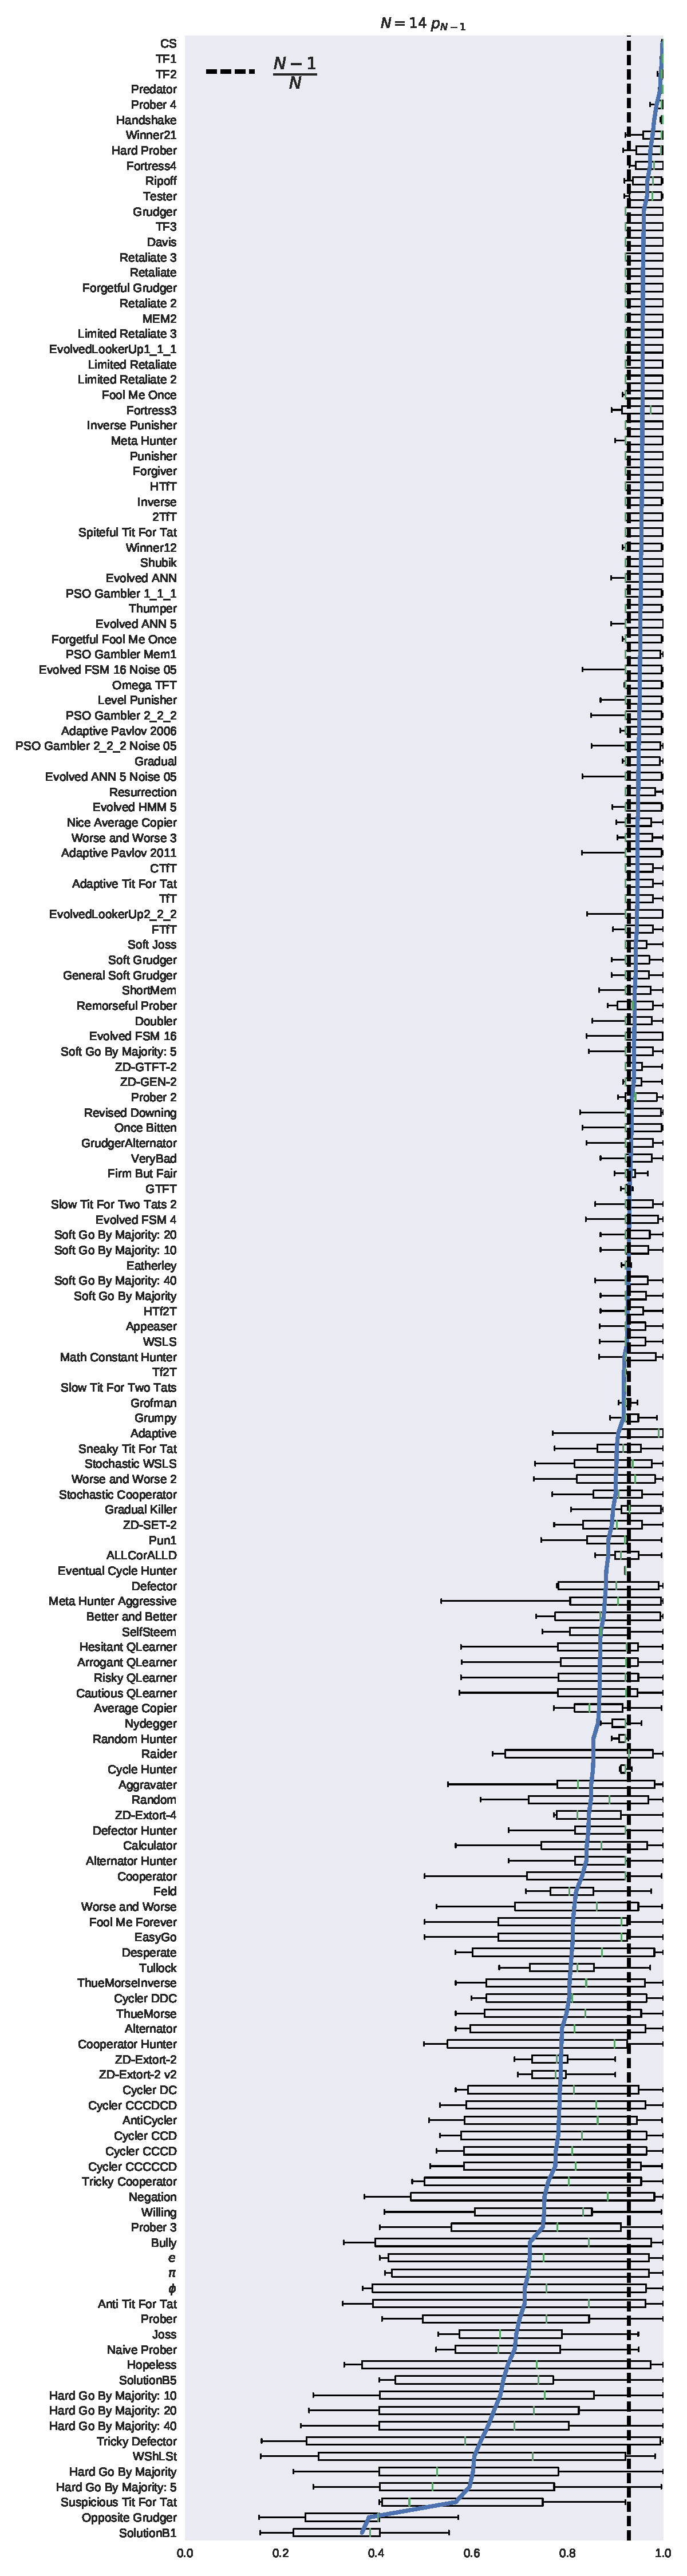
\includegraphics[width=\textwidth]{img/boxplot_14_resist.pdf}
    \caption{The fixation probabilities \(x_{N-1}\) for \(N=14\)}
    \label{resistance-14}
\end{figure}


\begin{figure}[!hbtp]
    \centering
    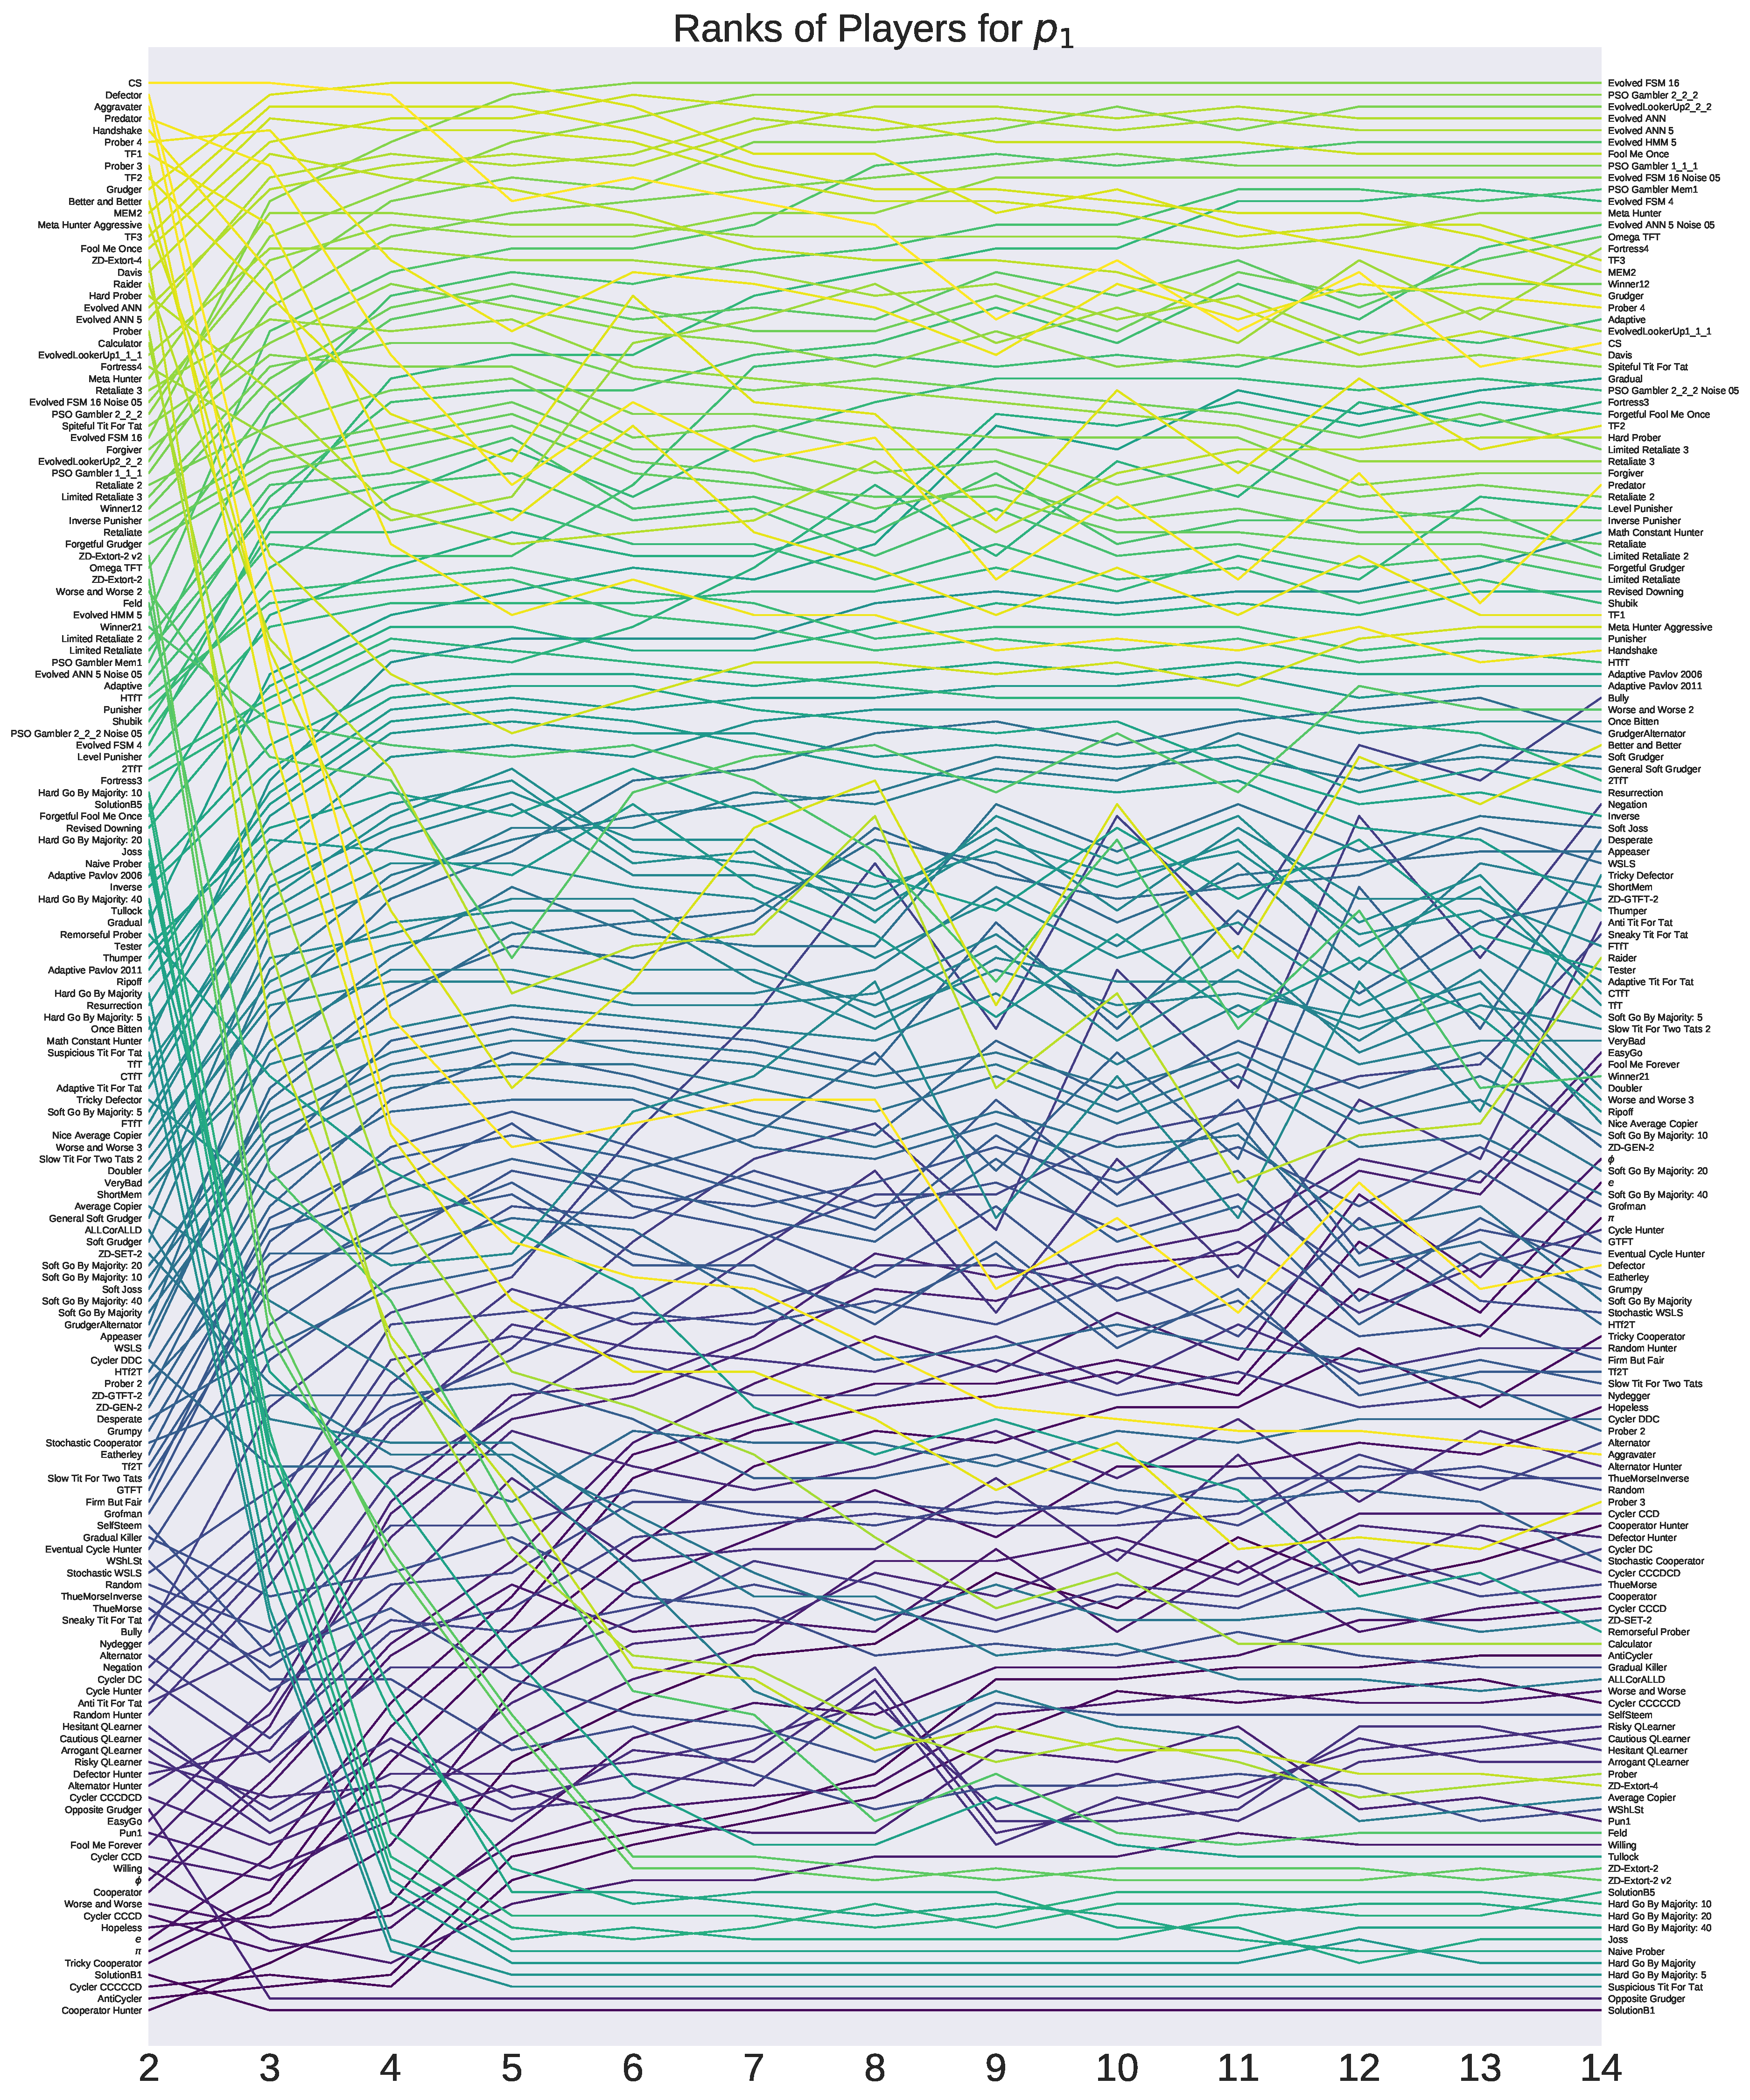
\includegraphics[width=\columnwidth]{img/average_rank_vs_population_size_invade.pdf}
    \caption{\textbf{Invasion}: Ranks of all strategies according to \(x_1\) for different population sizes.}
    \label{fig:ranks_v_size_invade}
\end{figure}

\begin{figure}[!hbtp]
    \centering
    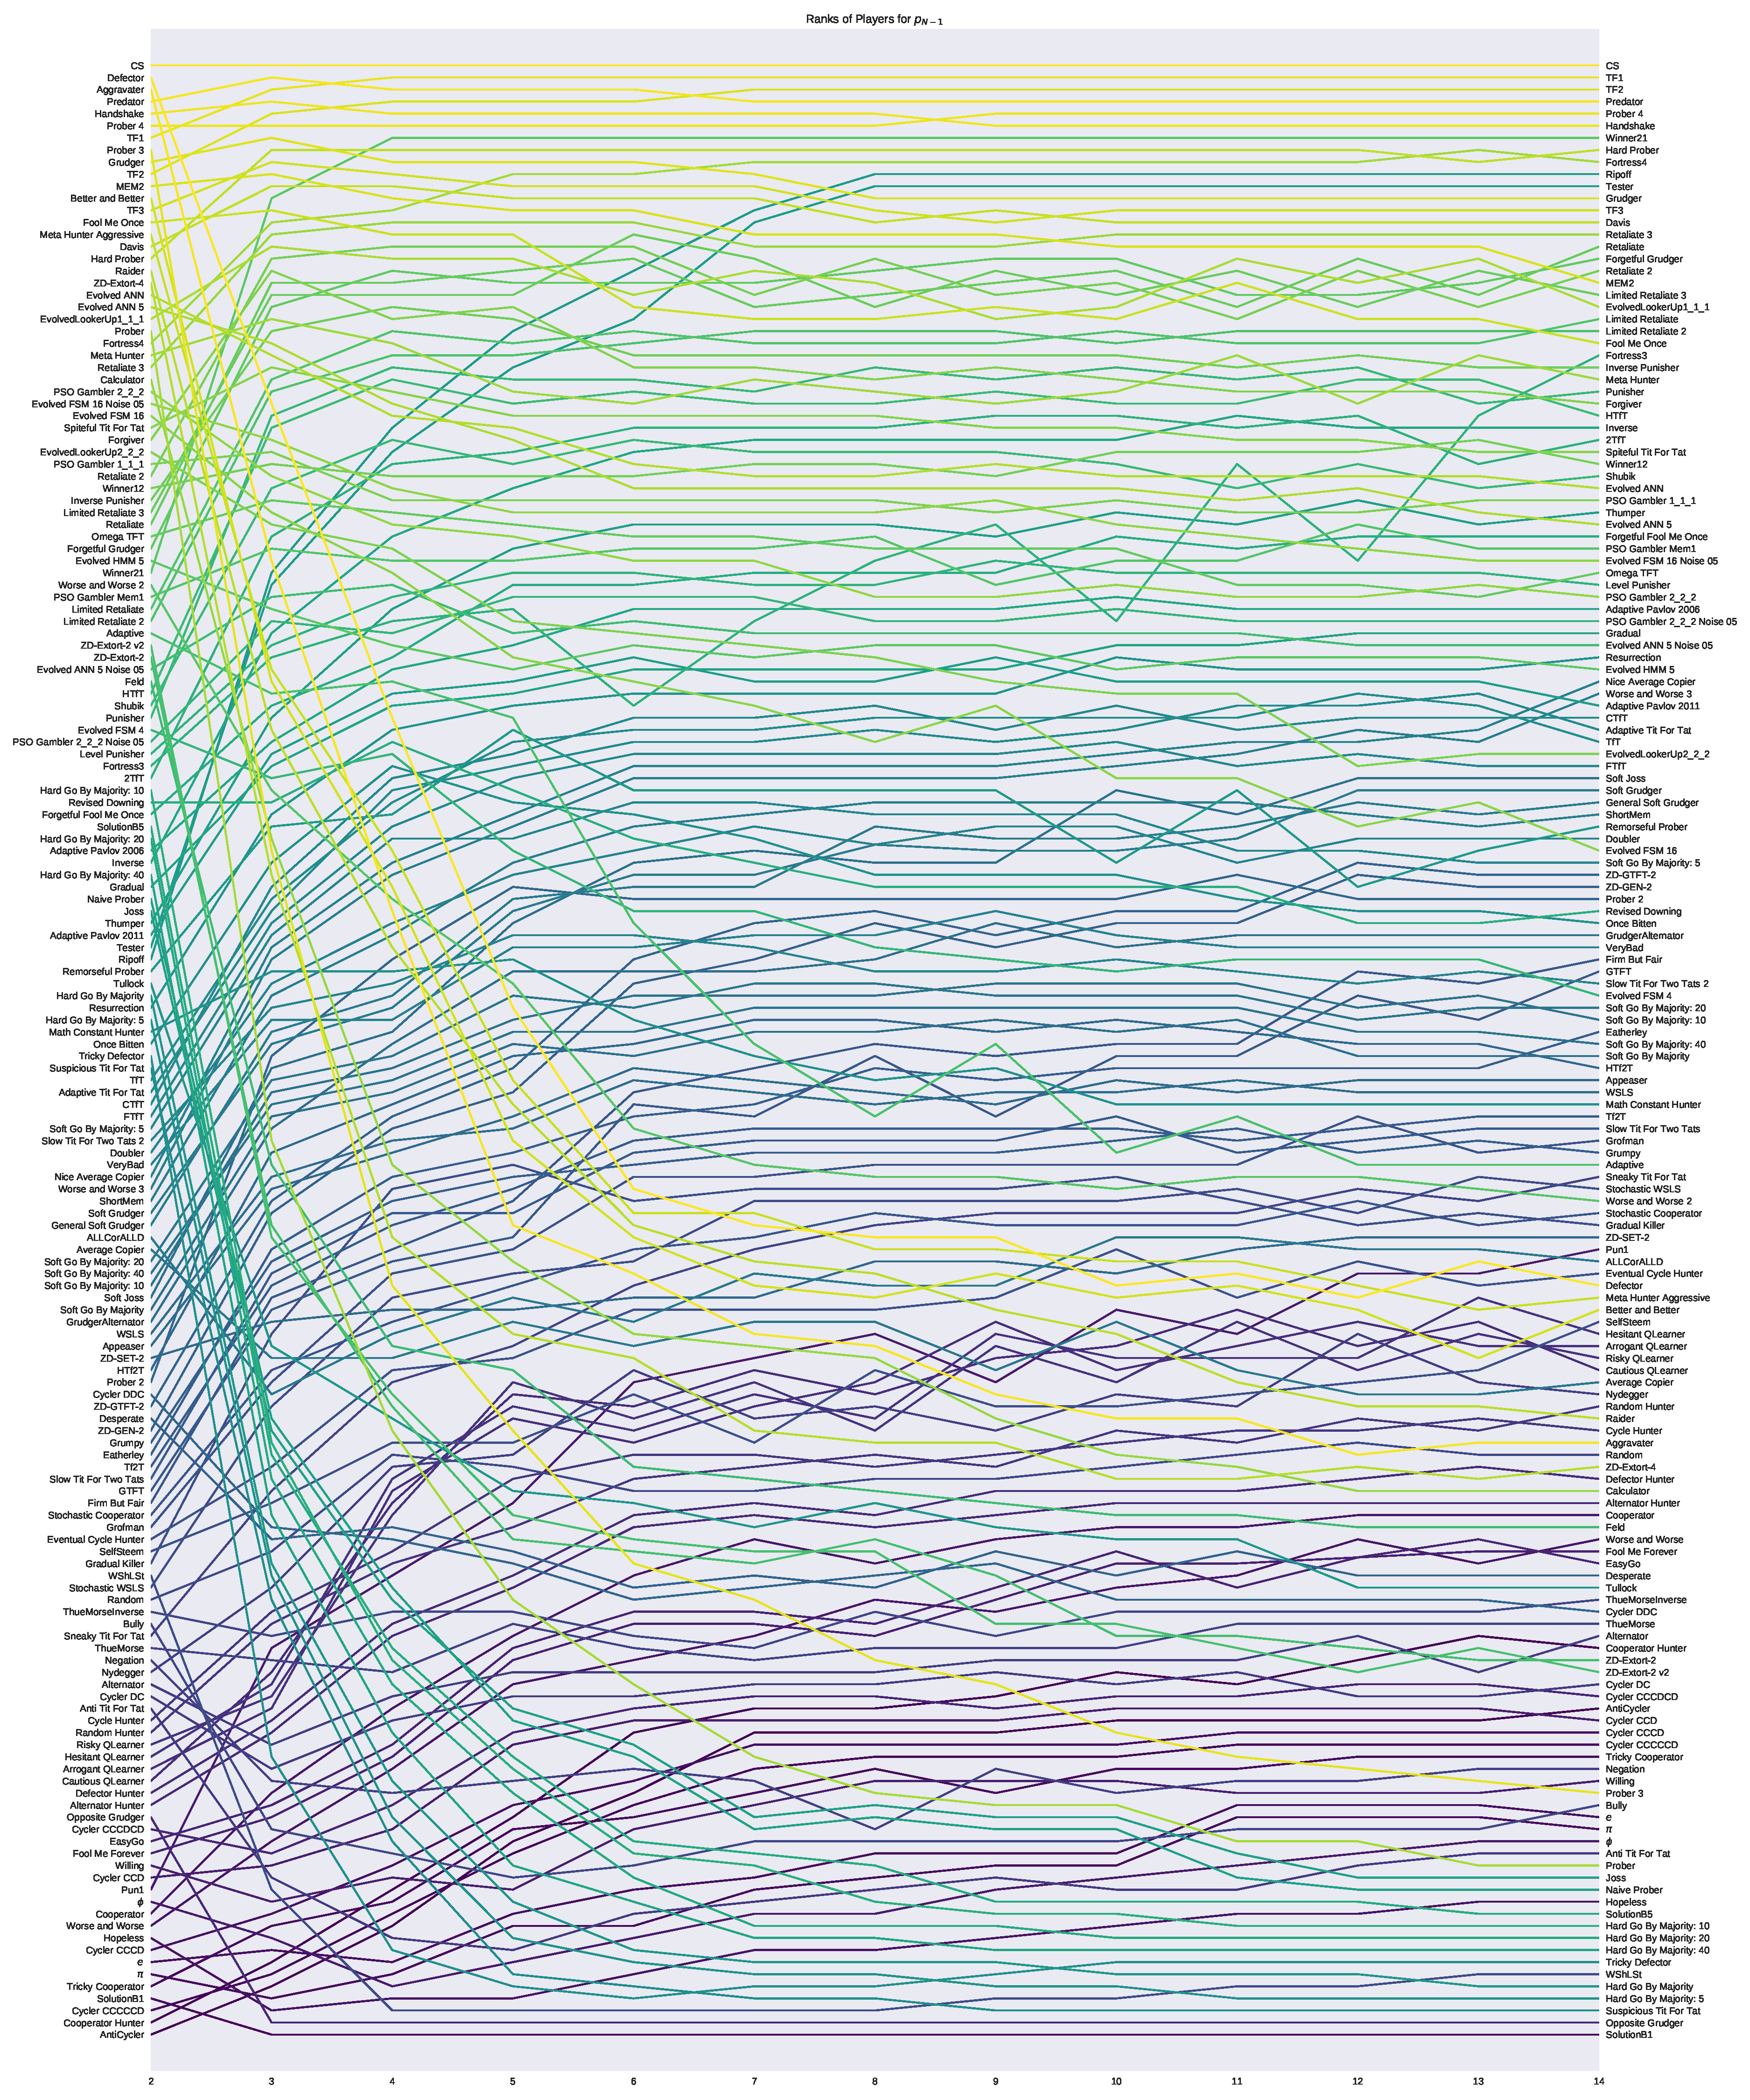
\includegraphics[width=\columnwidth]{img/average_rank_vs_population_size_resist.pdf}
    \caption{\textbf{Resistance}: Ranks of all strategies according to \(x_{N-1}\) for different
    population sizes.}
    \label{fig:ranks_v_size_resist}
\end{figure}

\begin{figure}[!hbtp]
    \centering
    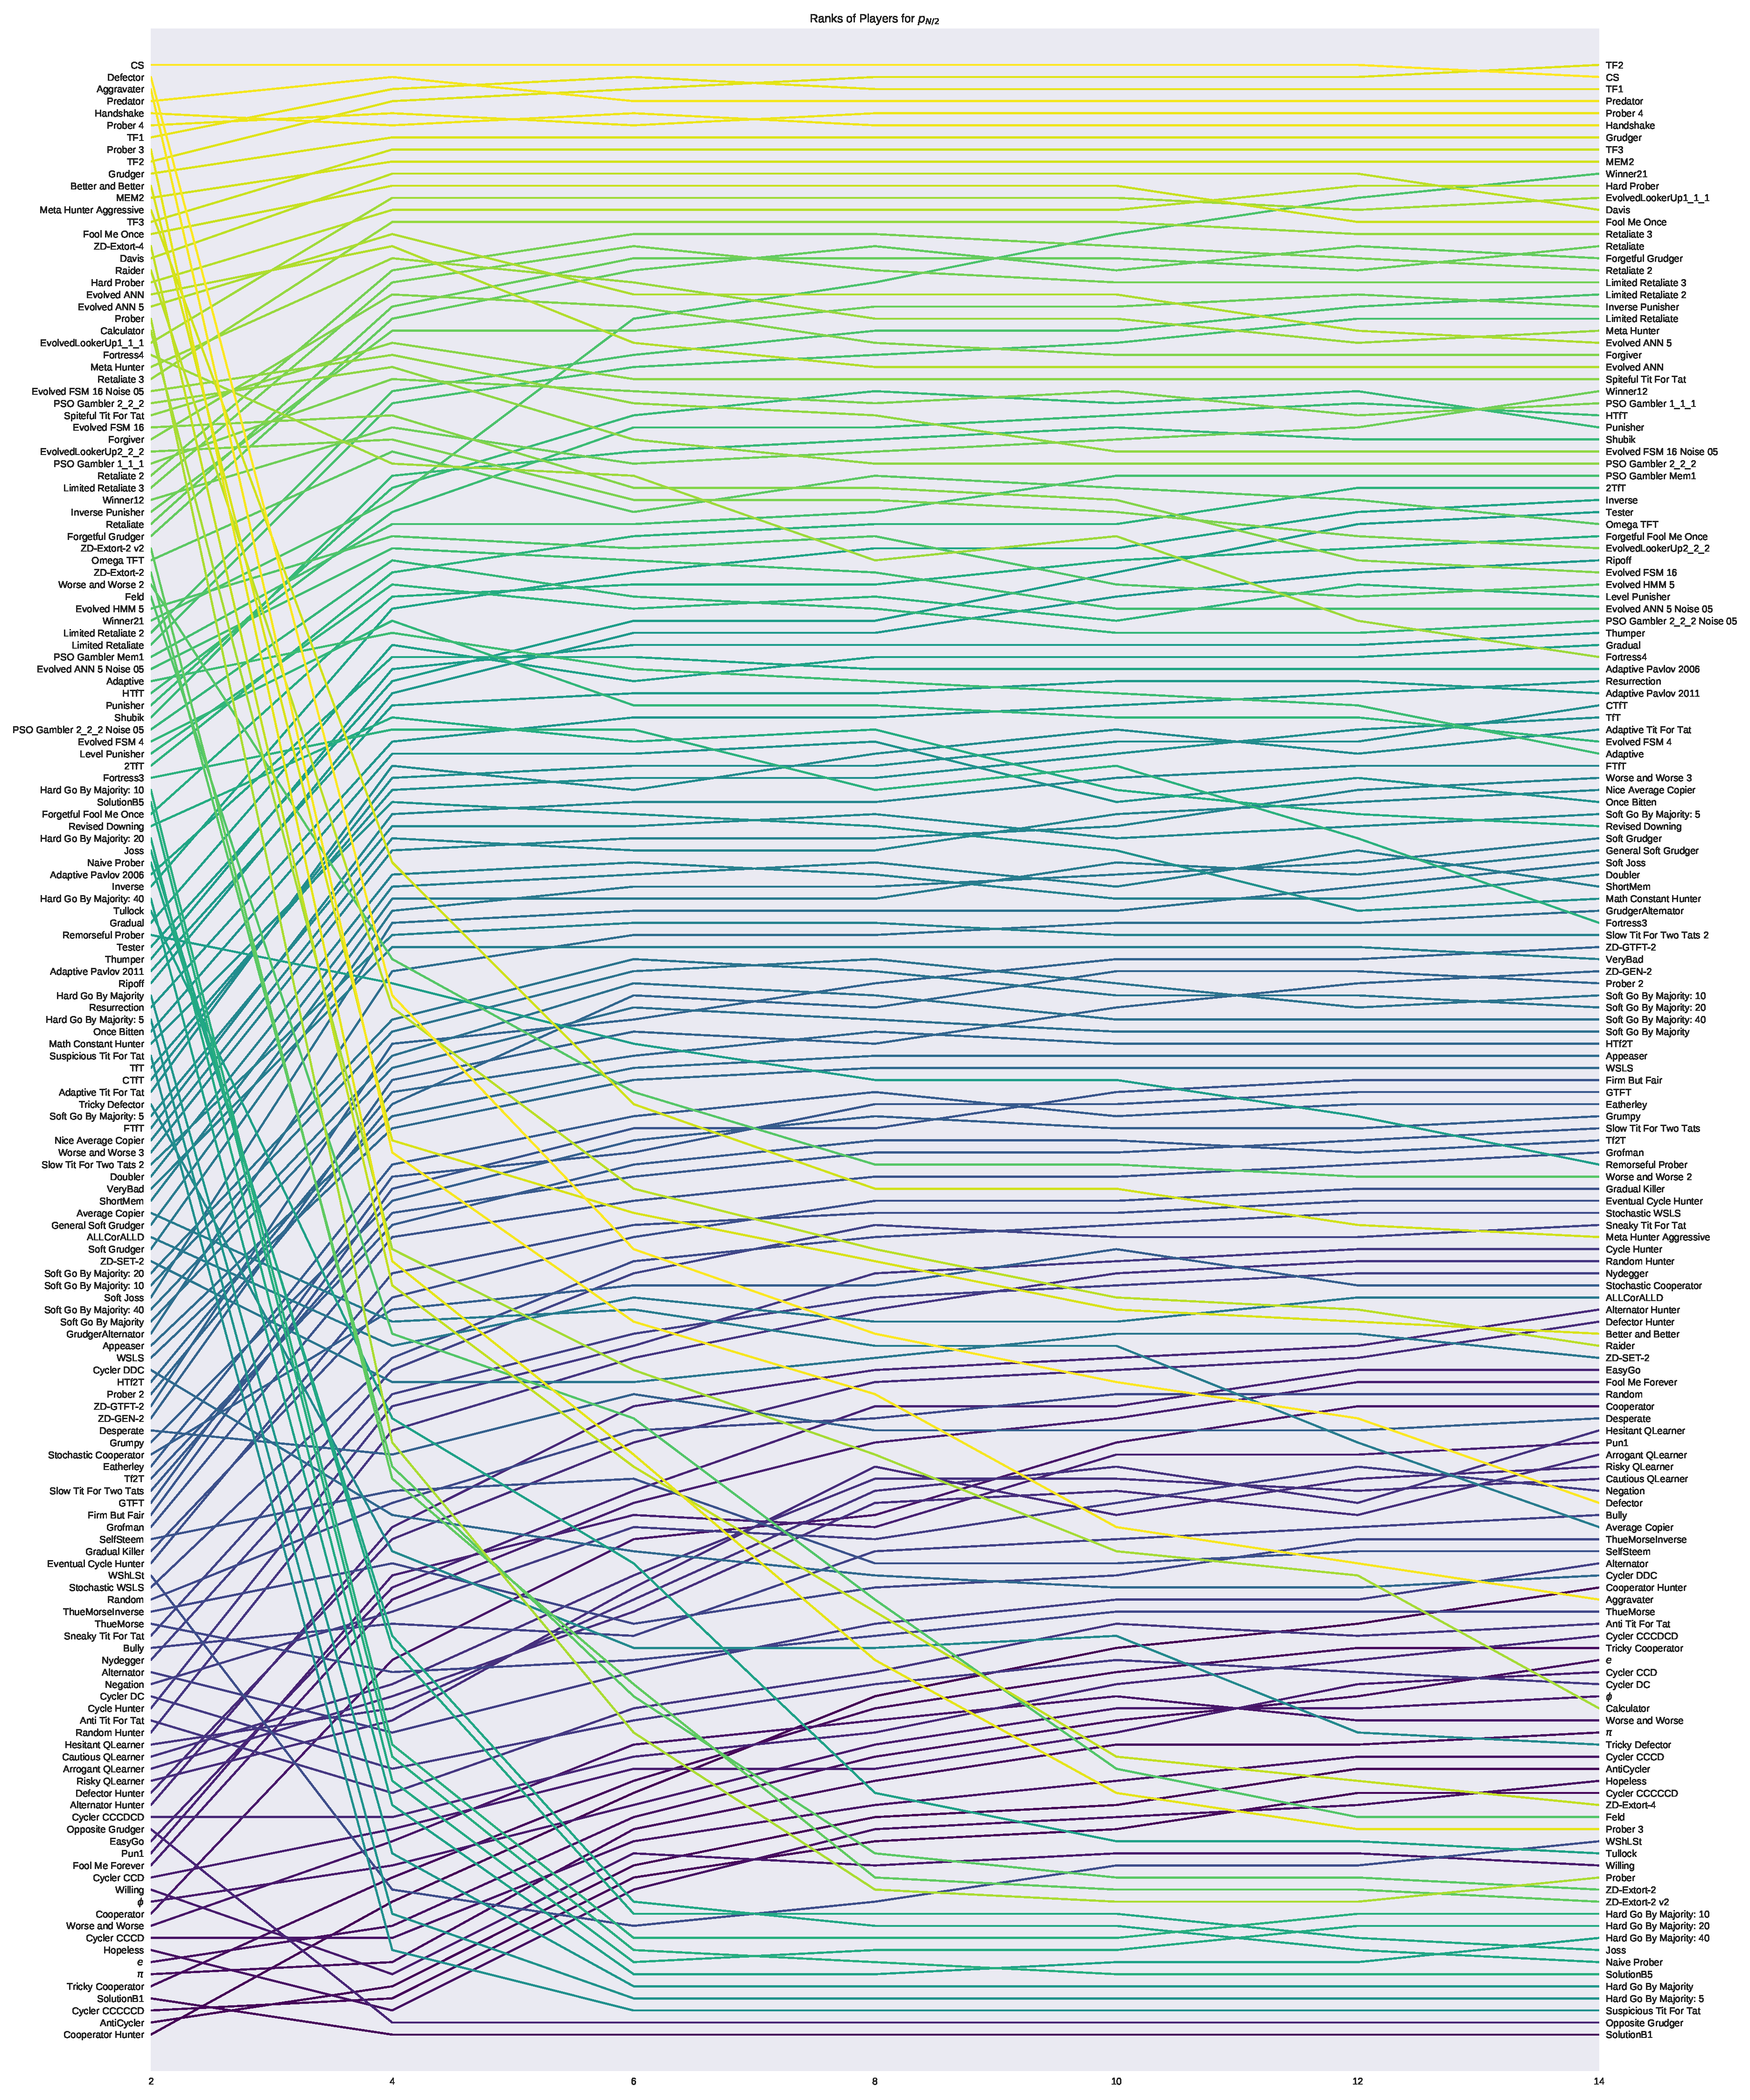
\includegraphics[width=\columnwidth]{img/average_rank_vs_population_size_coexist.pdf}
    \caption{Fixation ranks of all strategies according to \(x_{N/2}\) for different
    population sizes.}
    \label{fig:ranks_v_size_coexist}
\end{figure}

\end{document}
